\documentclass [aspectratio=169]{beamer}
\beamertemplatenavigationsymbolsempty
\usetheme{Boadilla}
\usepackage{textpos} % package for the positioning
\usepackage[]{graphicx}
\usepackage{graphicx}
\usepackage{float}
\usepackage{hyperref}
\usepackage{caption}
\usepackage{subcaption}
\usepackage{algorithm,algpseudocode}
\usepackage[export]{adjustbox}
\usepackage{tikz}
\usepackage[square,numbers]{natbib}
\usepackage[byname]{smartref}
\usetikzlibrary{positioning}
\usetikzlibrary{arrows, shapes, decorations, automata, backgrounds, fit, petri, calc}

\newcommand*{\logofont}{\fontfamily{phv}\selectfont}

\definecolor{uwopurple}{RGB}{79,38,131} % official purple color for uwo

\title[]{\vspace{60pt} \\
Status and plans} % Change the lecture topic right here!
%\subtitle{n}
\author[]{J.J. Gómez Cadenas}
\institute[]{Donostia International Physics Center}
\date{\today}

% Math notations
\newtheorem{thm}{Theorem}[section]
\newtheorem{lem}[thm]{Lemma}

\newtheorem{defn}[thm]{Definition}
\newtheorem{eg}[thm]{Example}
\newtheorem{ex}[thm]{Exercise}
\newtheorem{conj}[thm]{Conjecture}
\newtheorem{cor}[thm]{Corollary}
\newtheorem{claim}[thm]{Claim}
\newtheorem{rmk}[thm]{Remark}

\newcommand{\ie}{\emph{i.e.} }
\newcommand{\cf}{\emph{cf.} }
\newcommand{\into}{\hookrightarrow}
\newcommand{\dirac}{\slashed{\partial}}
\newcommand{\bbonu}{\ensuremath{\beta\beta0\nu}}
\newcommand{\bbtnu}{\ensuremath{\beta\beta2\nu}}
\newcommand{\mbb}{\ensuremath{m_{\beta\beta}}}
\newcommand{\qbb}{\ensuremath{Q_{\beta\beta}}}
\newcommand{\mbbsq}{\ensuremath{m_{\beta\beta}^2}}
\newcommand{\tonu}{\ensuremath{(T_{1/2}^{0\nu})^{-1}}}
\newcommand{\gonu}{\ensuremath{G^{0\nu}}}
\newcommand{\monu}{\ensuremath{| M^{0\nu}|^2}}
\newcommand{\XE}{\ensuremath{{}^{136}{\rm Xe}}}
\newcommand{\GE}{\ensuremath{{}^{76}{\rm Ge}}}
\newcommand{\TE}{\ensuremath{{}^{130}{\rm Te}}}
\newcommand{\TL}{\ensuremath{{}^{208}{\rm Tl}}}
\newcommand{\BI}{\ensuremath{{}^{214}{\rm Bi}}}
\newcommand{\XES}{\ensuremath{{}^{137}{\rm Xe}}}
\newcommand{\MO}{\ensuremath{{}^{100}{\rm Mo}}}
%\newcommand{\bbtnu}{\ensuremath{\beta\beta 2\nu}}
%\newcommand{\bbonu}{\ensuremath{\beta\beta 0\nu}}
\newcommand{\KR}{\ensuremath{{}^{83}{\rm Kr}}}
\newcommand{\nne}{\ensuremath{\bar{N}_e}}
\newcommand{\nng}{\ensuremath{\bar{N}_\gamma}}
\newcommand{\so}{\ensuremath{\rm S_1}}
\newcommand{\st}{\ensuremath{\rm S_2}}
\newcommand{\tz}{\ensuremath{\rm t_0}}
\newcommand{\R}{\mathbb{R}}
\newcommand{\C}{\mathbb{C}}
\newcommand{\Z}{\mathbb{Z}}
\newcommand{\N}{\mathbb{N}}
\newcommand{\Q}{\mathbb{Q}}
\newcommand{\LieT}{\mathfrak{t}}
\newcommand{\T}{\mathbb{T}}
\newcommand{\A}{\mathds{A}}
\newcommand{\E}{\mathbb{E}}
\newcommand{\Prob}{\mathbb{P}}
\newcommand{\Var}{\text{Var}}
\newcommand\equalhat{%
\let\savearraystretch\arraystretch
\renewcommand\arraystretch{0.3}
\begin{array}{c}
\stretchto{
    \scalerel*[\widthof{=}]{\wedge}
    {\rule{1ex}{3ex}}%
}{0.5ex}\\ 
=%
\end{array}
\let\arraystretch\savearraystretch
}

% set color
\setbeamercolor{title in head/foot}{bg=white}
\setbeamercolor{author in head/foot}{bg=white}
\setbeamercolor{date in head/foot}{fg=uwopurple}
\setbeamercolor{date in head/foot}{bg=white}
\setbeamercolor{title}{fg=uwopurple}
\setbeamerfont{title}{series=\bfseries}
\setbeamercolor{frametitle}{fg=uwopurple}
\setbeamerfont{frametitle}{series=\bfseries}
\setbeamercolor{block title}{bg=uwopurple!30,fg=black}
\setbeamercolor{item}{fg=uwopurple}
\setbeamercolor{caption name}{fg=uwopurple!70!}


% set logo at non-title pages
%\logo{
\includegraphics[height=0.9cm]{dipc.png}\vspace*{-.45\paperheight}\hspace*{.50\paperwidth}}

\begin{document}

{
\setbeamertemplate{logo}{}
\begin{frame}
    \titlepage
    \begin{textblock*}{4cm}(0.5cm,-7.3cm)
        
\includegraphics[width=4cm]{dipc.png}
    \end{textblock*}
    \begin{textblock*}{8cm}(5.0cm,-7.0cm)
        \huge \color{uwopurple}{$\Bigr\rvert$ \hspace{0.15cm} \textbf{The NEXT experiment}} % Change the lecture # right here! 
    \end{textblock*}
\end{frame}
}

\begin{frame}{Majorana Neutrinos in one slide}
%\begin{columns}
%\column{0.40\textwidth}
 \begin{textblock*}{4cm}(1.7cm,-2.7cm)
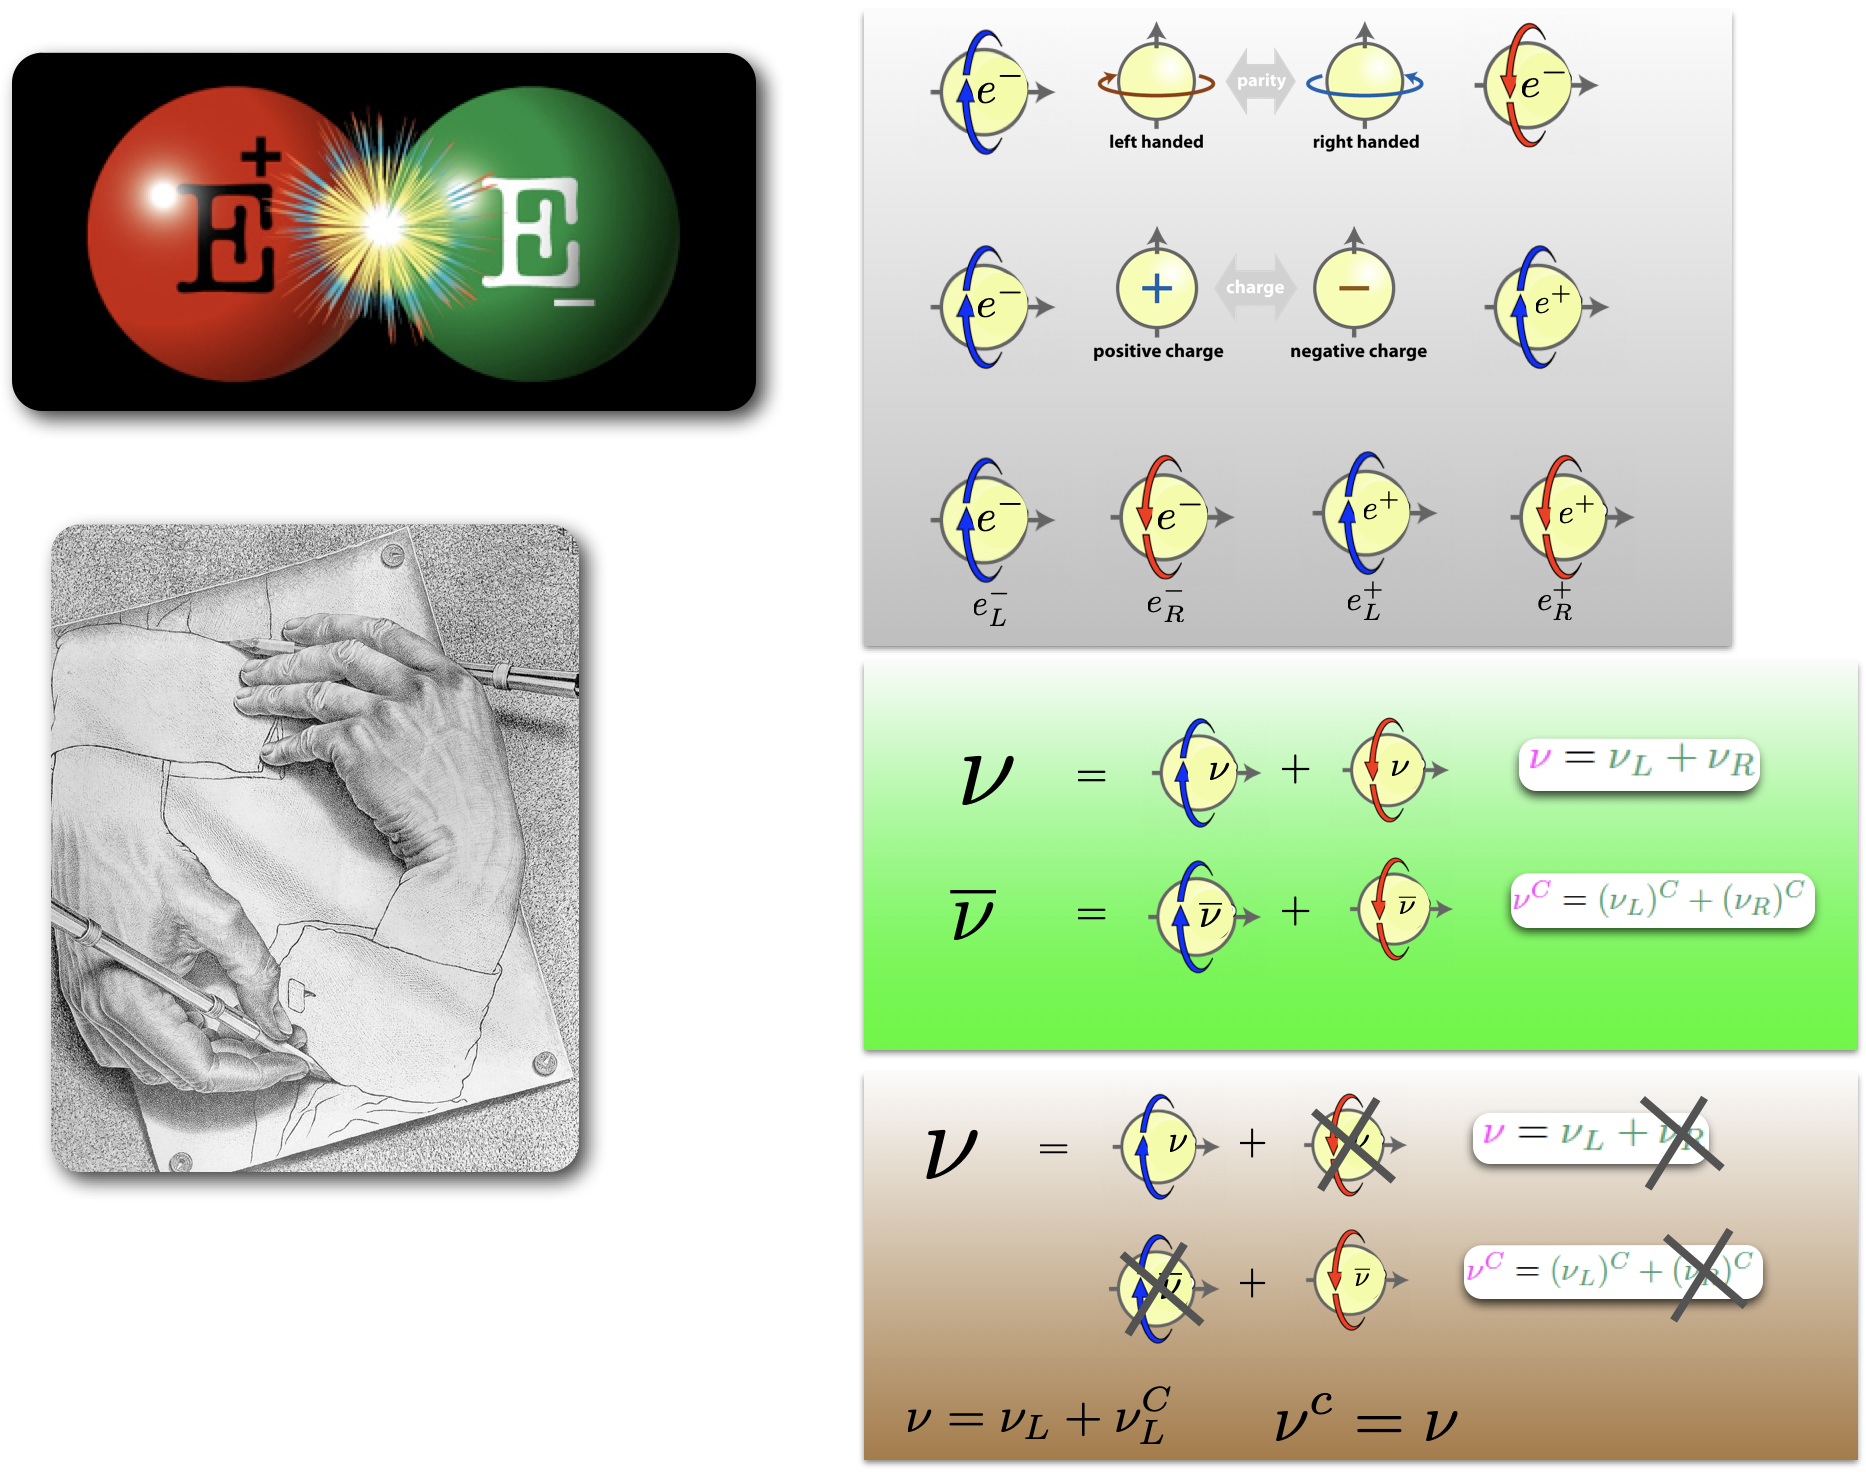
\includegraphics[scale=0.30]{majorananu.png}
 \end{textblock*}

% \column{0.5\textwidth}
%The neutrino is made, like in the Escher’s tableau of black and white chevaliers.   
%\end{columns}
\end{frame}

%%%

\begin{frame}{Majorana neutrinos \& a recipe for the Universe}
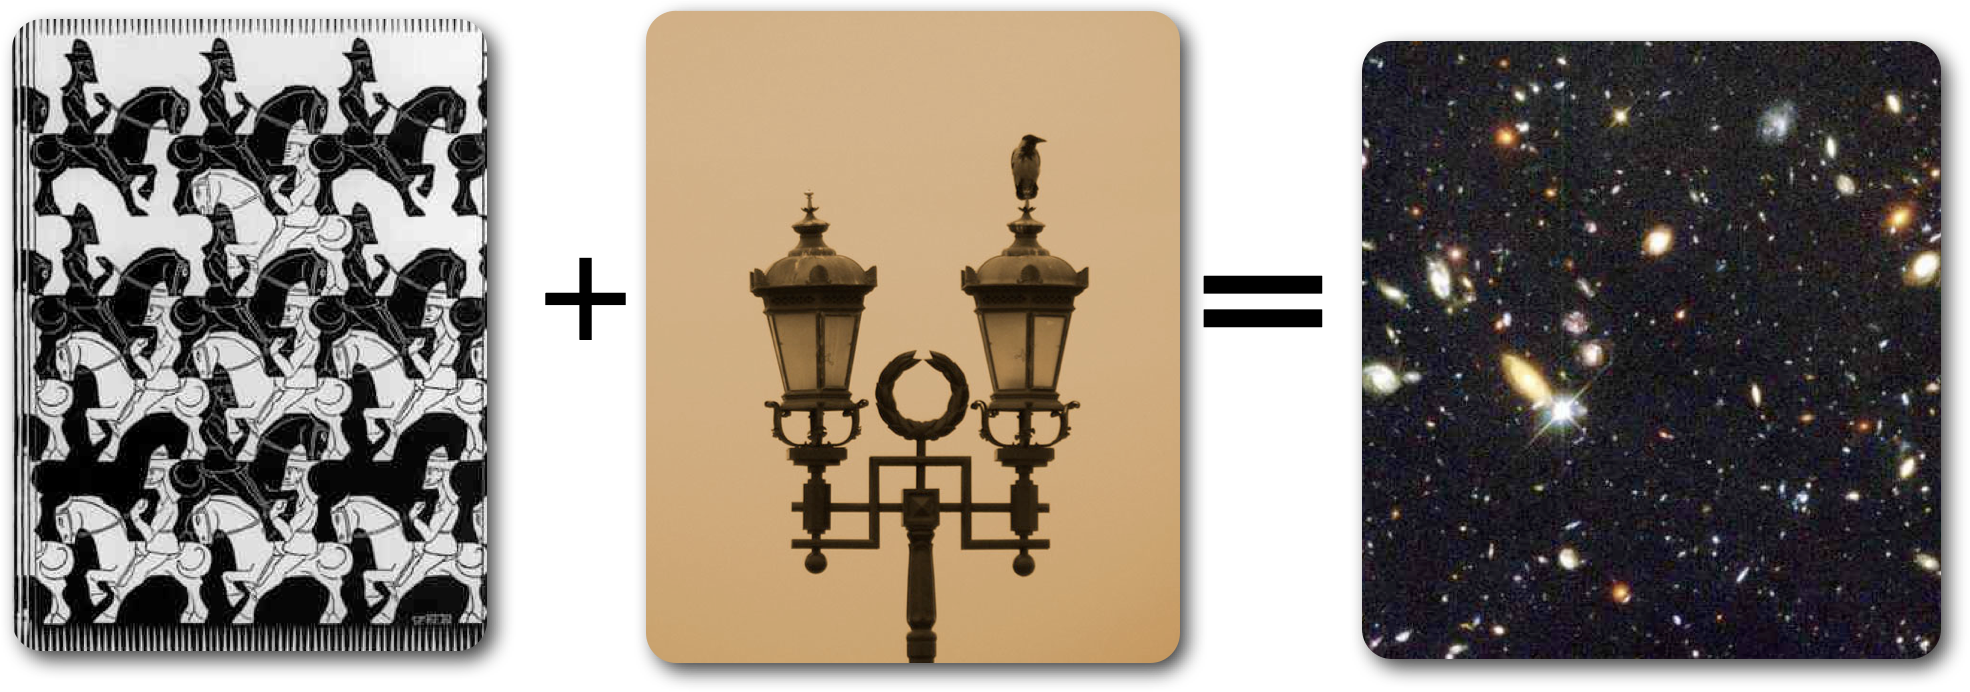
\includegraphics[scale=0.40]{Universe.png}
\end{frame}

%%



\begin{frame}{Are neutrinos Majorana Particles?}

\begin{columns}
\column{0.50\textwidth}

\includegraphics[scale=0.35]{DoubleOrNothing.png}

 \column{0.50\textwidth}
To find out play this game!   
\end{columns}
\end{frame}

%%%

\begin{frame}{$\beta\beta$. An oddity of Nature}

\begin{columns}

%

\column{0.5\textwidth}
$\bullet~$   $\beta\beta2\nu$. A rare nuclear transition $Z \rightarrow Z + 2$. Can occur only if the initial nucleus is less bound than the final nucleus, and both more than the intermediate one.

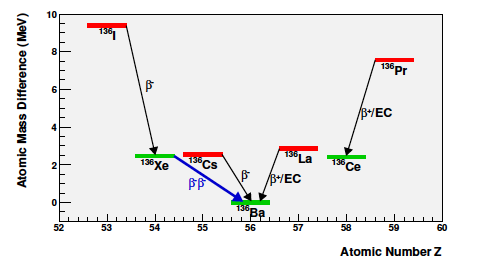
\includegraphics[scale=0.40]{xebb2nu.png}
%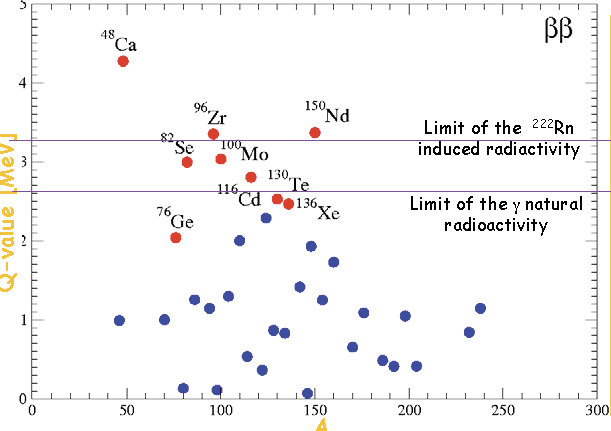
\includegraphics[scale=0.30]{betabetaisotopes.png}


 \column{0.50\textwidth}
$\bullet~$   $\beta\beta0\nu$. If and only if neutrinos are Majorana Particles

 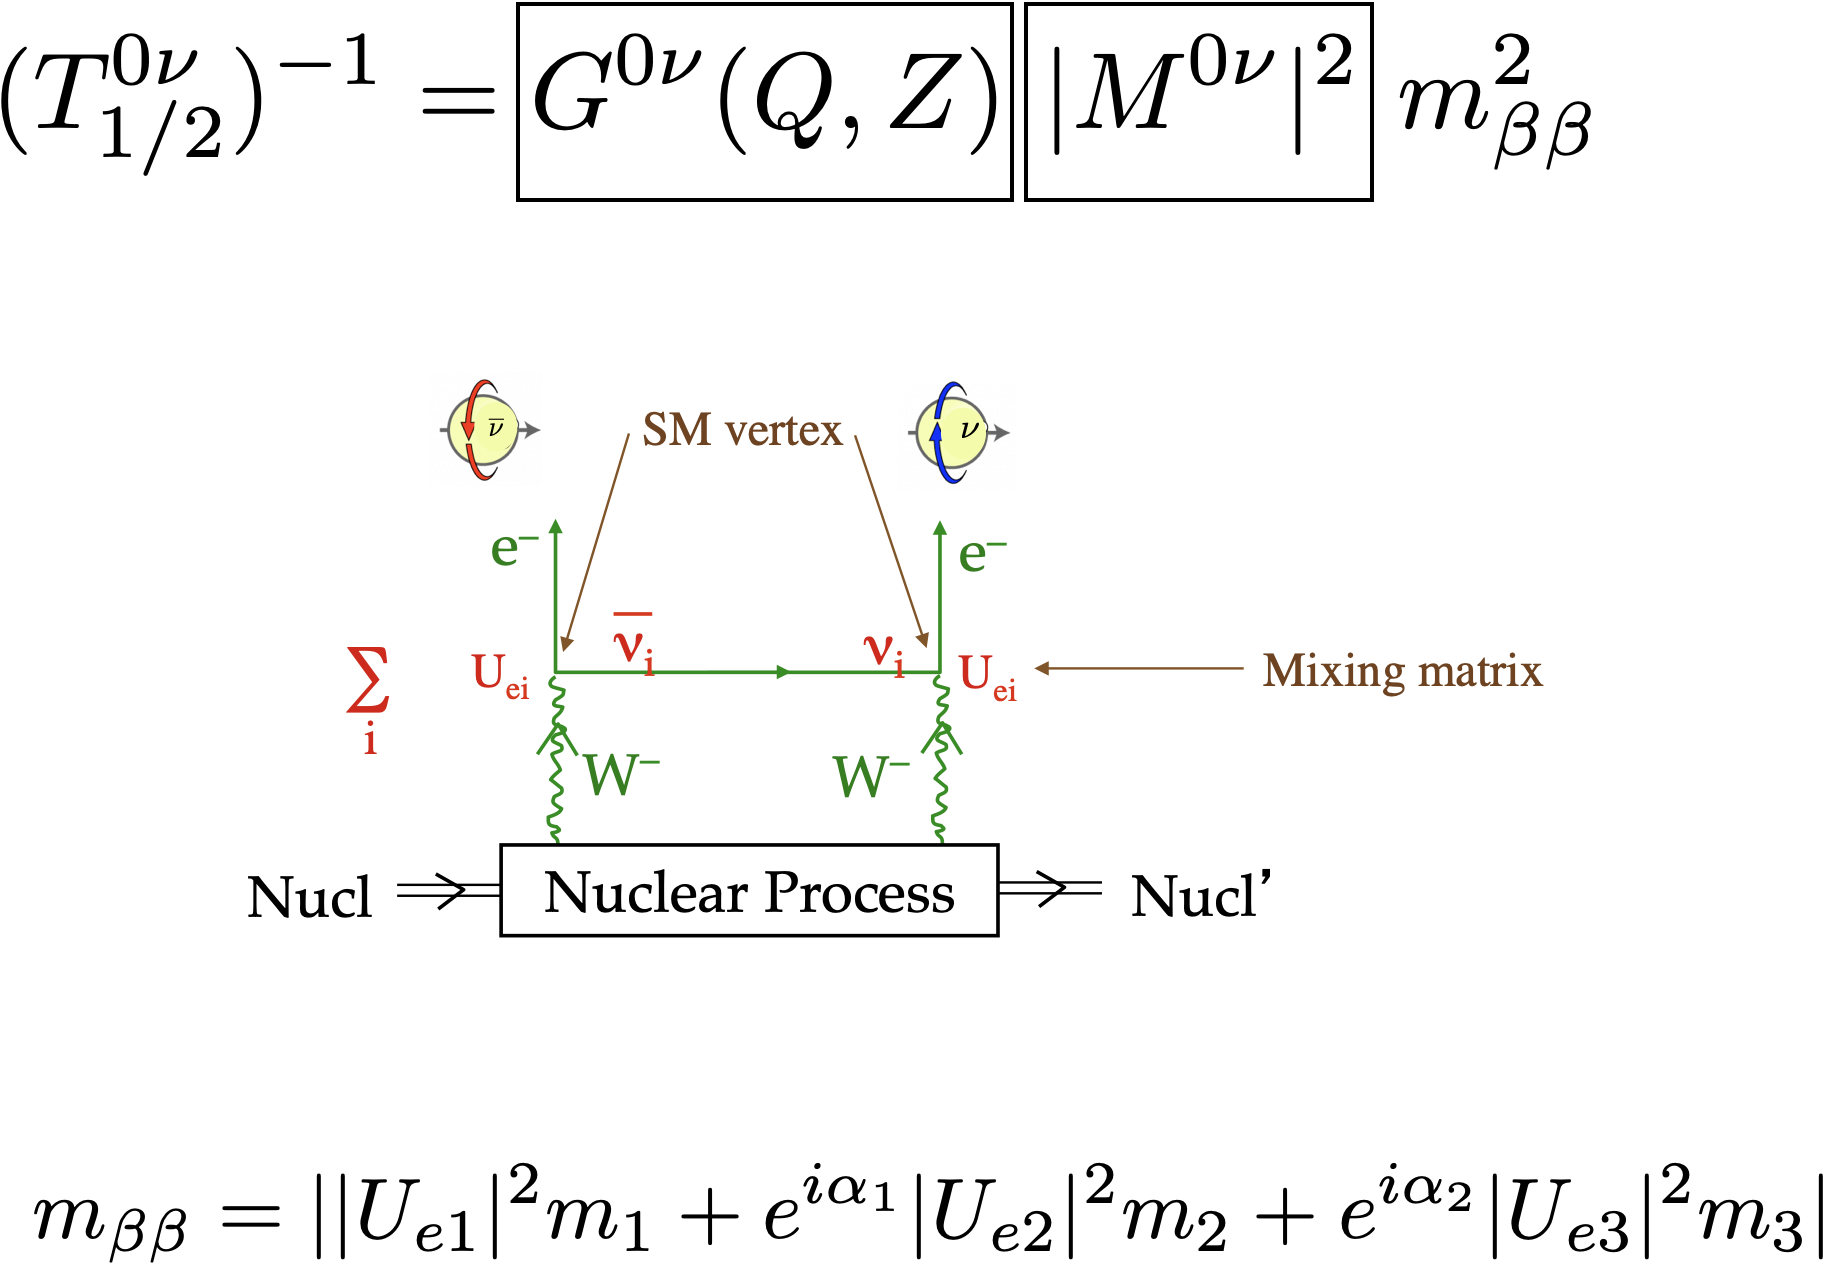
\includegraphics[scale=0.22]{bb0nu.png}
%$\bullet~$ Double beta decay is a rare nuclear transition in which a nucleus with Z protons decays into a nucleus with Z + 2 protons and the same mass number A. The decay can occur only if the initial nucleus is less bound than the final nucleus, and both more than the intermediate one.
%
%$\bullet~$ Such a condition is fulfilled by 35 nuclides in nature because of the nuclear pairing force ensuring that nuclei with even Z and N are more bound than the odd-odd nuclei with the same A = Z + N.
%
%$\bullet~$ Being a second-order process in $G_F$, the lifetime of $\beta\beta2\nu$ processes is very long ($\sim 10^{20}$~y in Xe).
 
\end{columns}
\end{frame}


%%%%%


%%%

\begin{frame}{Majorana Landscape}

\begin{columns}
\column{0.40\textwidth}
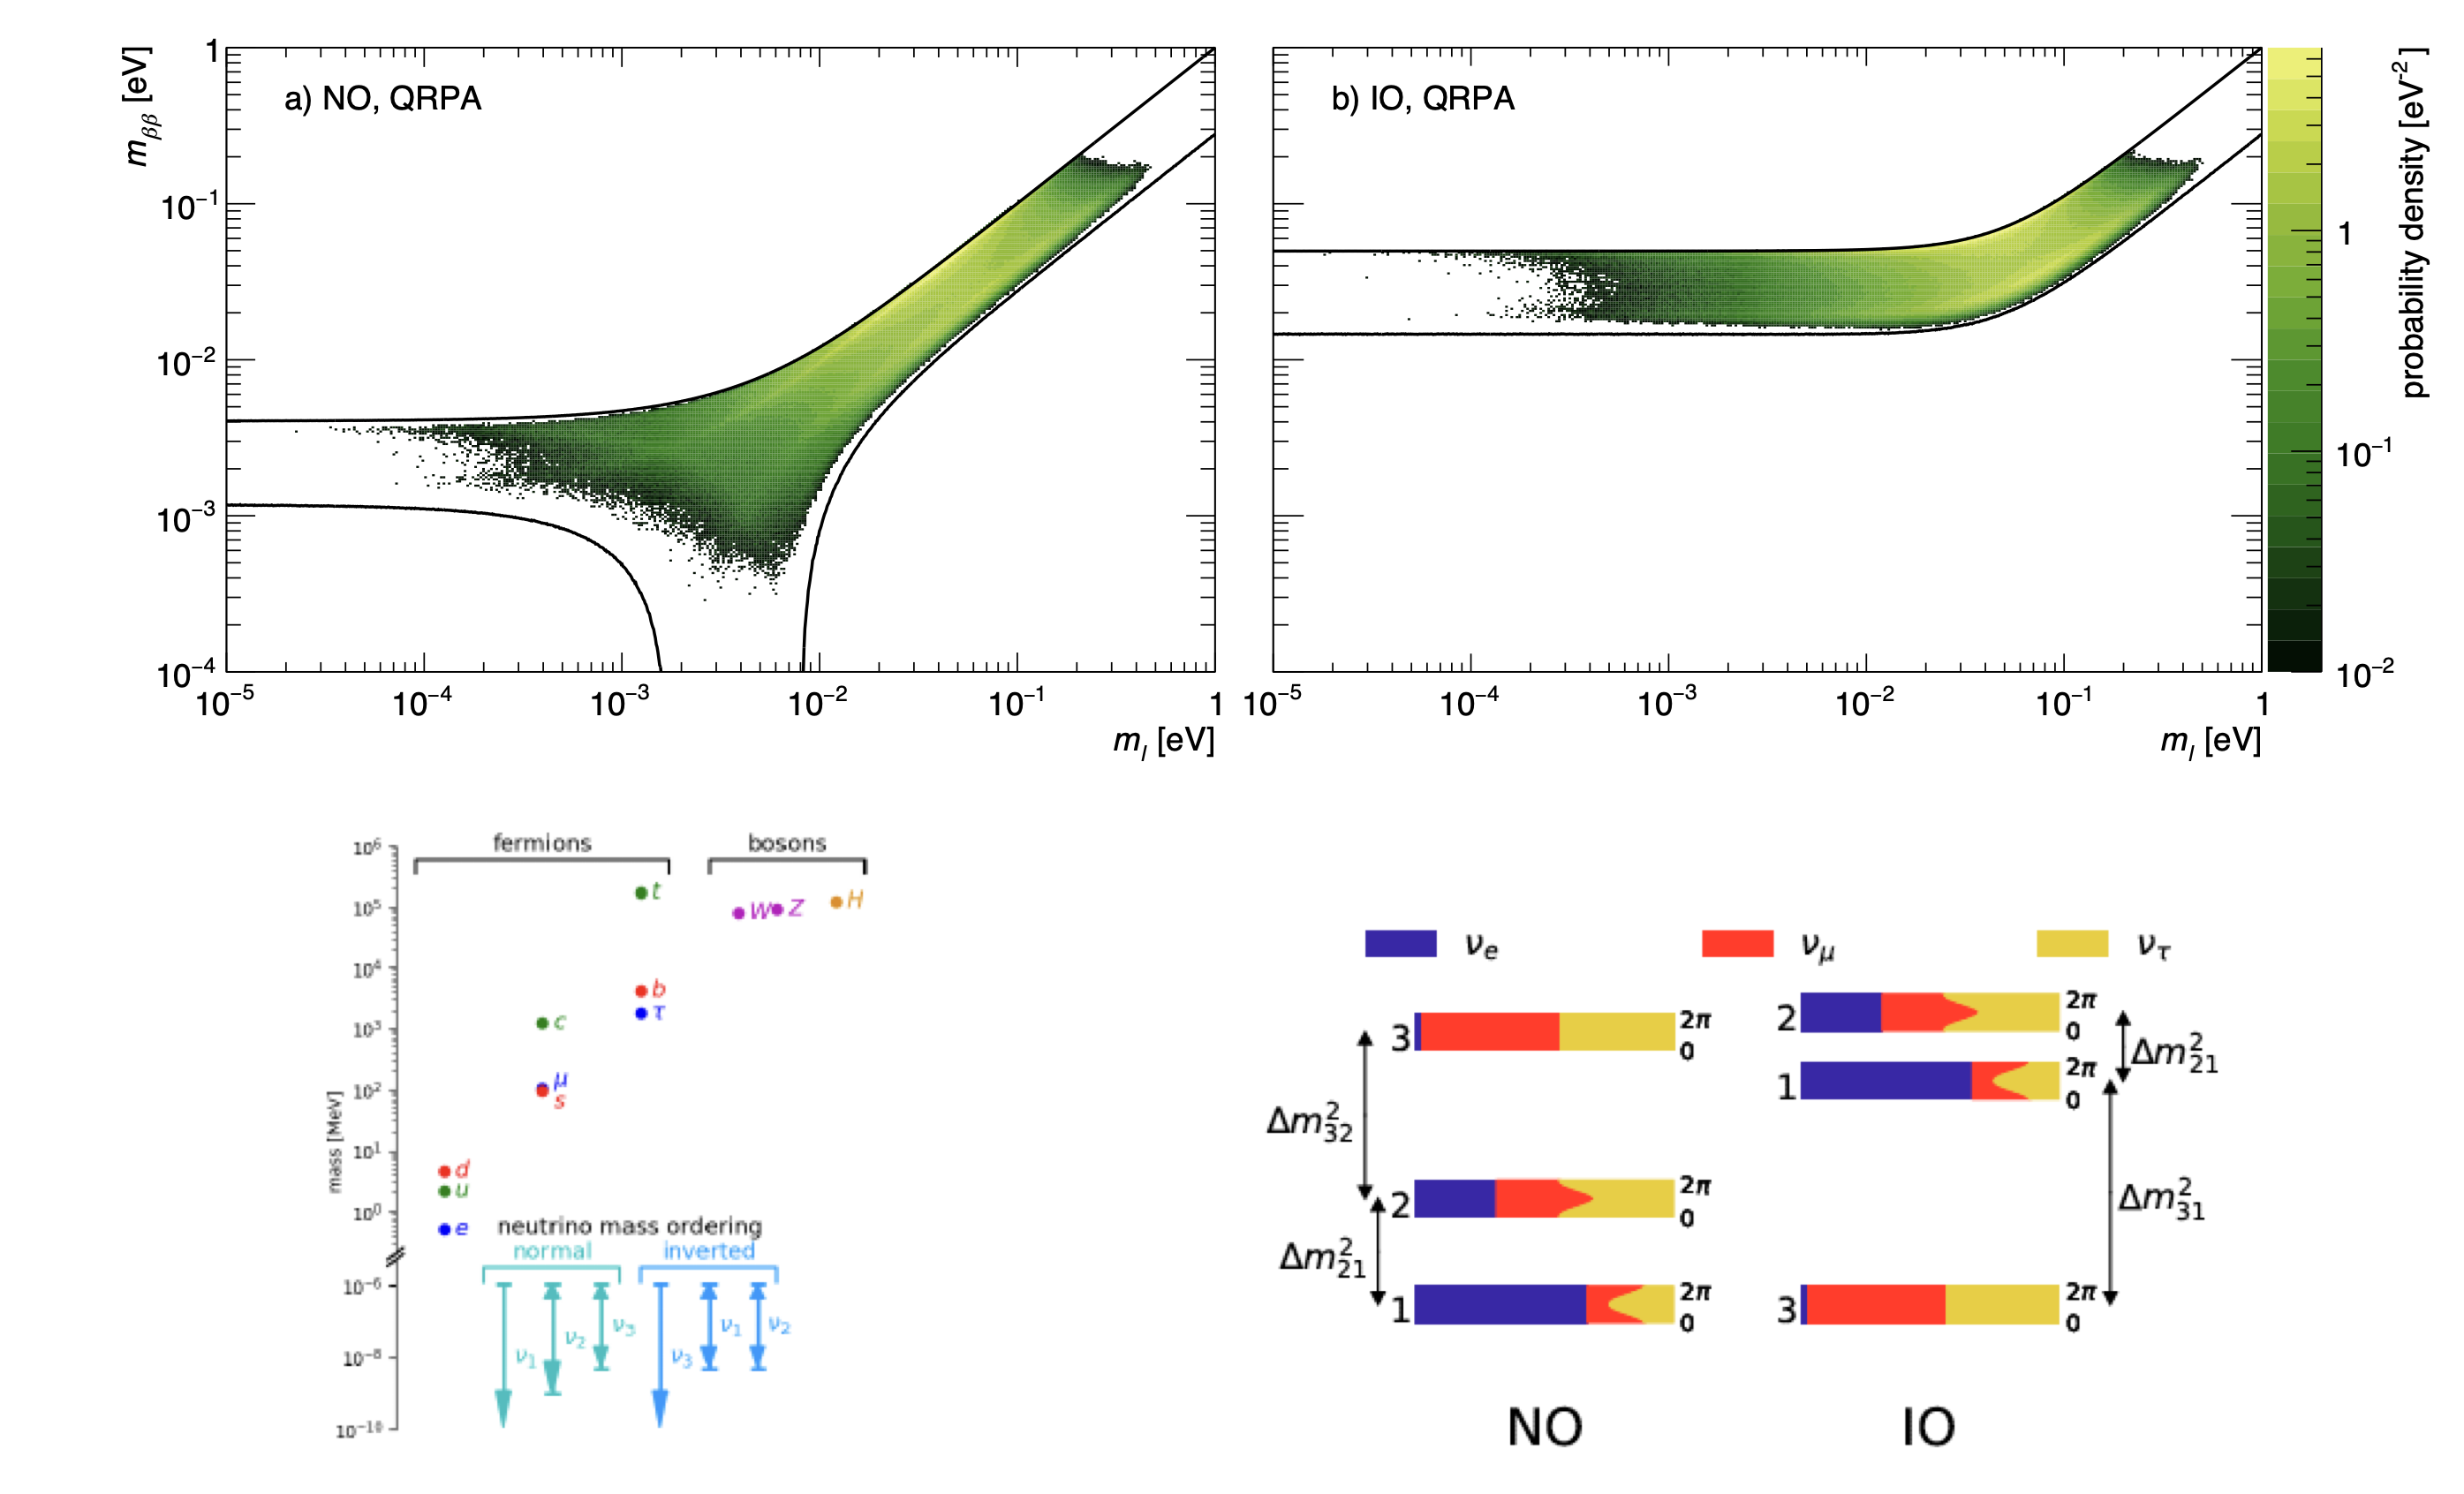
\includegraphics[scale=0.25]{landscape2.png}
\column{0.40\textwidth}

%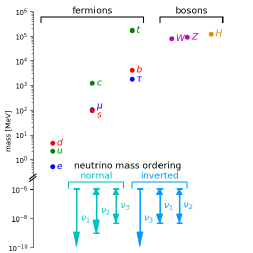
\includegraphics[scale=0.40]{ordering2.png}


%$\bullet~$ When representing $m_{\beta\beta}$~as a function of the mass of the lightest neutrino $m_l$, one obtains two possible landscapes, one for the ``Normal Ordering'' (NO) and the other for the ``Inverse Ordering" (IO). 
%
%$\bullet~$ Color shows probability. 
\end{columns}

\end{frame}
%%%

\begin{frame}{The challenge for $\beta\beta0\nu$ experiments}

\begin{columns}
\column{0.40\textwidth}
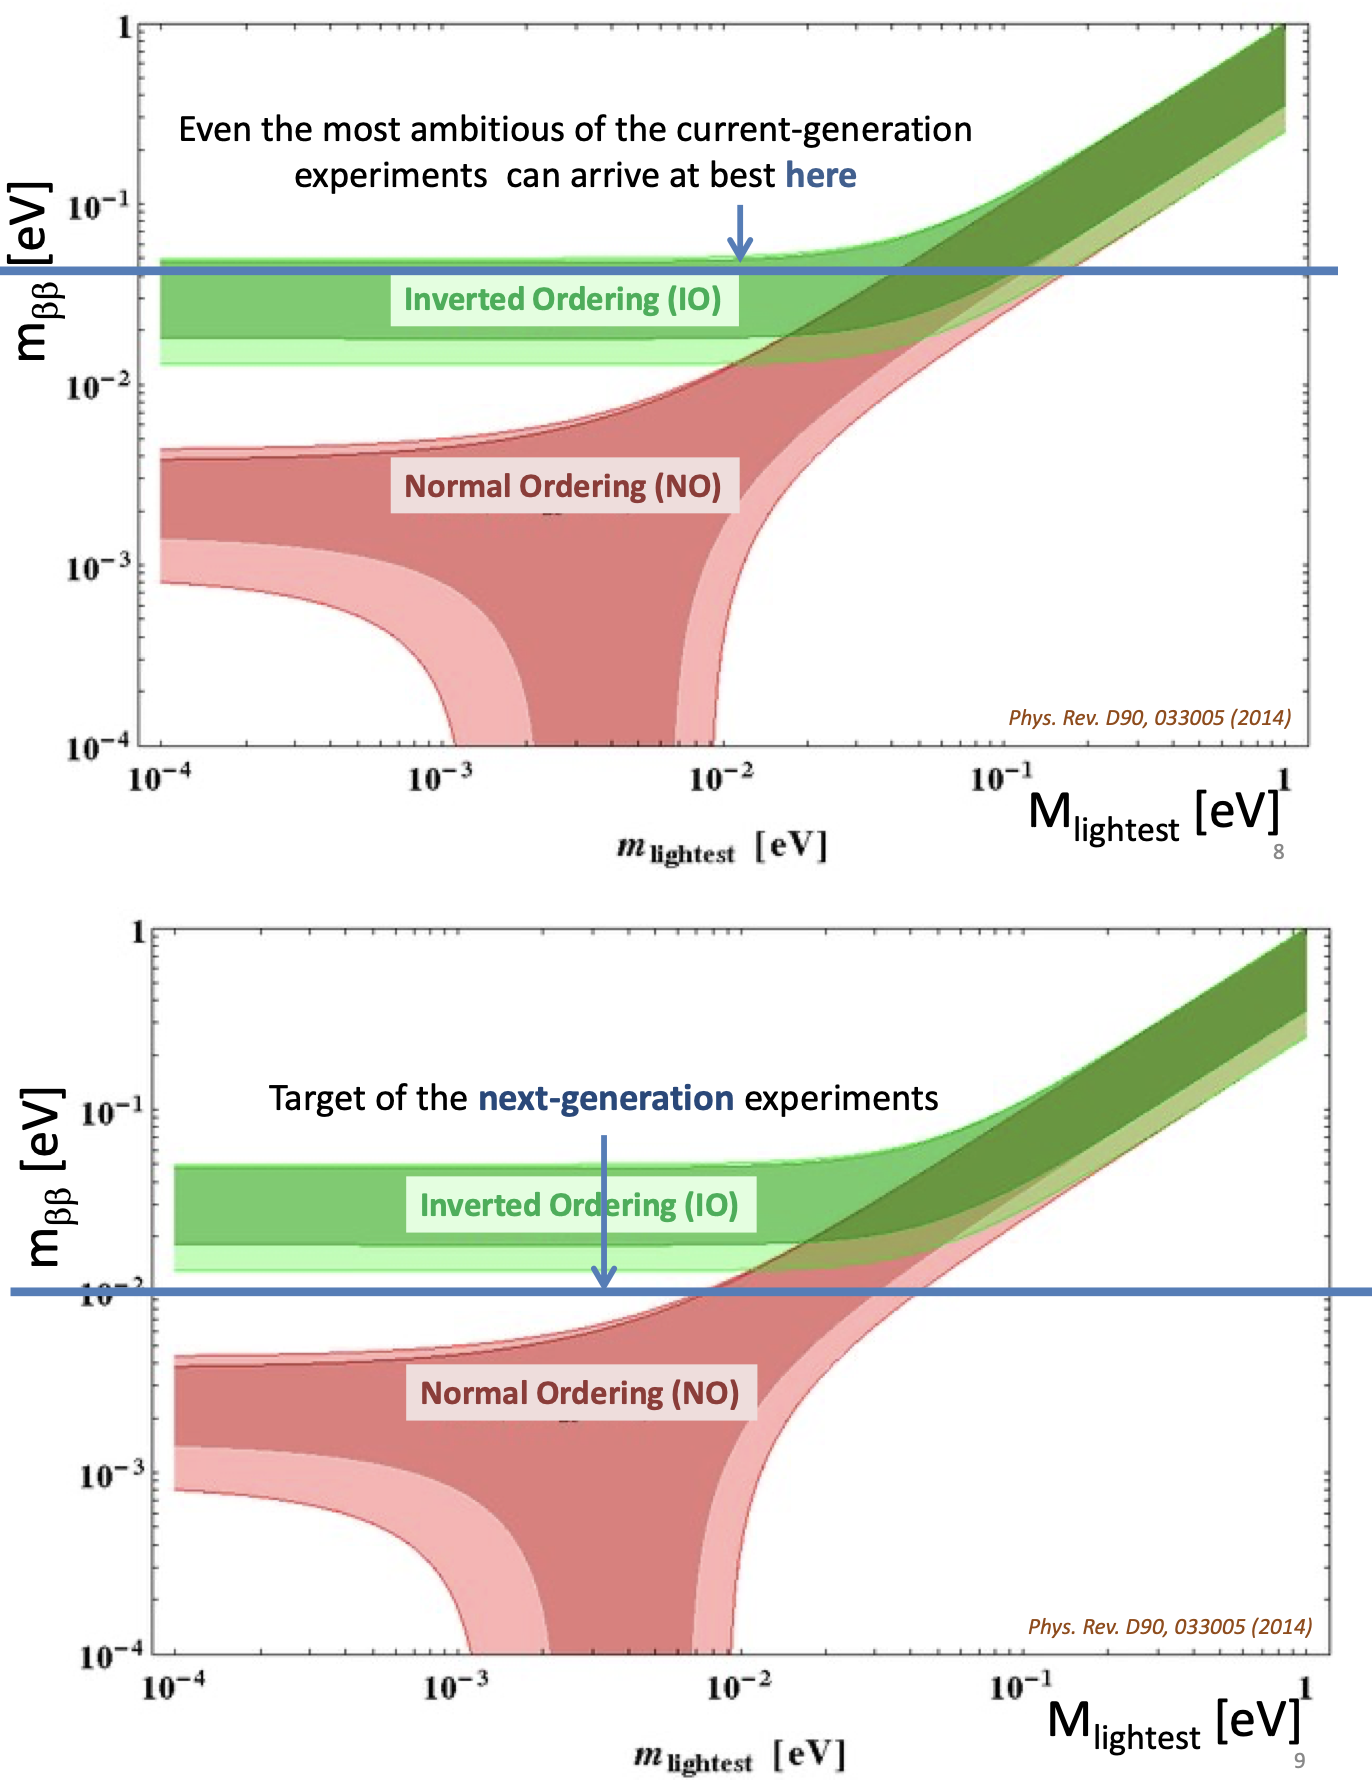
\includegraphics[scale=0.24]{landscapes.png}

 \column{0.60\textwidth}
 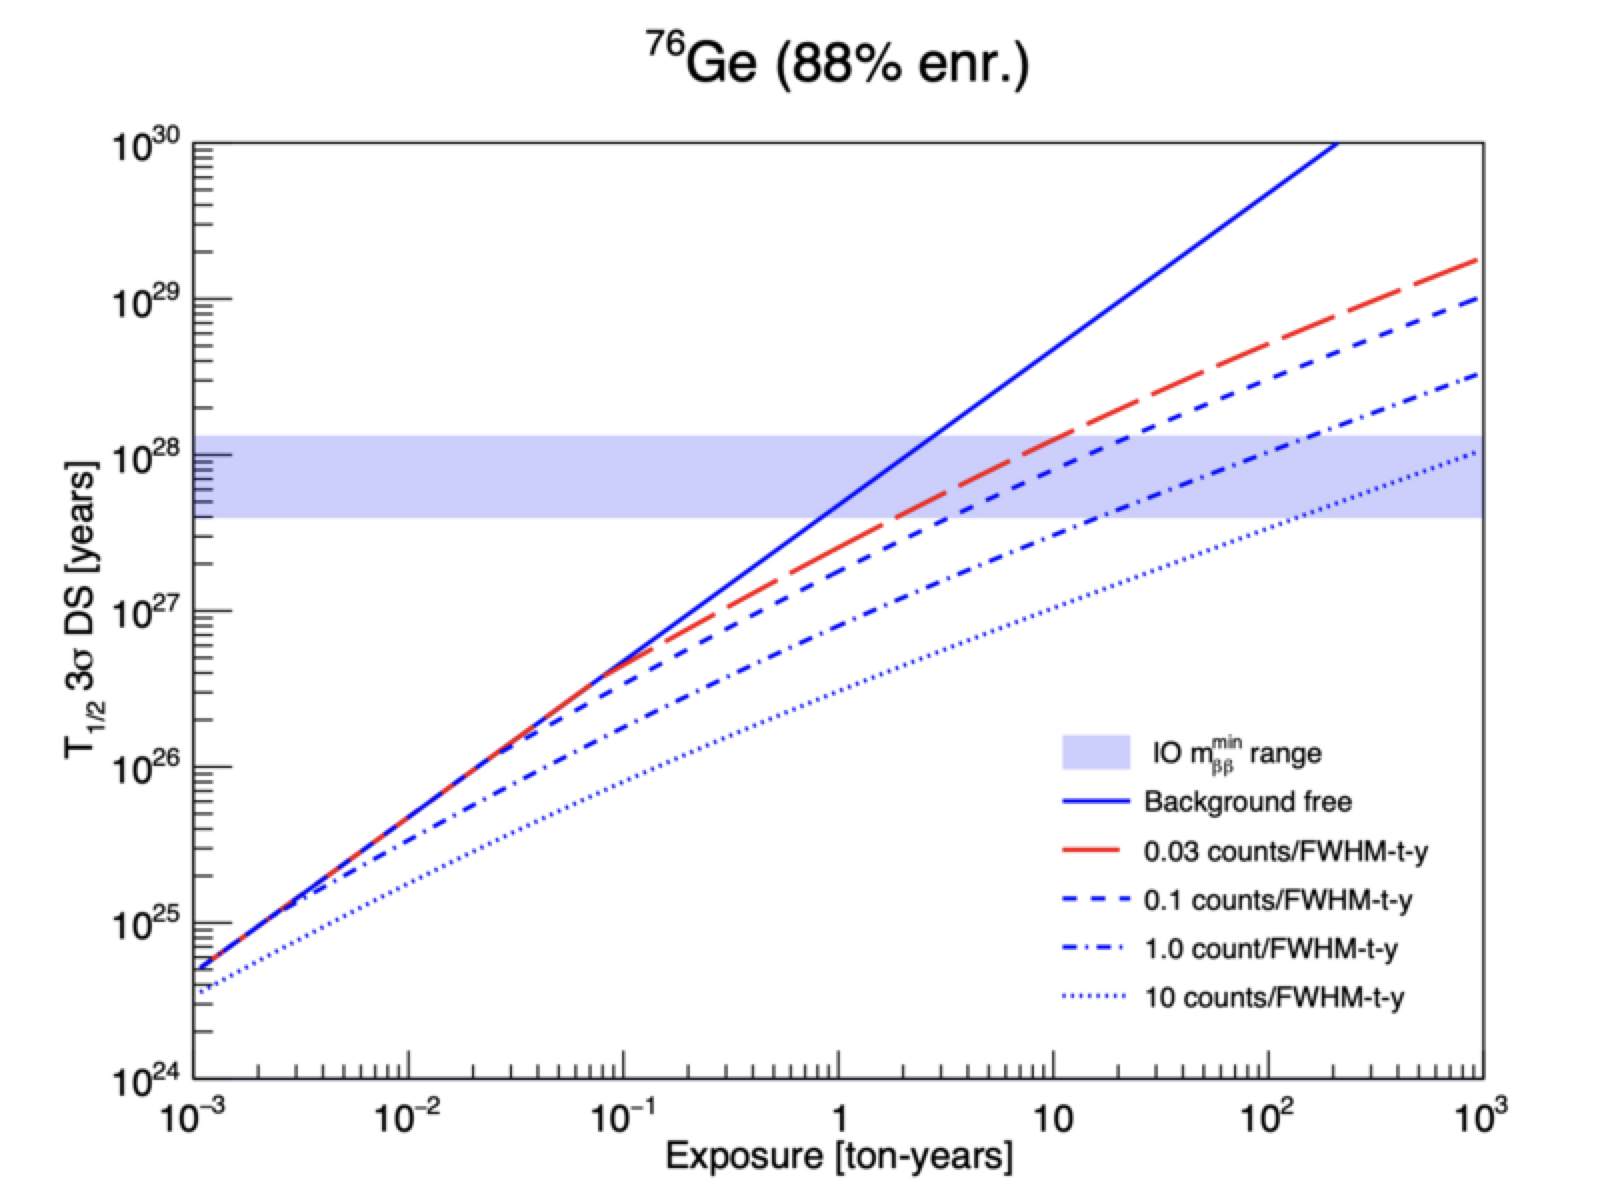
\includegraphics[scale=0.29]{ gesensi.png}
%$\bullet~$ Uncertainties in NME (exercise 2) translate in variations of almost one order of magnitude in expected lifetime (and thus expected rate) for a given $m_{\beta\beta}$. 
%
%$\bullet~$ Current generation of experiments have reached $4 \times 10^{26}$~y (KamLAND-Zen), which barely scrapes the IO, even in the most optimistic case. 
%
%$\bullet~$ Next generation of experiments target a sensitivity of $\sim 10^{27}$~y, which would cover IO only in the optimistic scenarios. 
%
%$\bullet~$ Next-to-next generation of experiments target a sensitivity of $\sim 10^{28}$~y, which would cover a fraction of the NO only in the optimistic scenarios. 
\end{columns}
\end{frame}

%%%%



%%%%

%\begin{frame}{${\beta\beta0\nu}$ signatures}
%
%\begin{columns}
%\column{0.40\textwidth}
%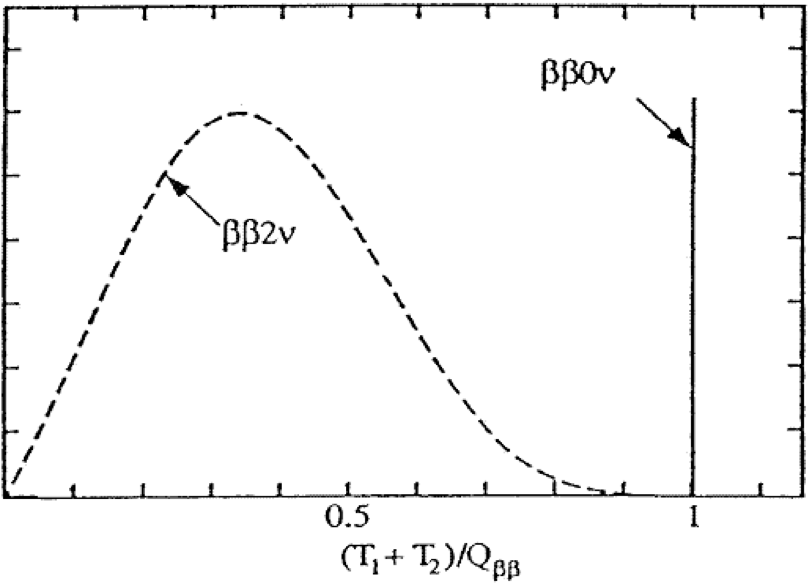
\includegraphics[scale=0.43]{idealdet.png}
%
%
% \column{0.60\textwidth}
% 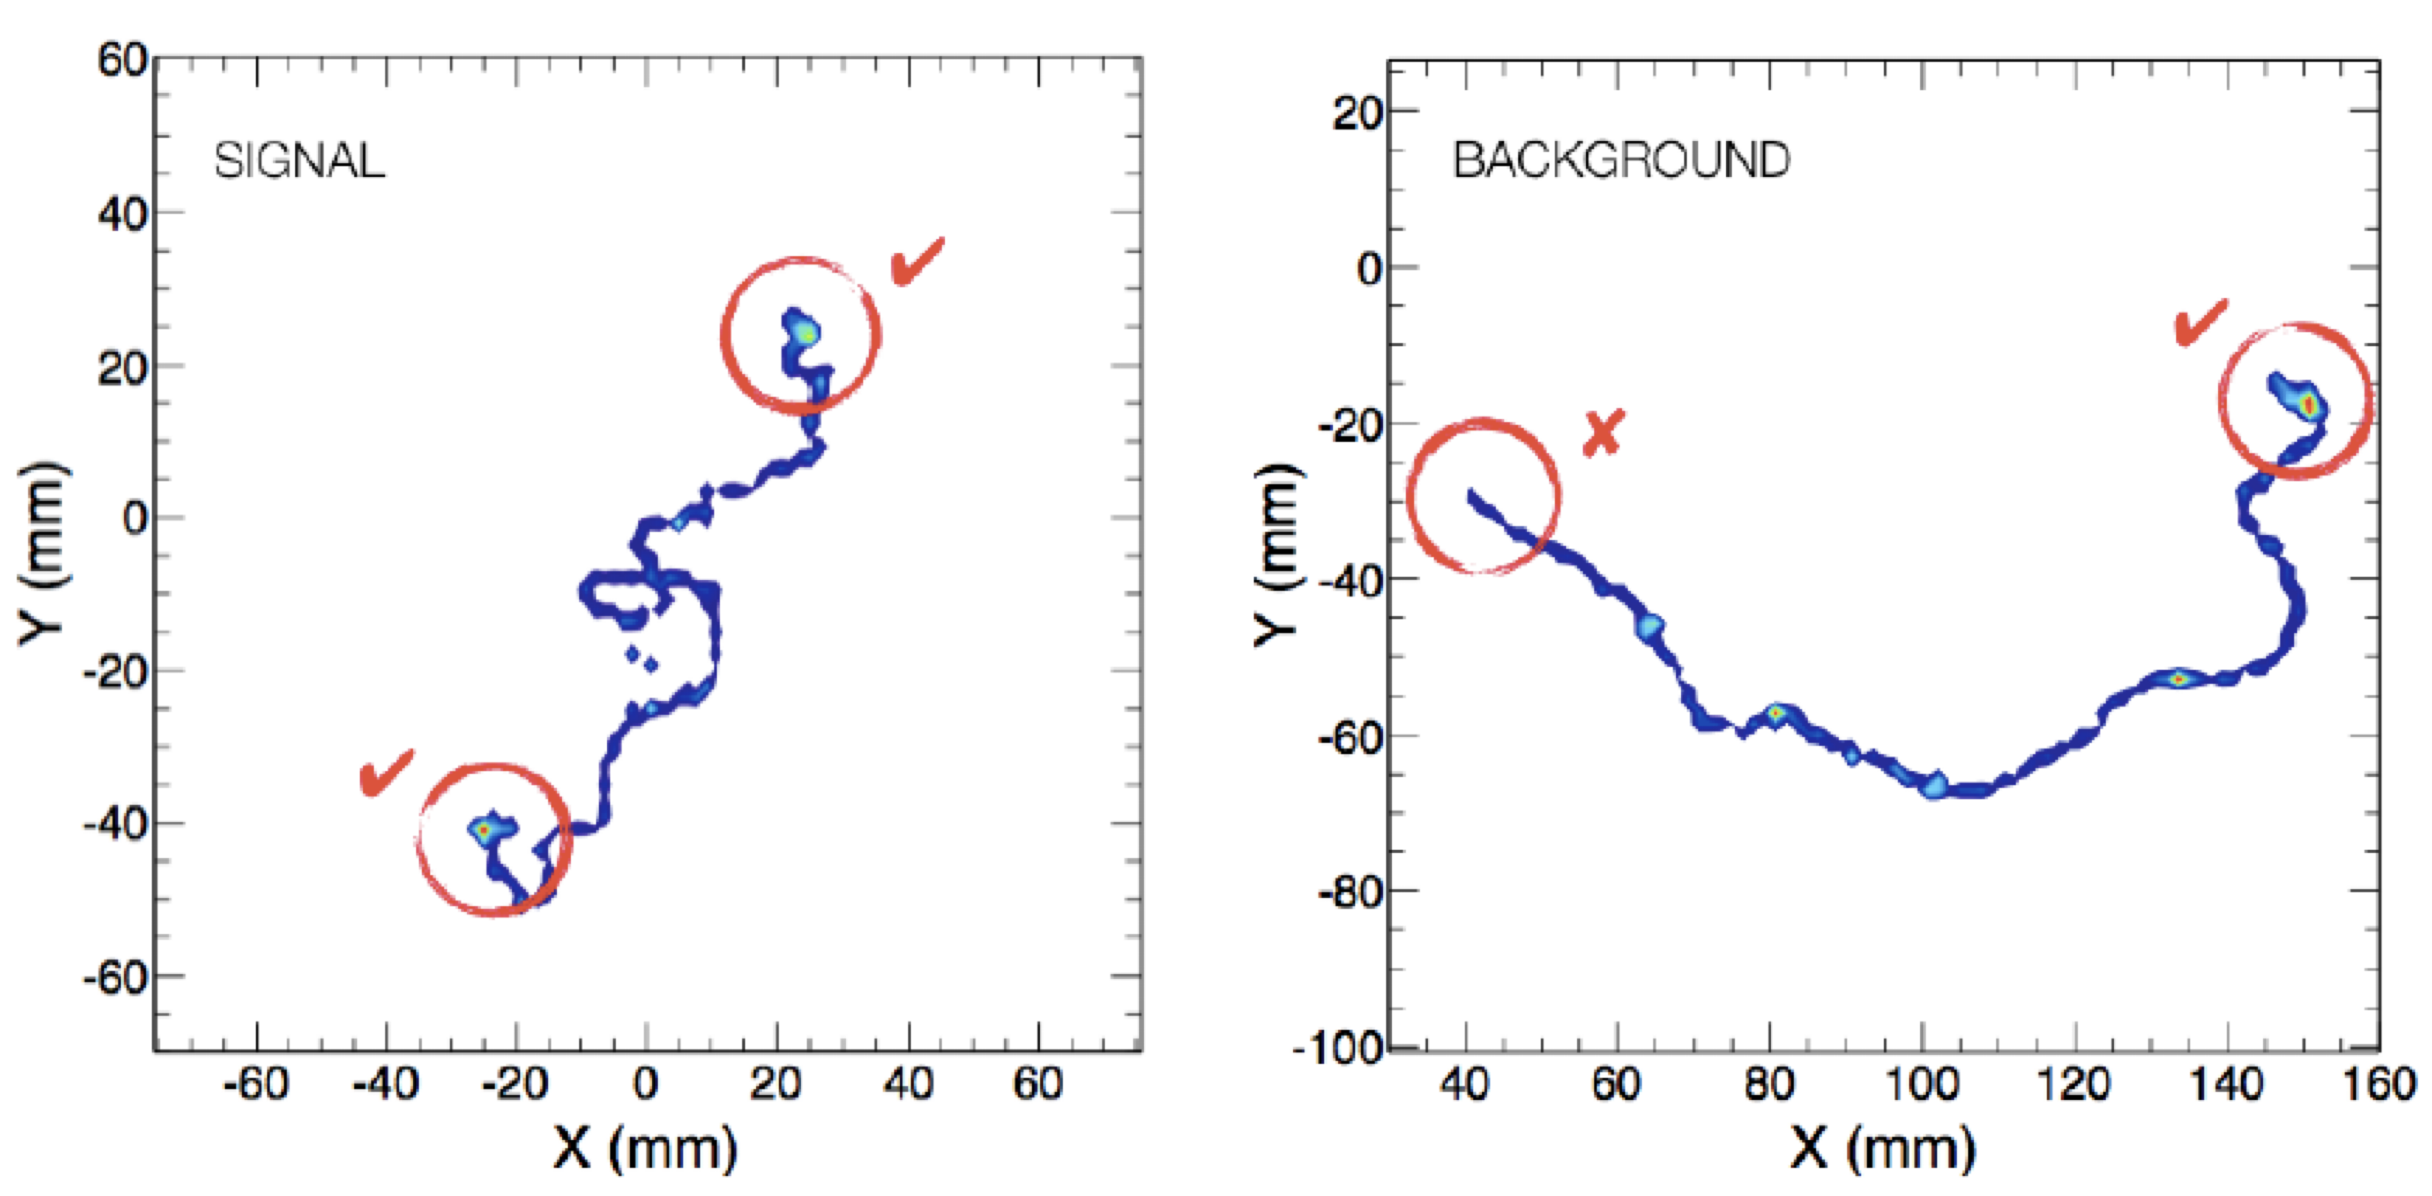
\includegraphics[scale=0.19]{idealtopo.png}
%$\bullet~$ Get yourself a detector with {\em perfect energy resolution}. 
%
%$\bullet~$ Measure the energy of the emitted electrons and select those with 
%$(T_1+T_2)/Q_{bb} = 1$.
%
%$\bullet~$ Do not worry about backgrounds, a detector with perfect energy resolution suppresses them all. 
%
%$\bullet~$ Count the number of observed events (they are all signal) and calculate the corresponding lifetime.

%\end{columns}
%\end{frame}

%%%%

%\begin{frame}{\XE\ is a good isotope for \bbonu\ searches}
%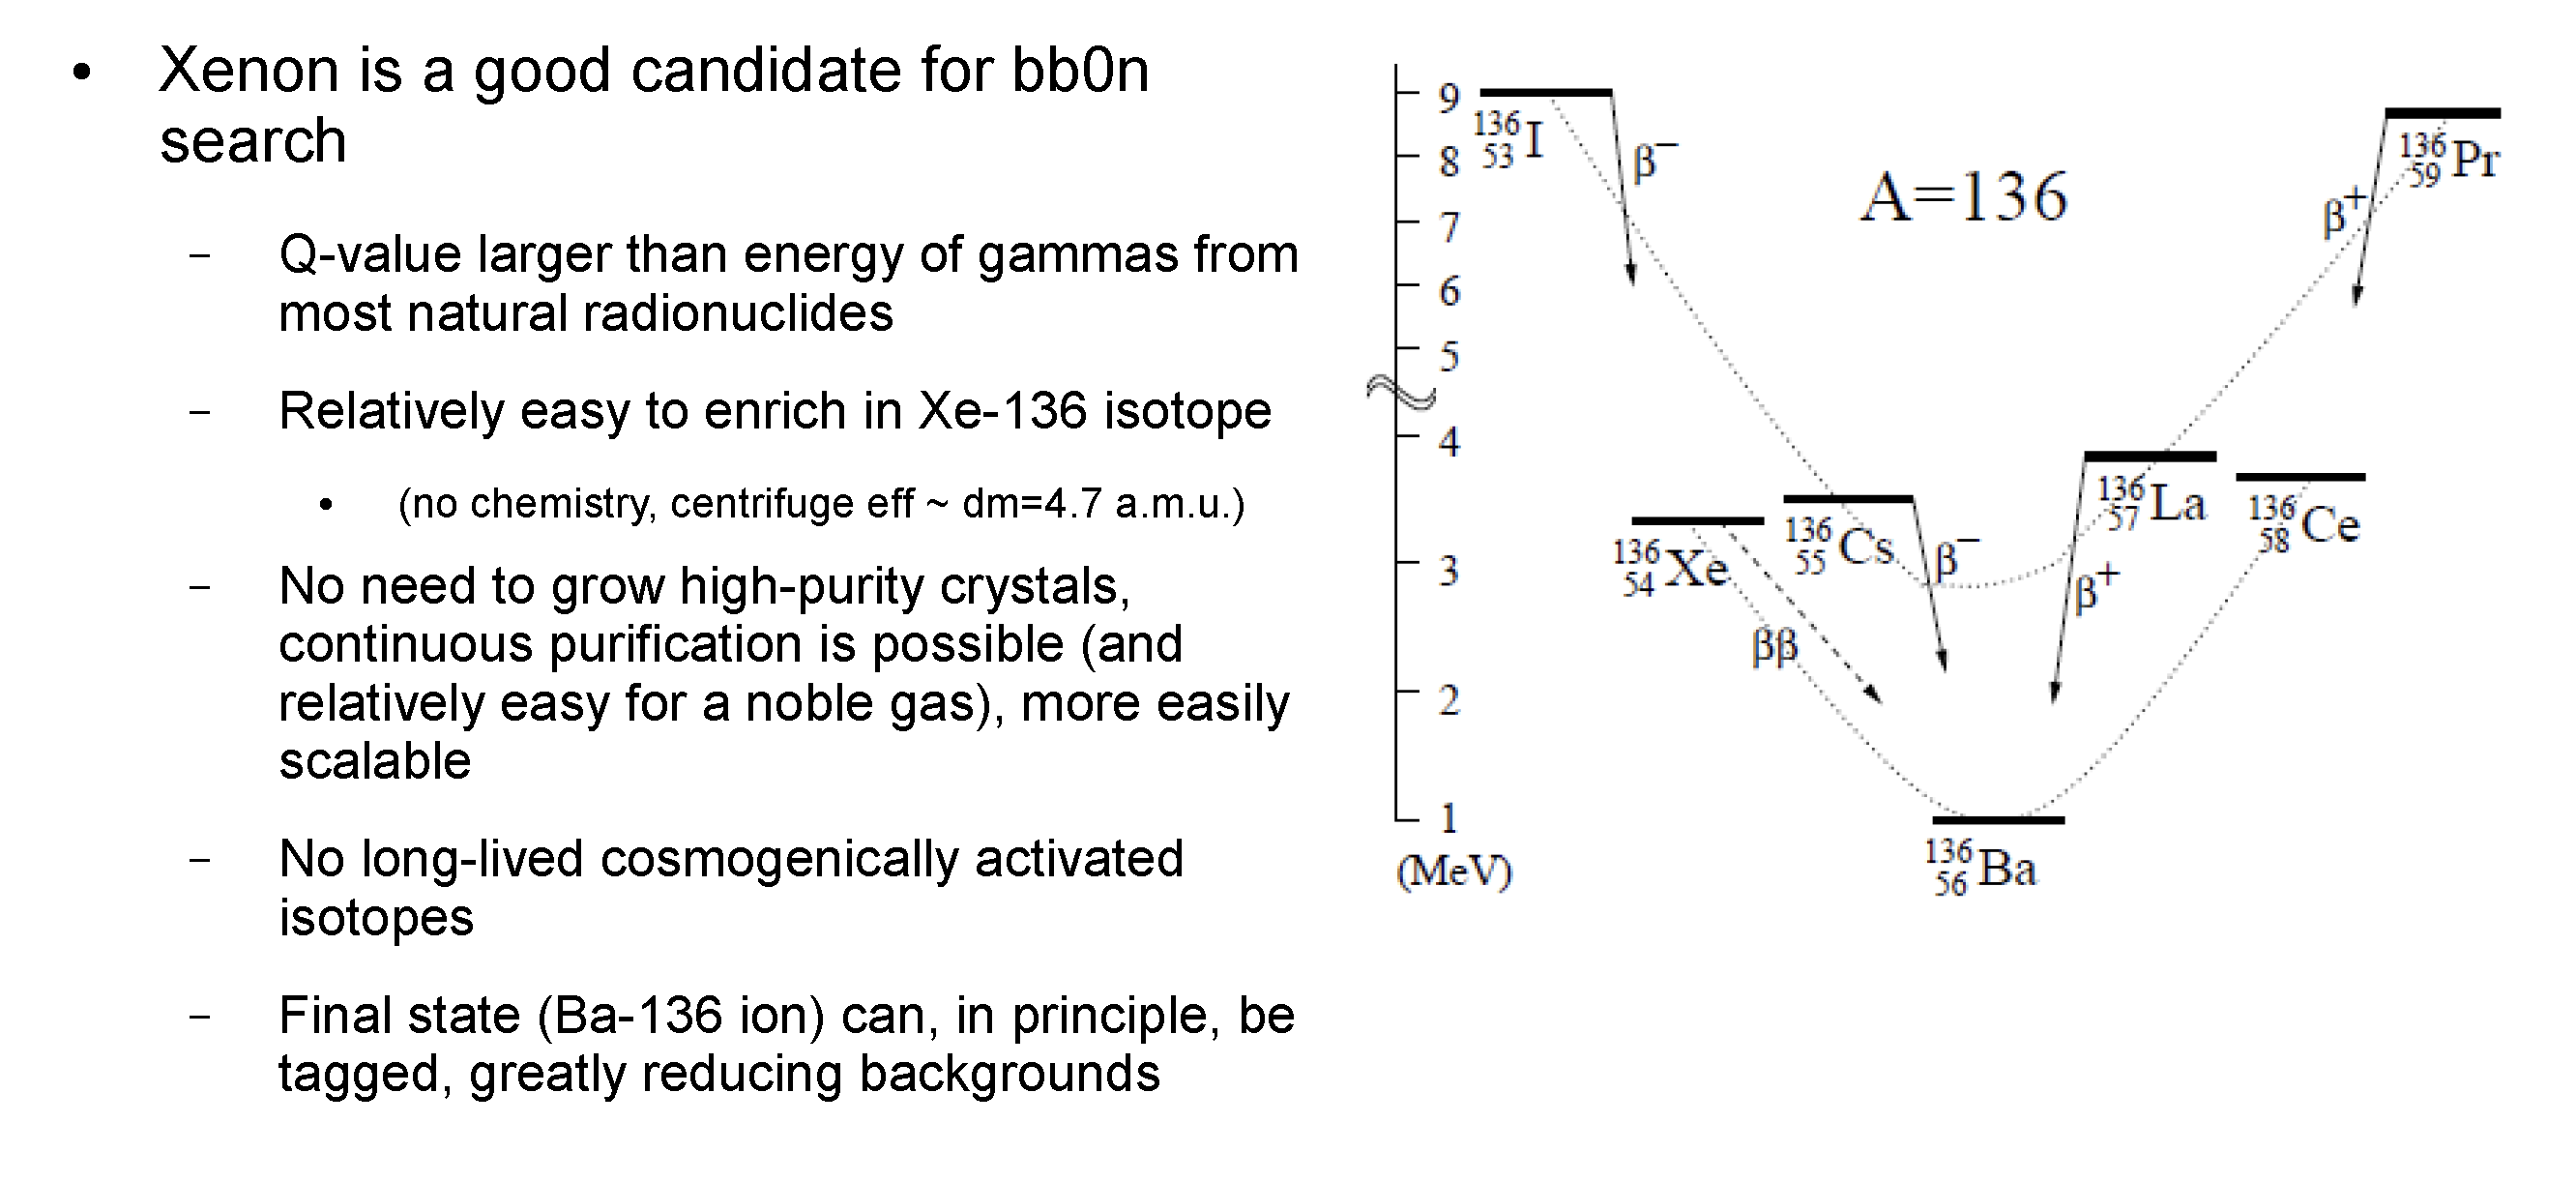
\includegraphics[scale=0.42]{xenonbbonu2.png}
%\end{frame}
%
%\begin{frame}{The NEXT concept: A HPXe EL TPC}
%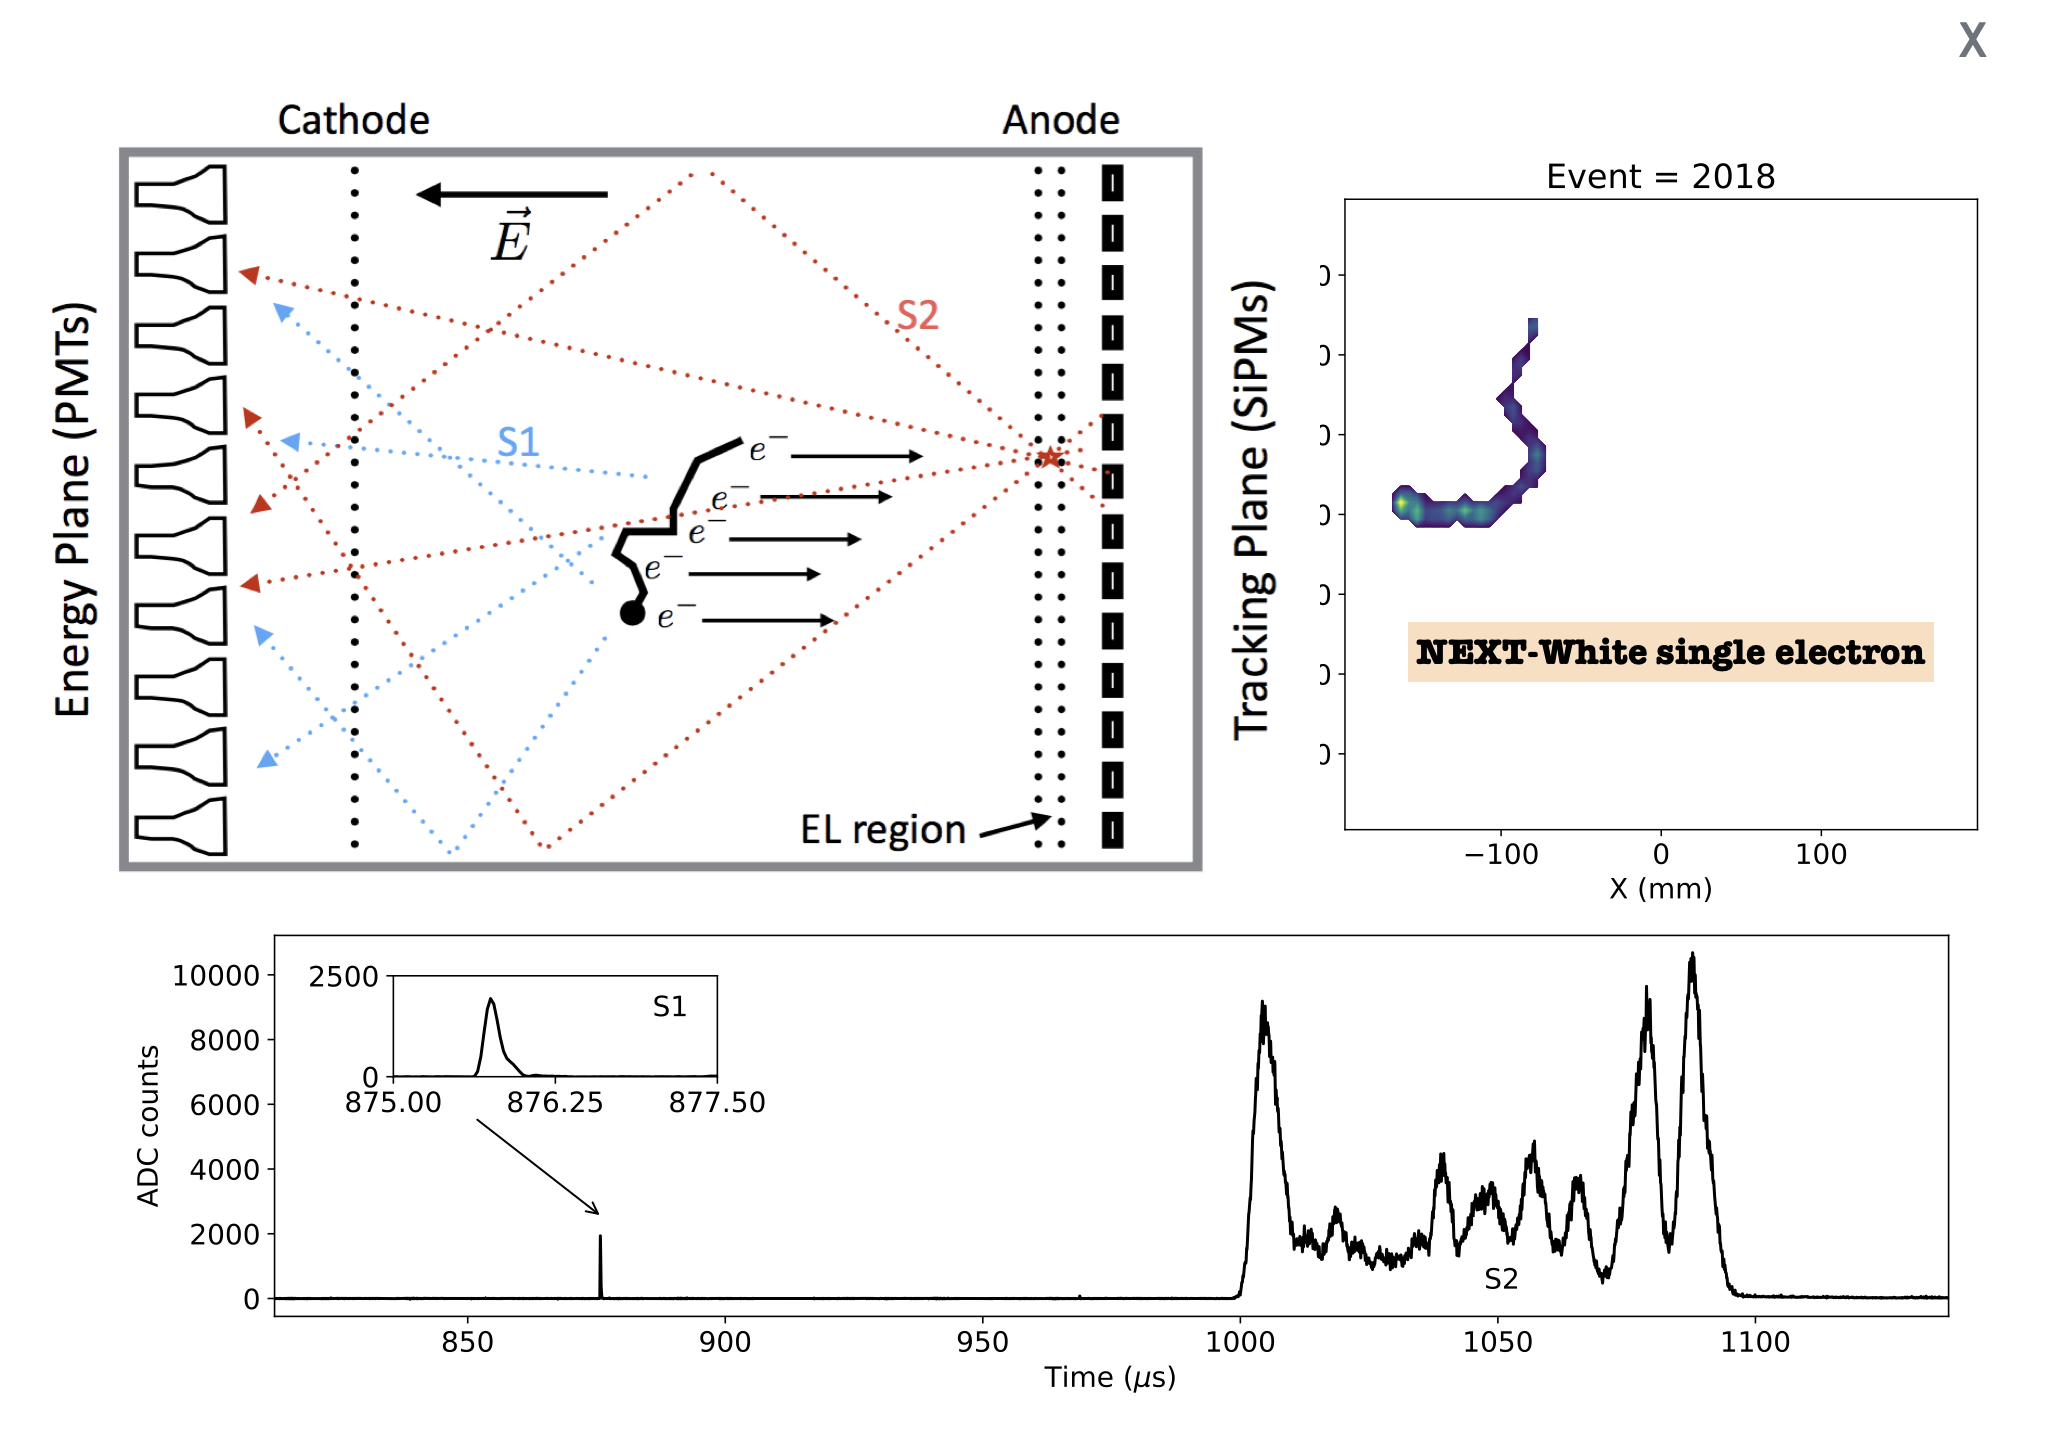
\includegraphics[scale=0.30]{nextpo.png}
% 
%\end{frame}


%%%%%
\begin{frame}{Principle of operation of a HPXe EL TPC}

%\begin{figure}[htb!]
%\centering
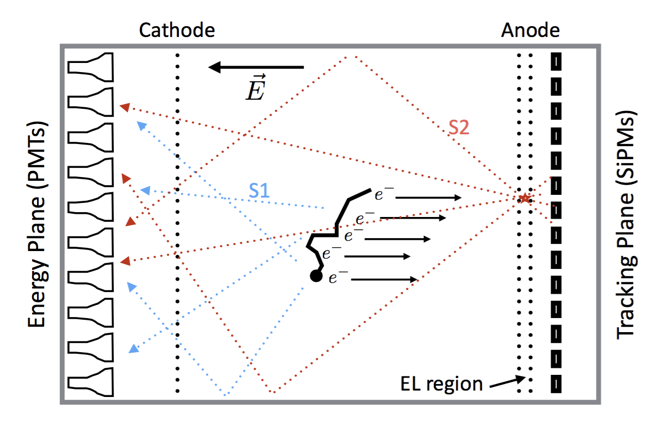
\includegraphics[width=0.45\textwidth]{PrincipleOfOperation.png}
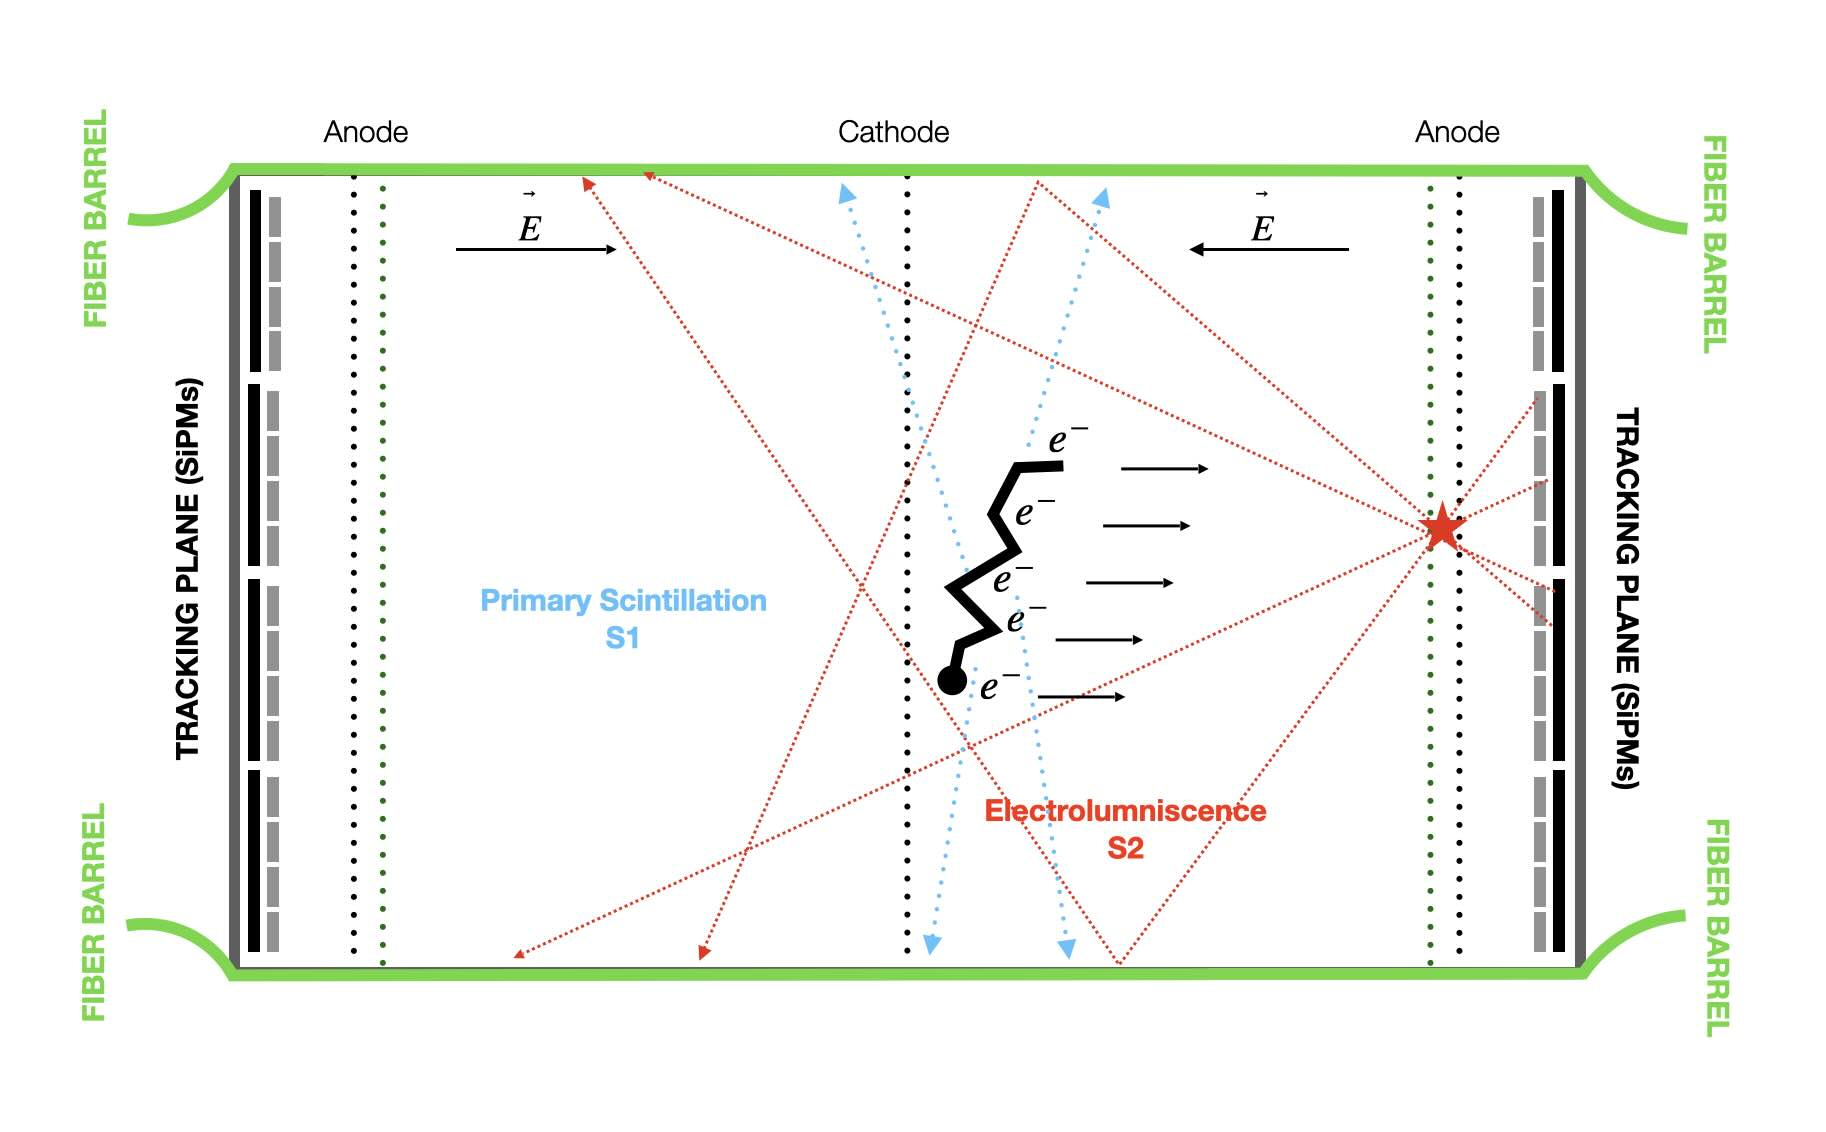
\includegraphics[width=0.50\textwidth]{symetric.jpeg}
% Symmetric
%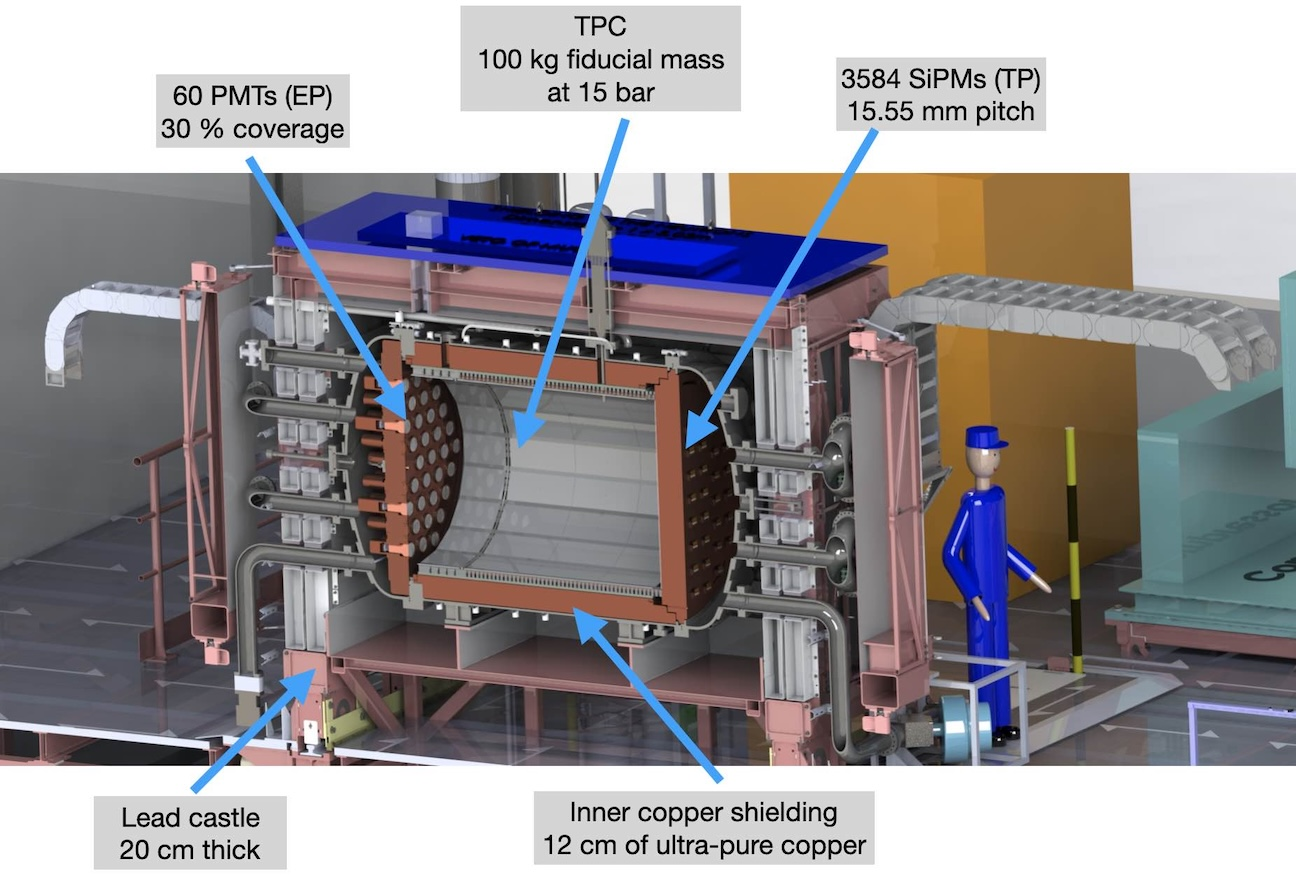
\includegraphics[width=0.5\textwidth]{img2/NEXT-100-description.jpg}
%\includegraphics[width=0.50\textwidth]{Next100.jpeg}
%\vspace*{-2mm}
%\caption{Principle of operation of a HPXe EL TPC. Left panel: asymmetric TPC. Right panel: symmetric TPC.}
%\label{fig:hpxe}
%\end{figure}

\end{frame}

%%
\begin{frame}{NEXT-100}

\begin{columns}
\column{0.60\textwidth}
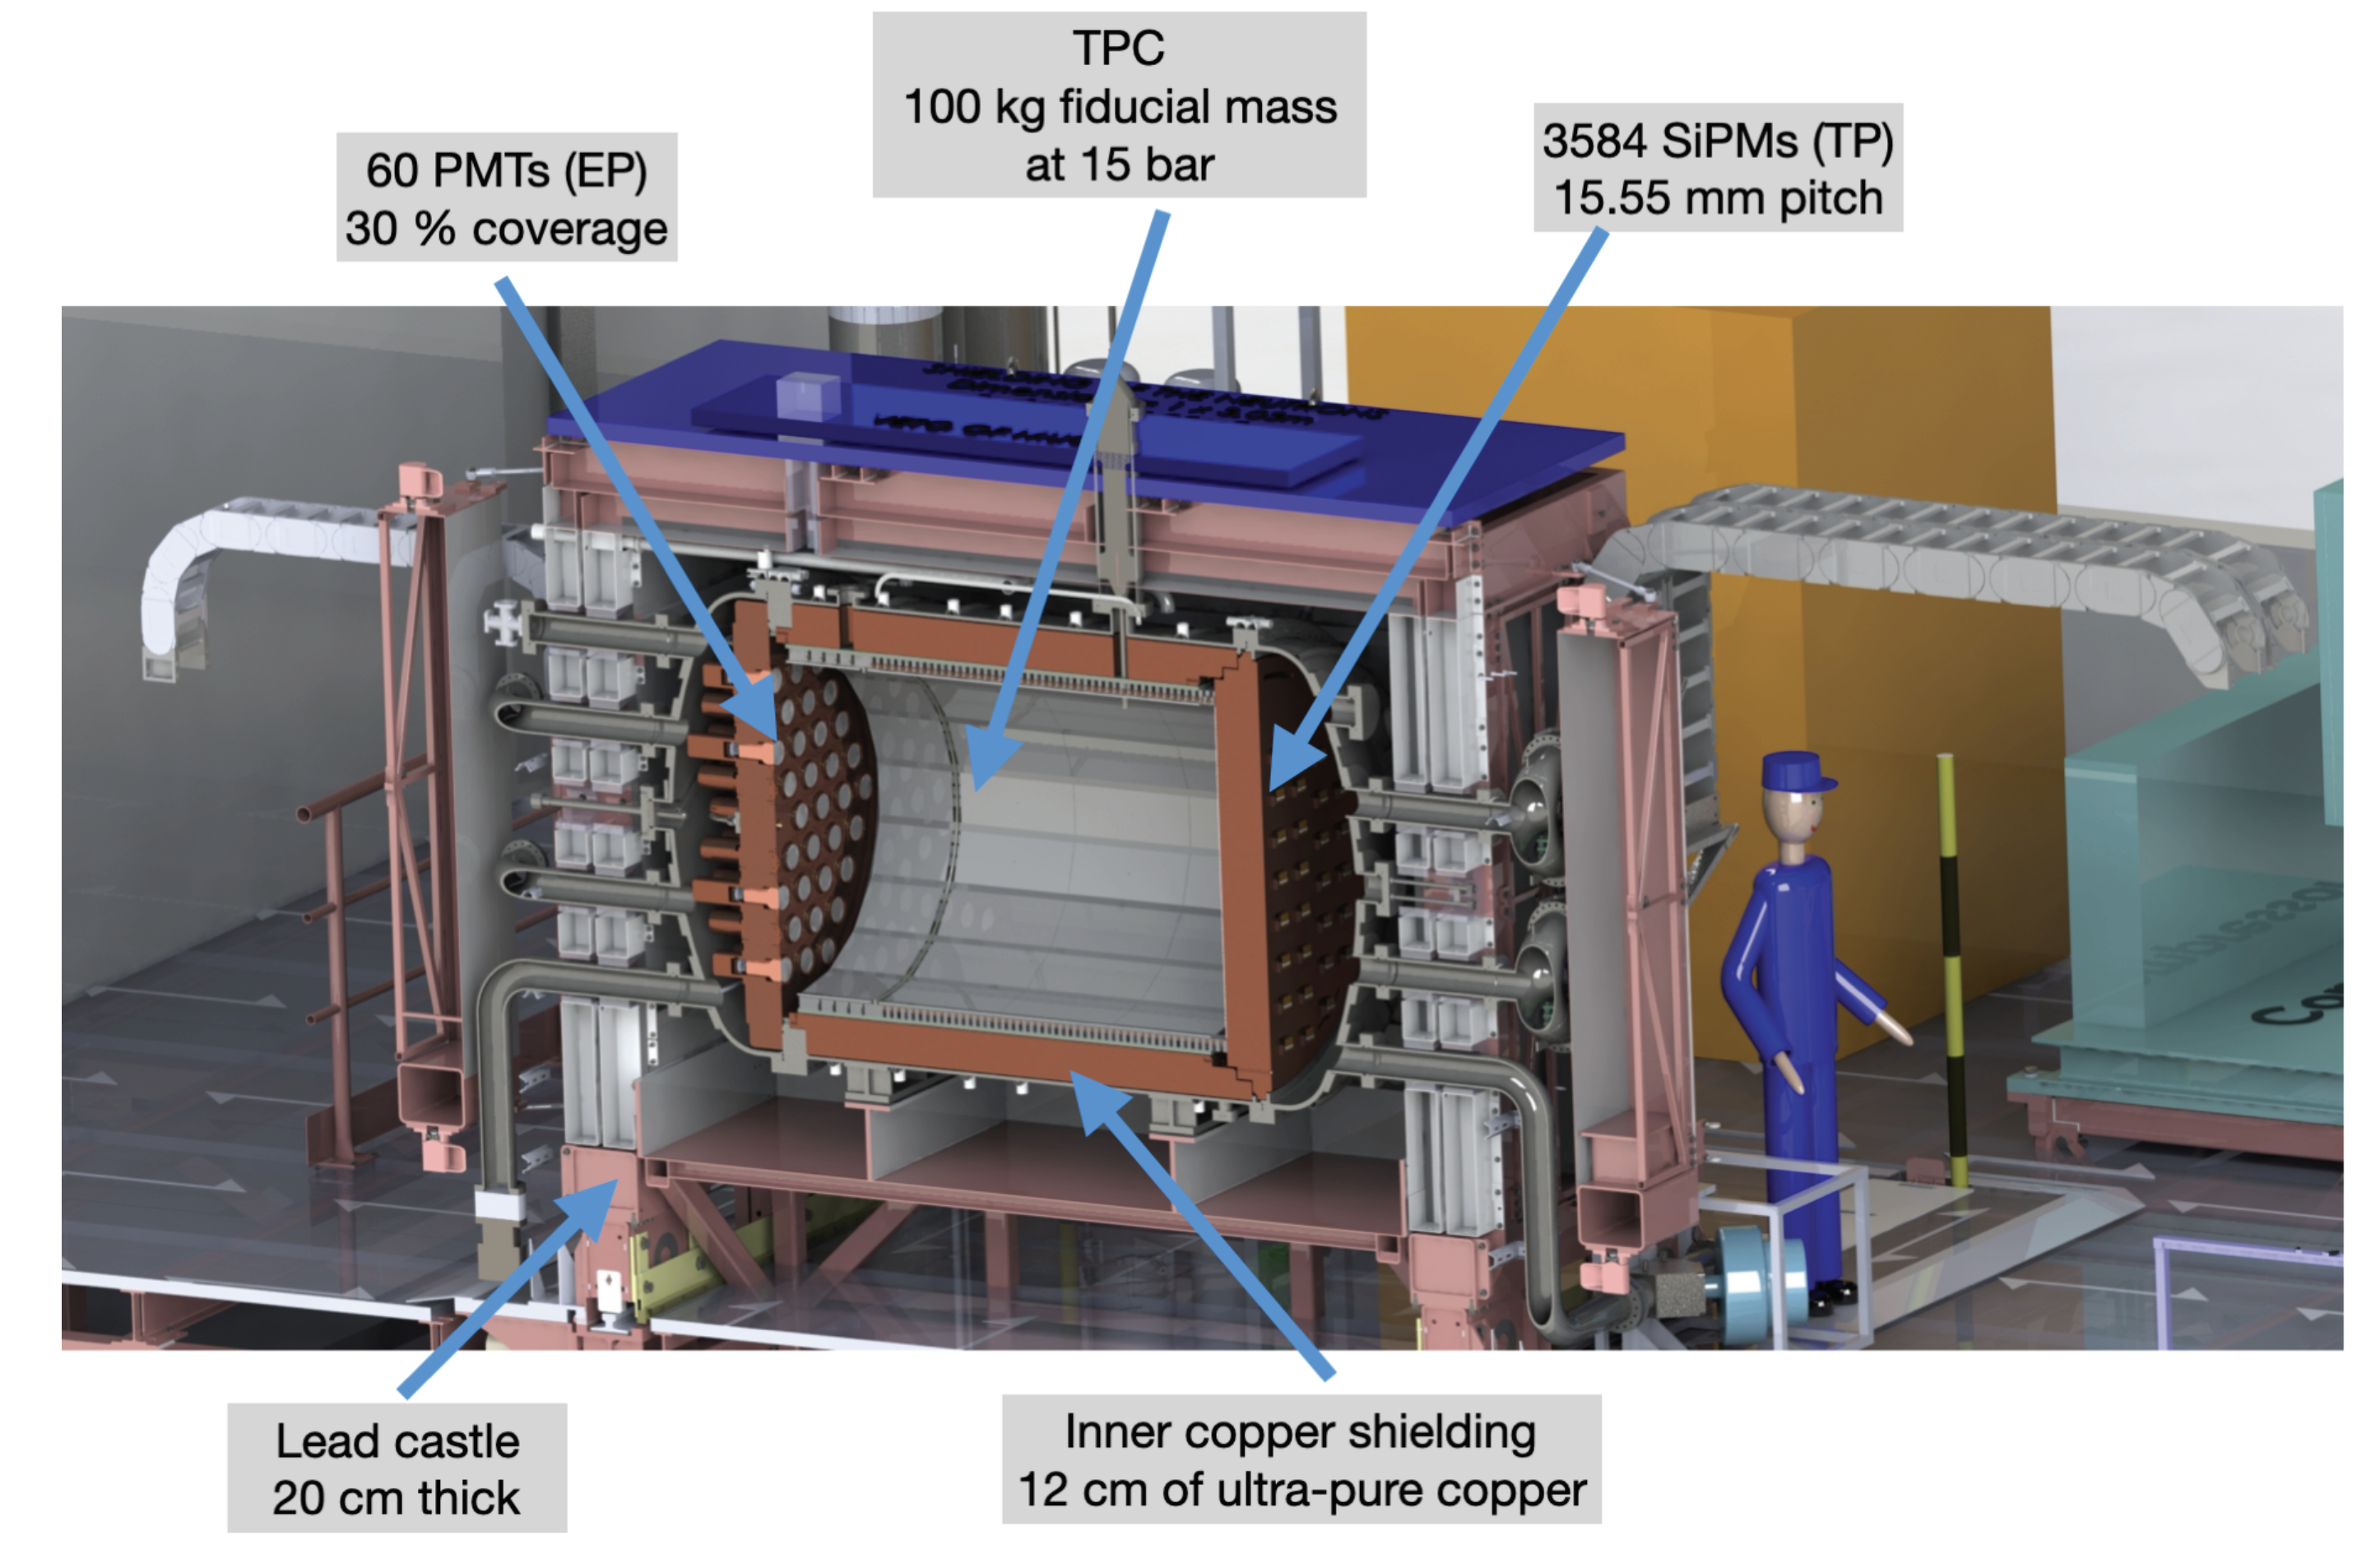
\includegraphics[scale=0.24]{next100withcastle.png}


 \column{0.40\textwidth}
$\bullet~$ NEXT-100 is operating at LSC since 2024. Holds 100 kg of xenon enriched at 90\% in \XE\ (at 15 bar). 

\end{columns}
\end{frame}


\begin{frame}{NEXT-100 main components}
\begin{columns}
\column{0.50\textwidth}

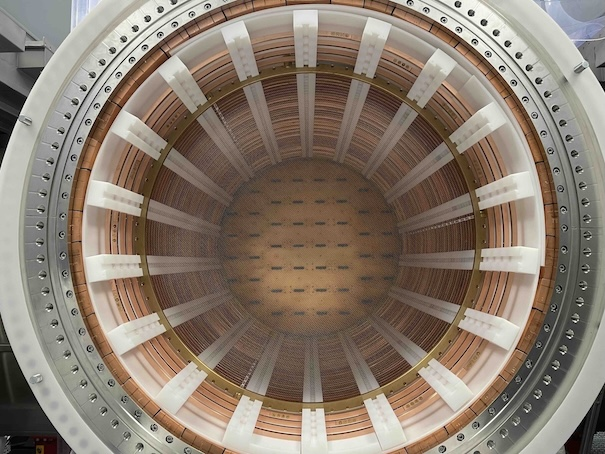
\includegraphics[width=0.90\textwidth]{n100-tpc.jpeg}

\vspace*{5mm}


 \column{0.50\textwidth}
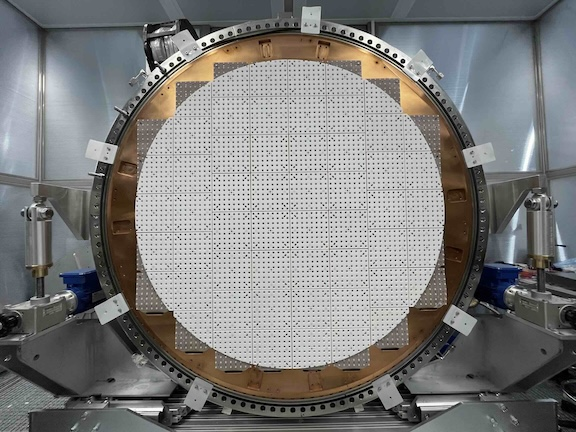
\includegraphics[width=0.60\textwidth]{n100-tp.jpeg}

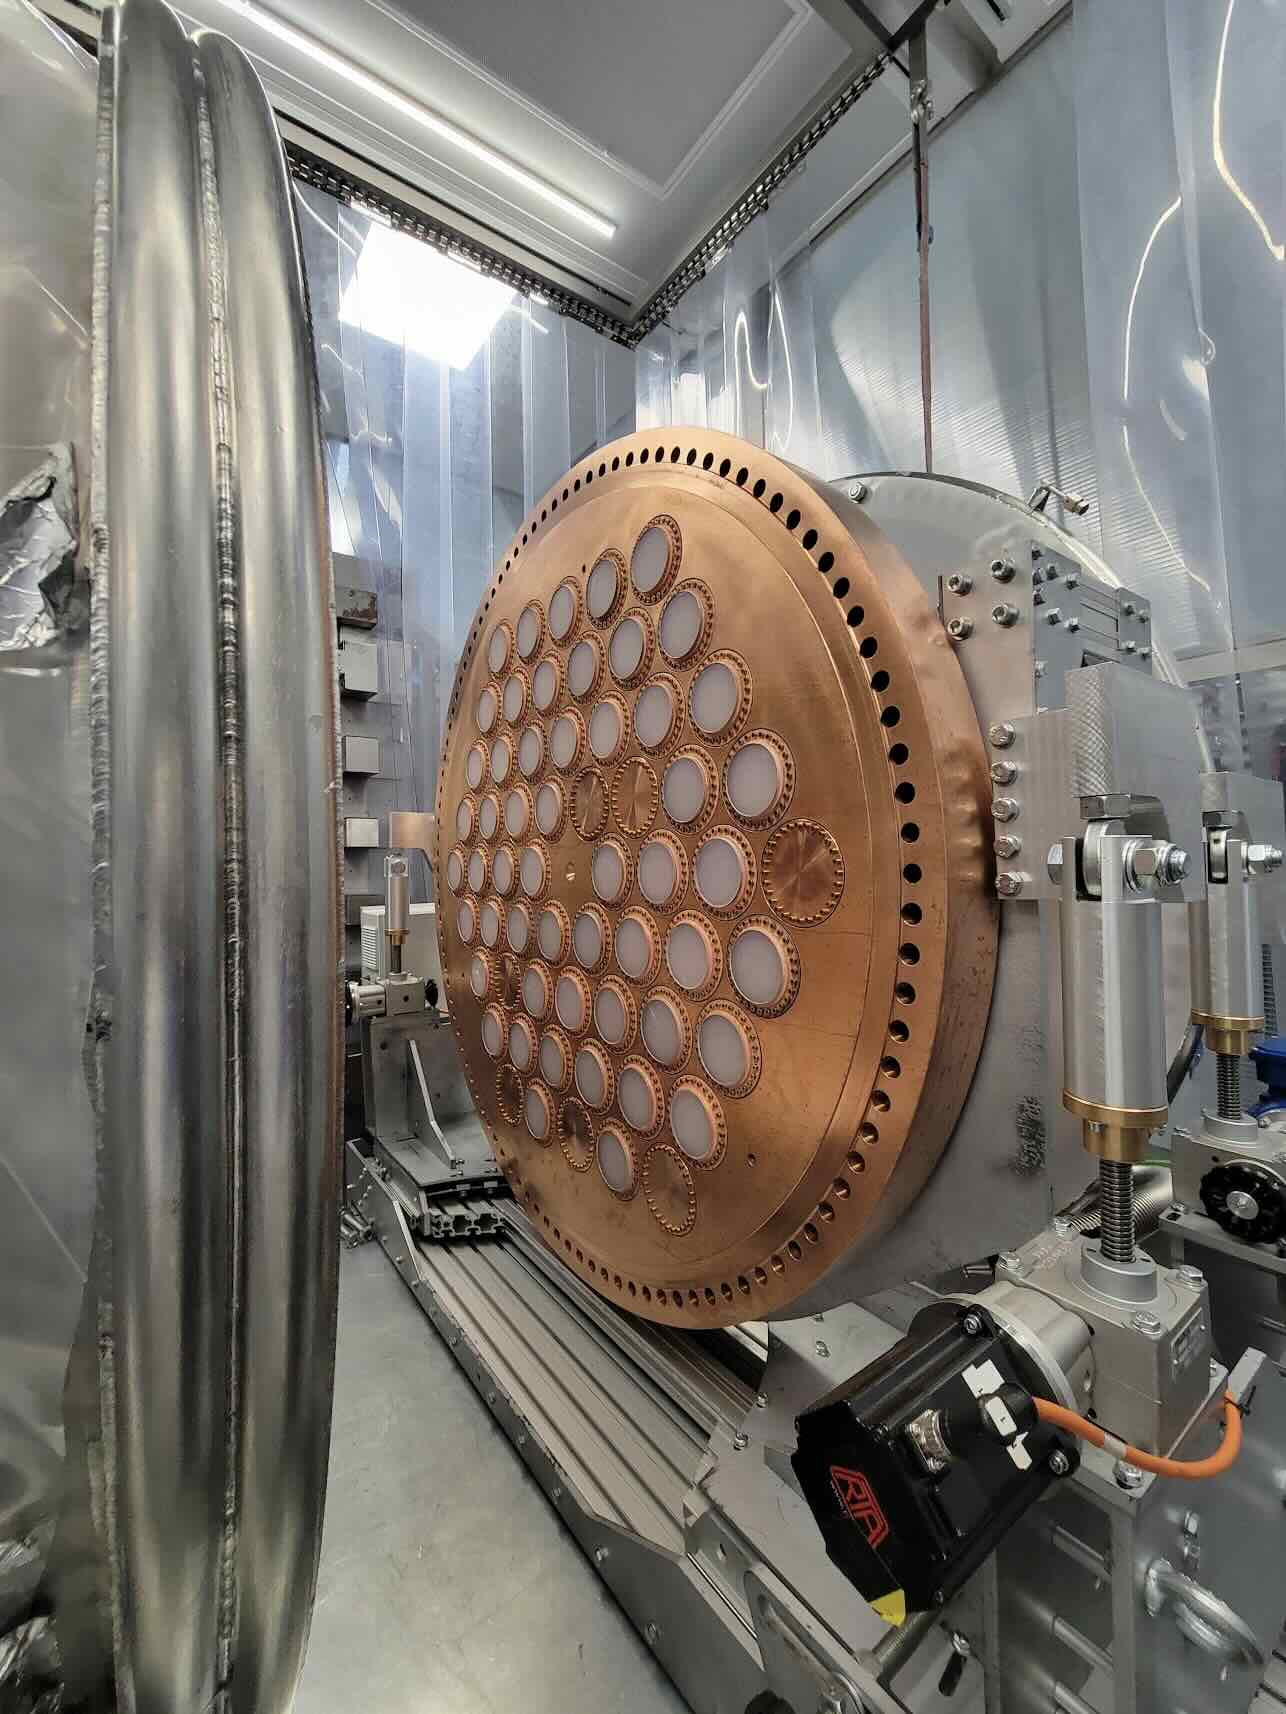
\includegraphics[width=0.60\textwidth]{n100-pmt.jpeg}

\end{columns}
\end{frame}


\begin{frame}{Pressure Vessel}

\includegraphics[scale=0.23]{next100pv.png}

\end{frame}

%%%
\begin{frame}{Inner Copper Shield}

\includegraphics[scale=0.23]{innercopper.png}

\end{frame}

%%
\begin{frame}{Anode \& Cathode grids}

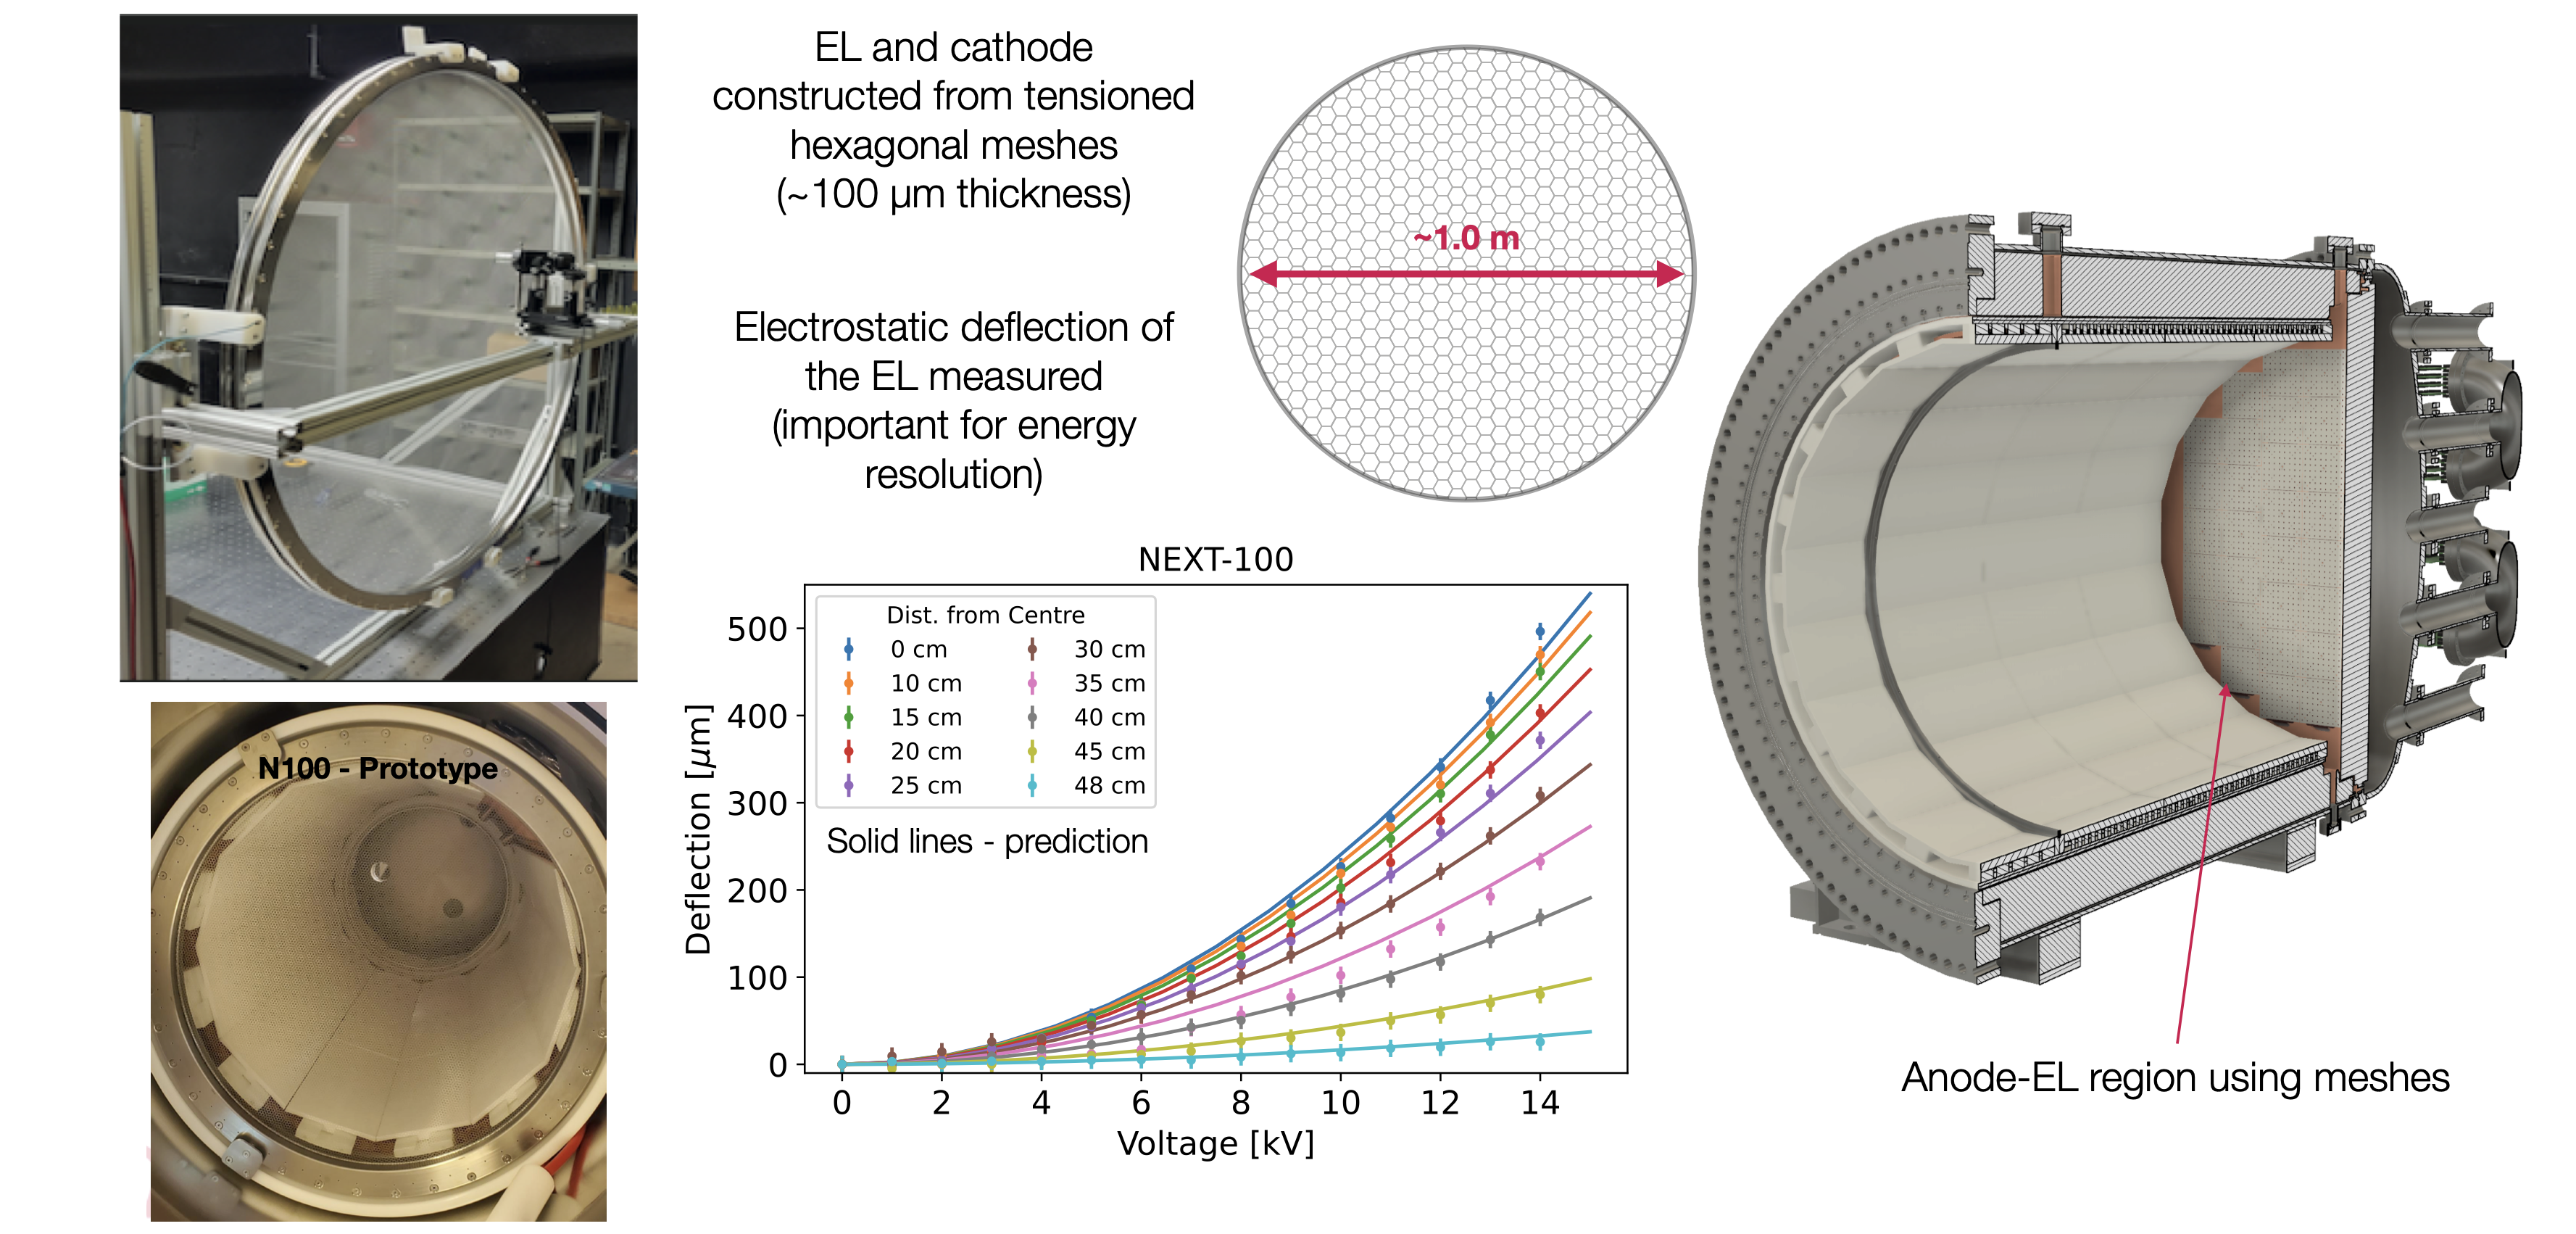
\includegraphics[scale=0.23]{meshes.png}

\end{frame}

%%

\begin{frame}{Cathode}

\includegraphics[scale=0.21]{cathodeMesh.png}

\end{frame}

%%

\begin{frame}{PMTs \& SiPMs}

\includegraphics[scale=0.23]{sipmandpmts.png}

\end{frame}

%%

\begin{frame}{Tracking Plane}

\includegraphics[scale=0.23]{trackingplaneNext100.png}

\end{frame}

\begin{frame}{Energy Plane}

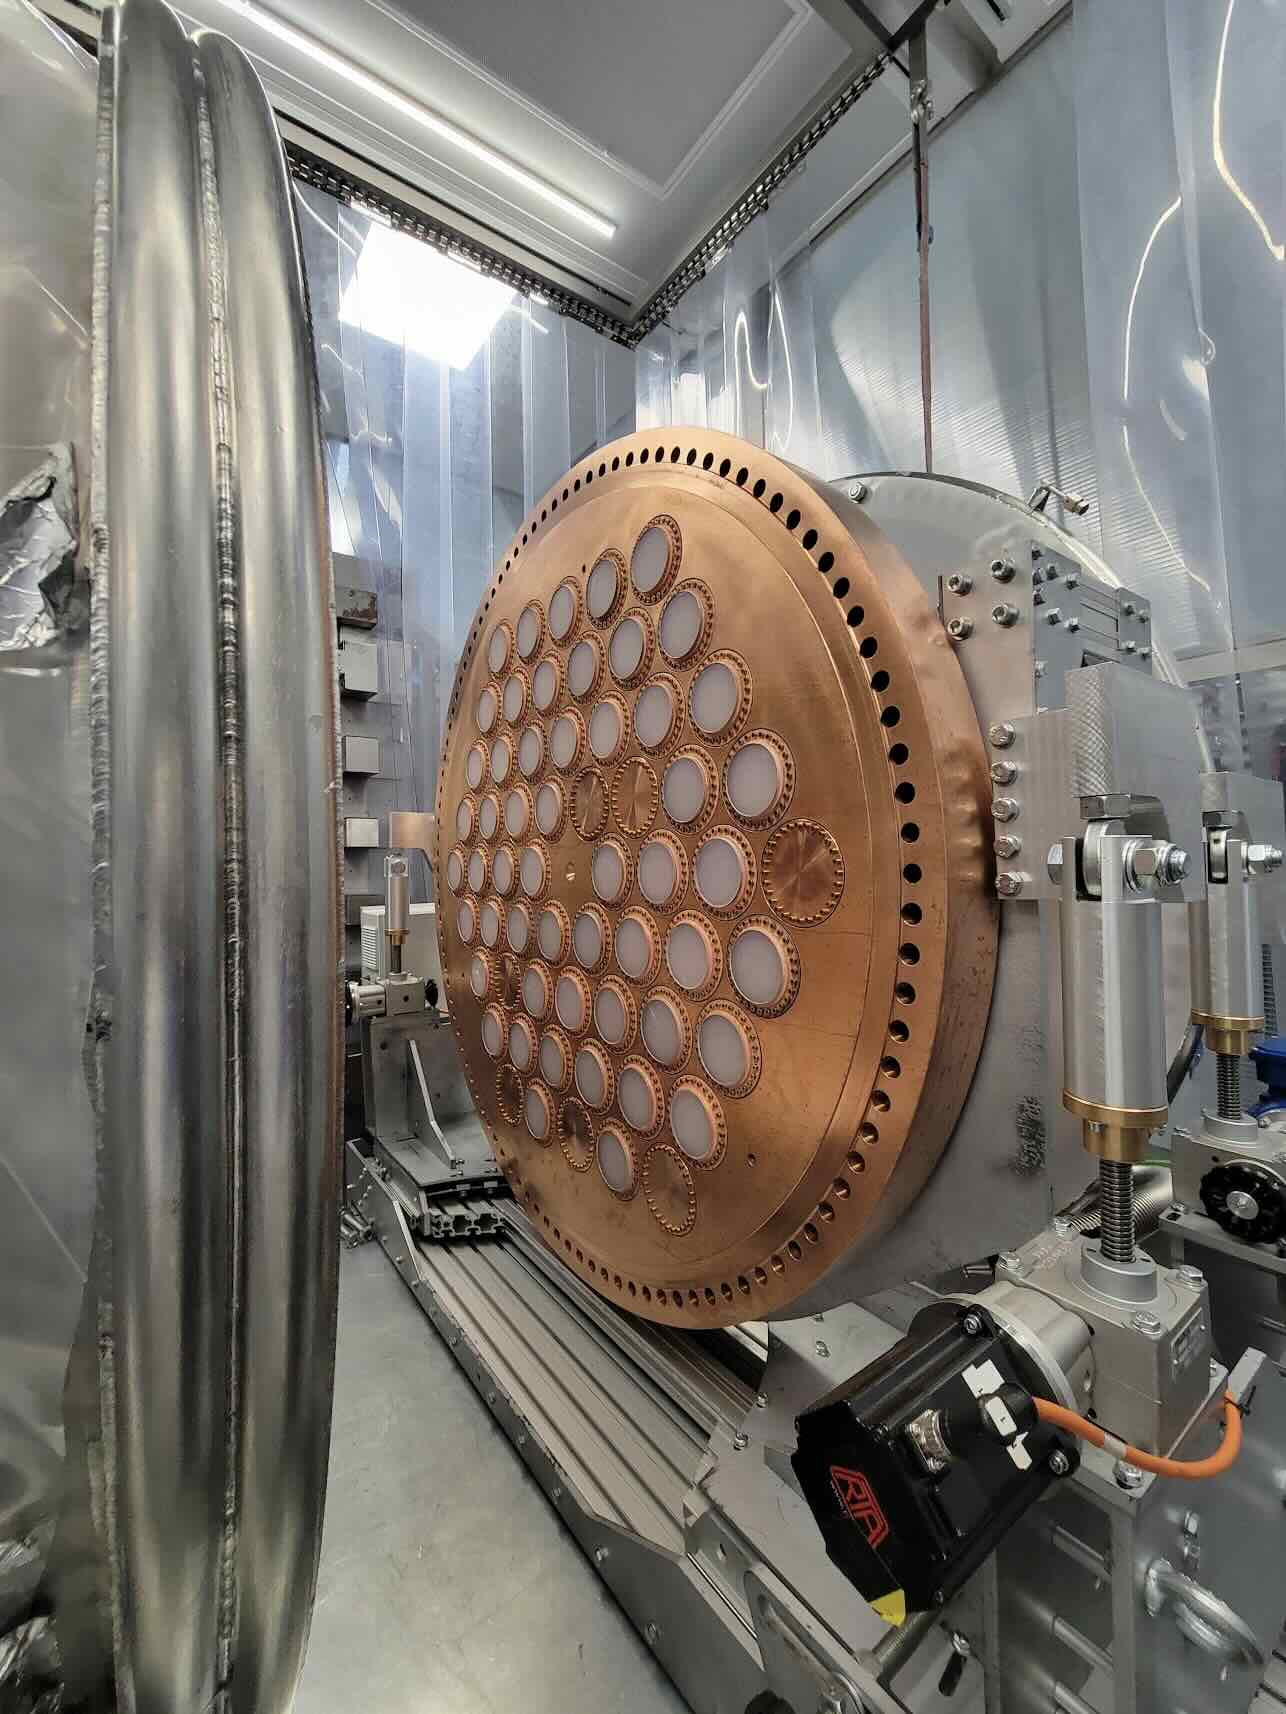
\includegraphics[scale=0.23]{n100-pmt.jpeg}

\end{frame}



%%%%%
\begin{frame}{Field Cage}

\includegraphics[scale=0.23]{fieldcage.png}

\end{frame}

%%%%%

\begin{frame}{Light Tube}

\includegraphics[scale=0.21]{LightTube.png}

\end{frame}

% \begin{frame}{The conceptual design}
%
%\begin{columns}
%\column{0.60\textwidth}
%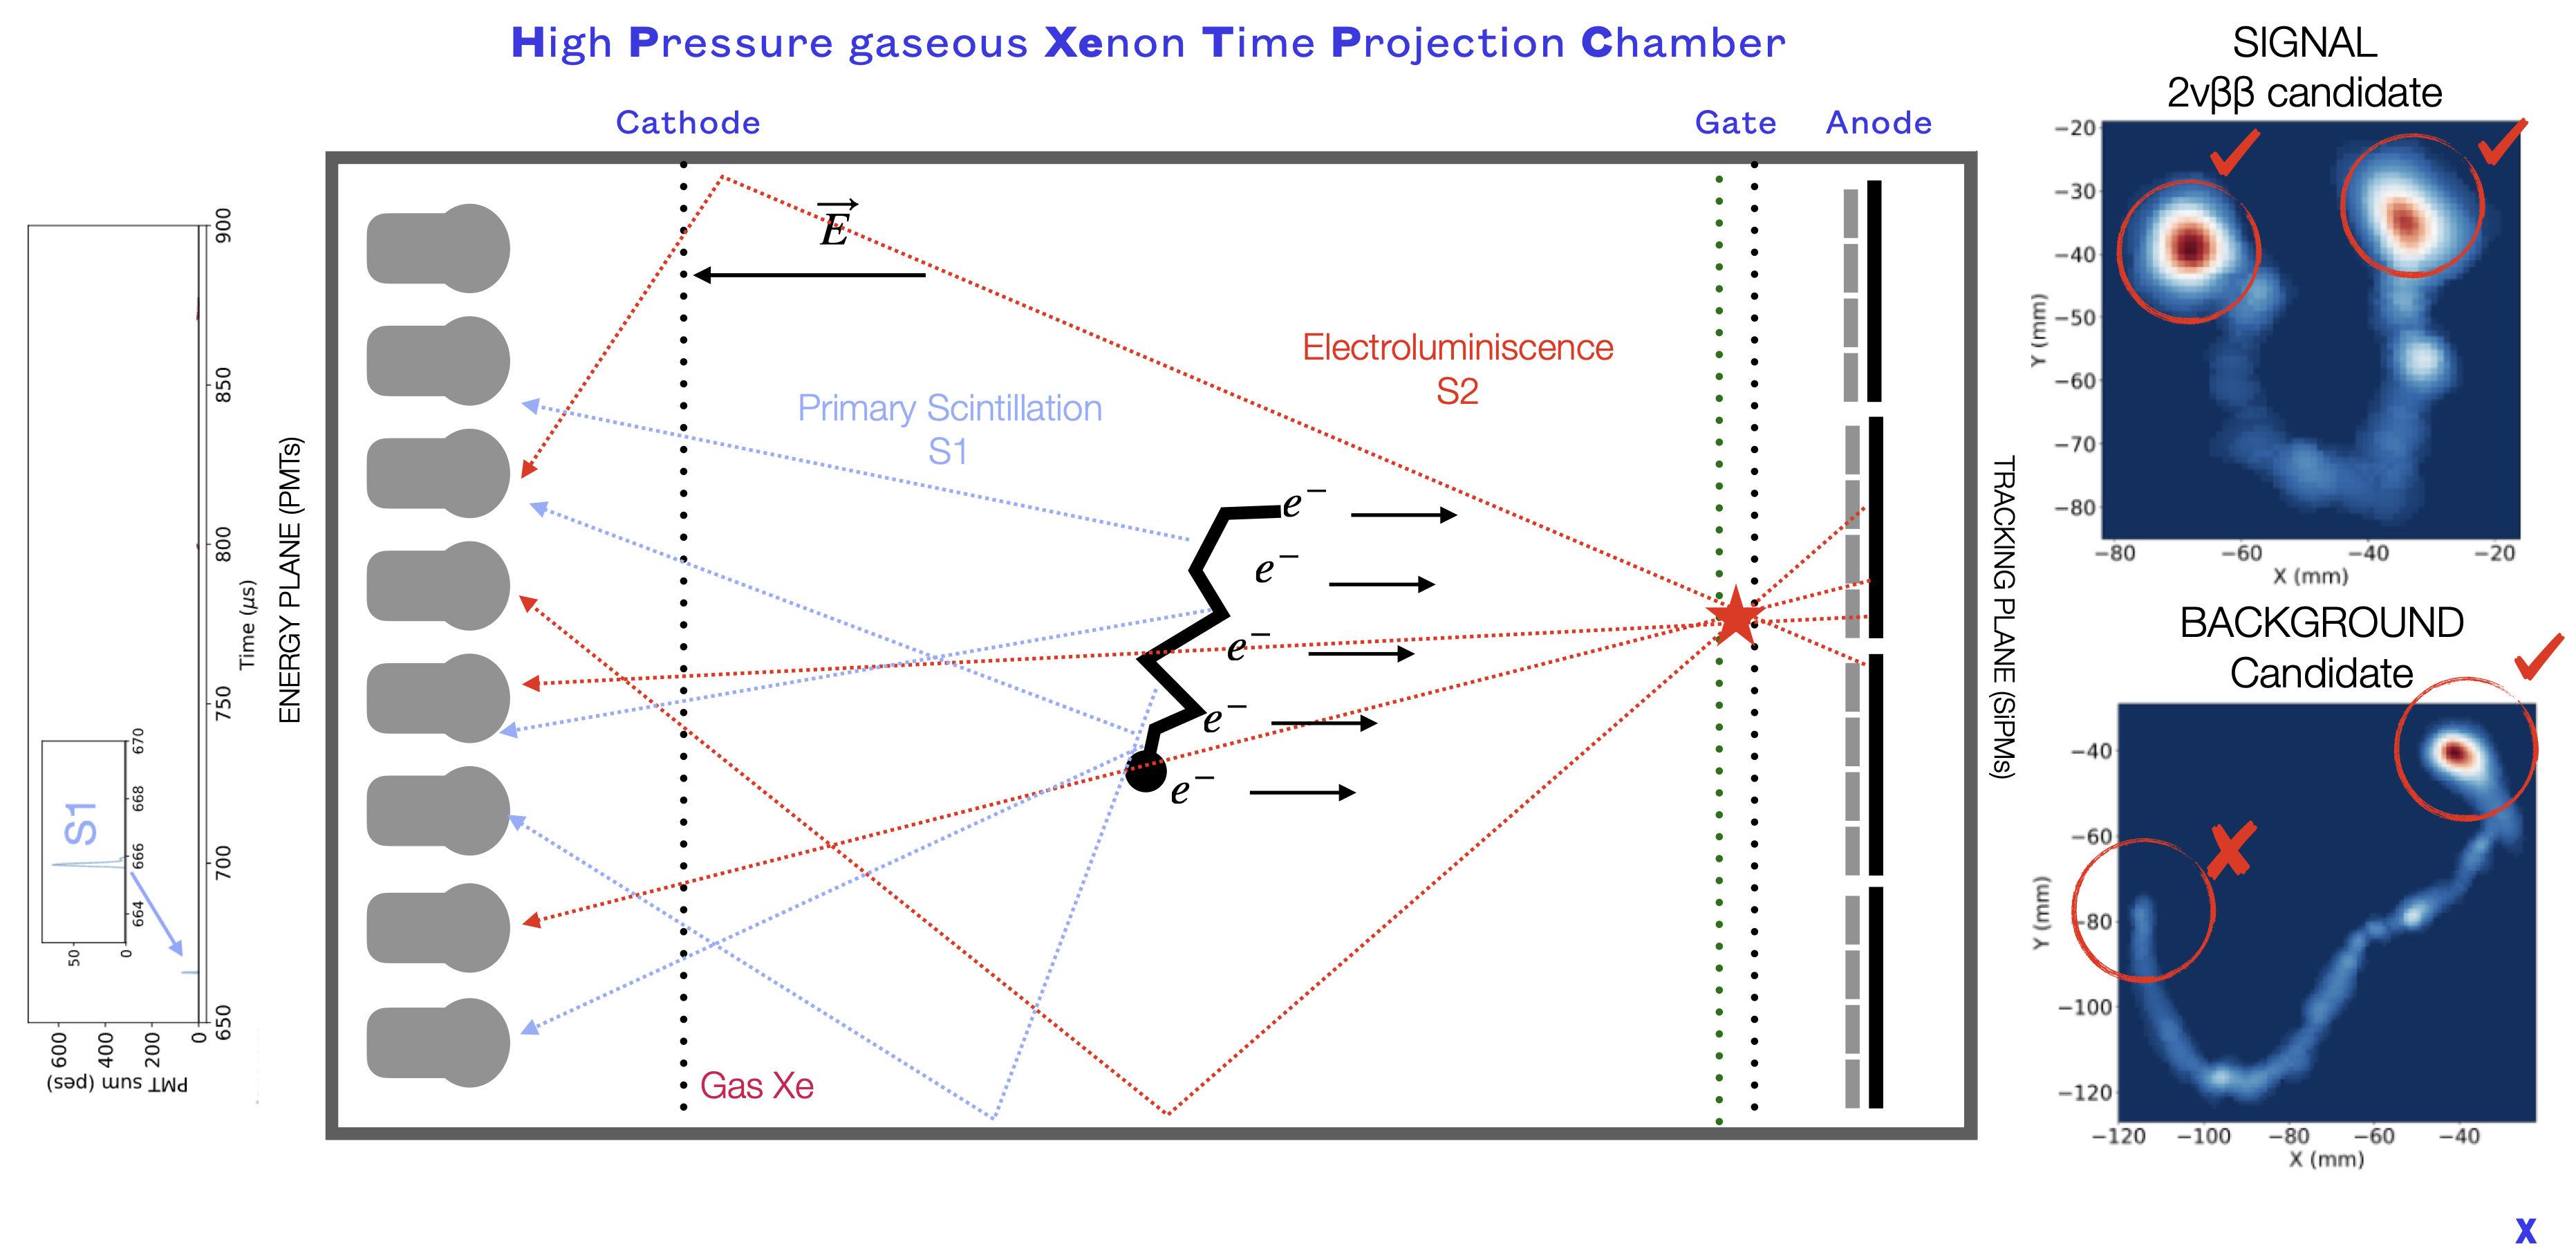
\includegraphics[scale=0.14]{nexttraum.png}
%
%
% \column{0.40\textwidth}
%$\bullet~$ NEXT  was originally conceived as a EL TPC  with an energy plane (PMTs to integrate as much as the emitted signal as possible) and a tracking plane (made os SiPMs in order to pixelise the track) was born.  
%
%$\bullet~$ The working pressure could be anything between 5-20 bar. High pressure allows more mass per unit volume, but implies higher electric fields and more diffusion, thus, potentially weakening the topological signature. 
%
%\end{columns}
%\end{frame}

\begin{frame}{Energy resolution in NEXT}

\begin{columns}
\column{0.50\textwidth}
$\bullet~$ NEXT-White

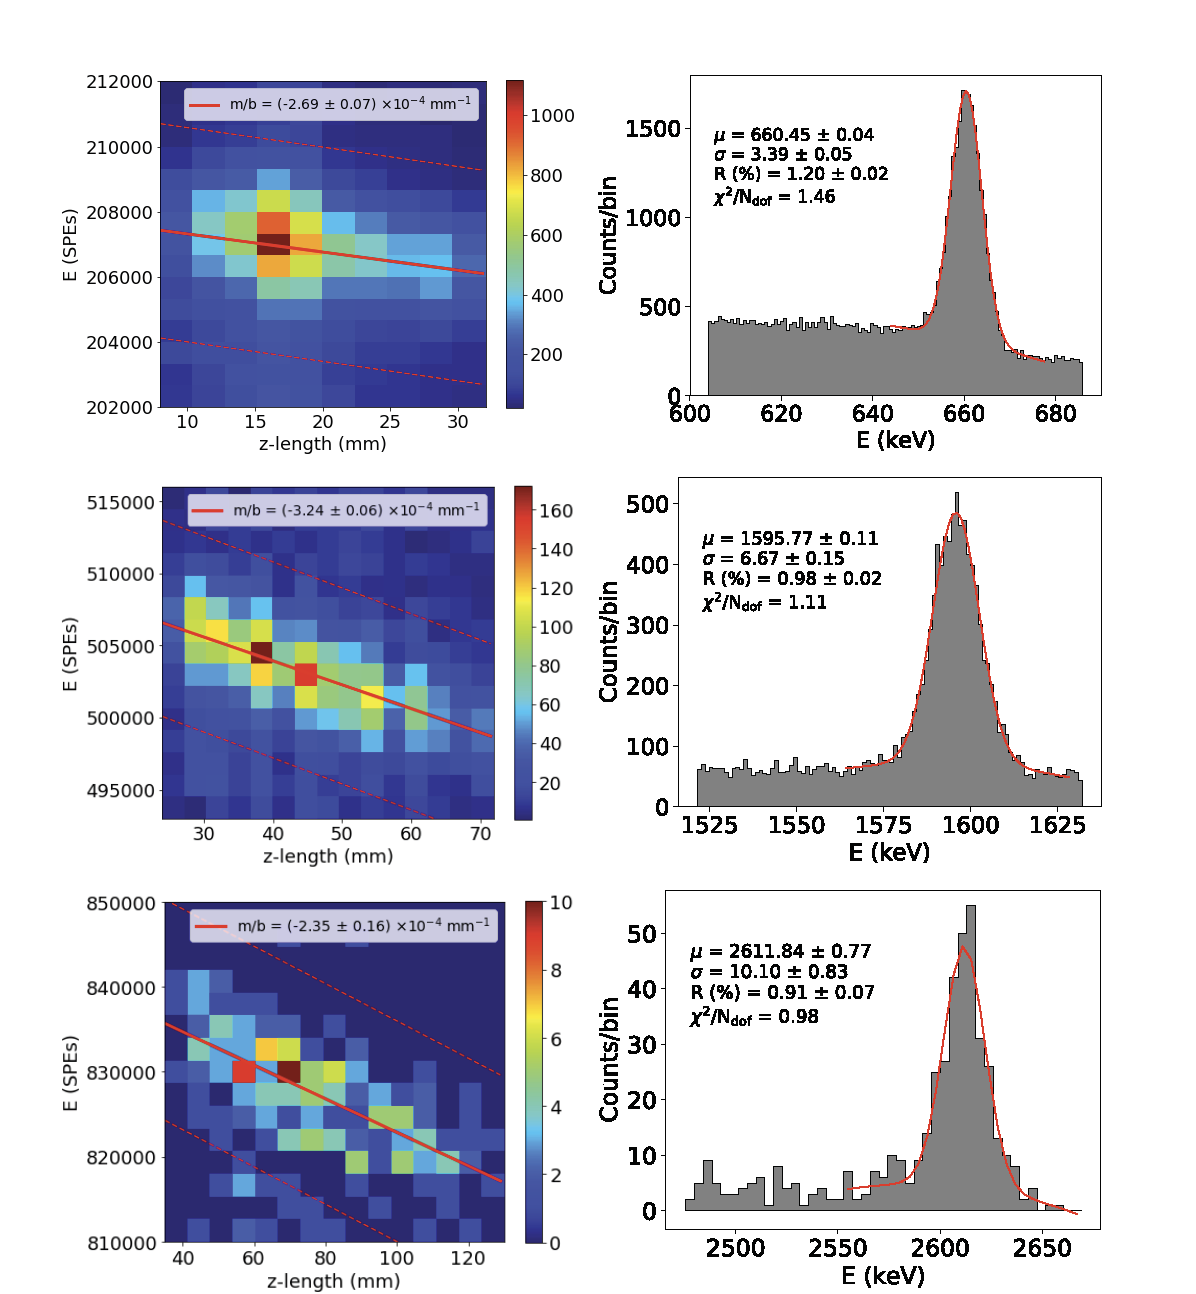
\includegraphics[scale=0.21]{eresWhite.png}

 \column{0.50\textwidth}
 $\bullet~$ NEXT-100 (Krypton) 
 
 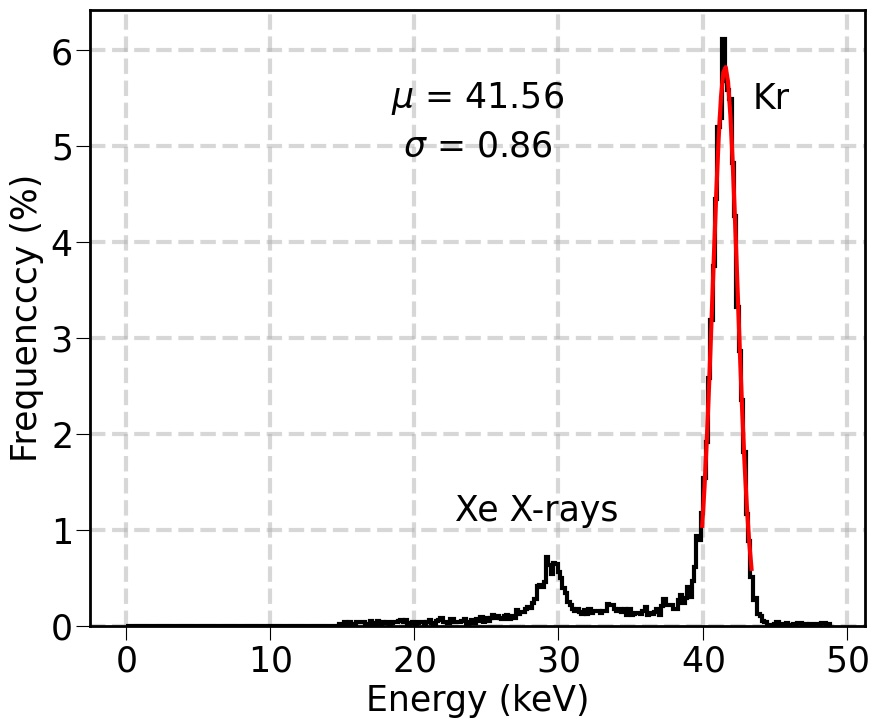
\includegraphics[scale=0.23]{kr_energy_fiducial.jpeg}
 
%$\bullet~$ NEXT-White measured an energy resolution of $\sim 0.9$\% at \qbb.
%
%$\bullet~$ This is a good result, but not as good as the one obtained with DBDM or expected from basic principles. 
%
%$\bullet~$ Possible effects entering the resolution: a) residuals in geometry correction (fix: a more homogenous ``energy plane''); b) residual associated to the lifetime, which in NEXT-White was of the order of several ms (fix: longer lifetime); c) residual associated to track length (fix: shorter tracks?) 
  
\end{columns}
\end{frame}

\begin{frame}{Topological signature}
\begin{columns}
\column{0.60\textwidth}
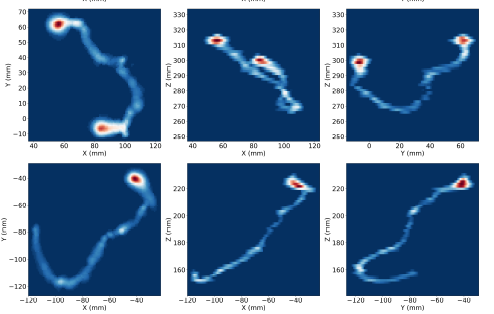
\includegraphics[scale=0.50]{deconv1e2e.png}
 \column{0.40\textwidth}

$\bullet~$ Real data electrons and double electrons from the 1.6 MeV double escape peak of \TL) 
 \end{columns}
\end{frame}

%\begin{frame}{Applying the topological signature}
%\begin{columns}
%\column{0.60\textwidth}
%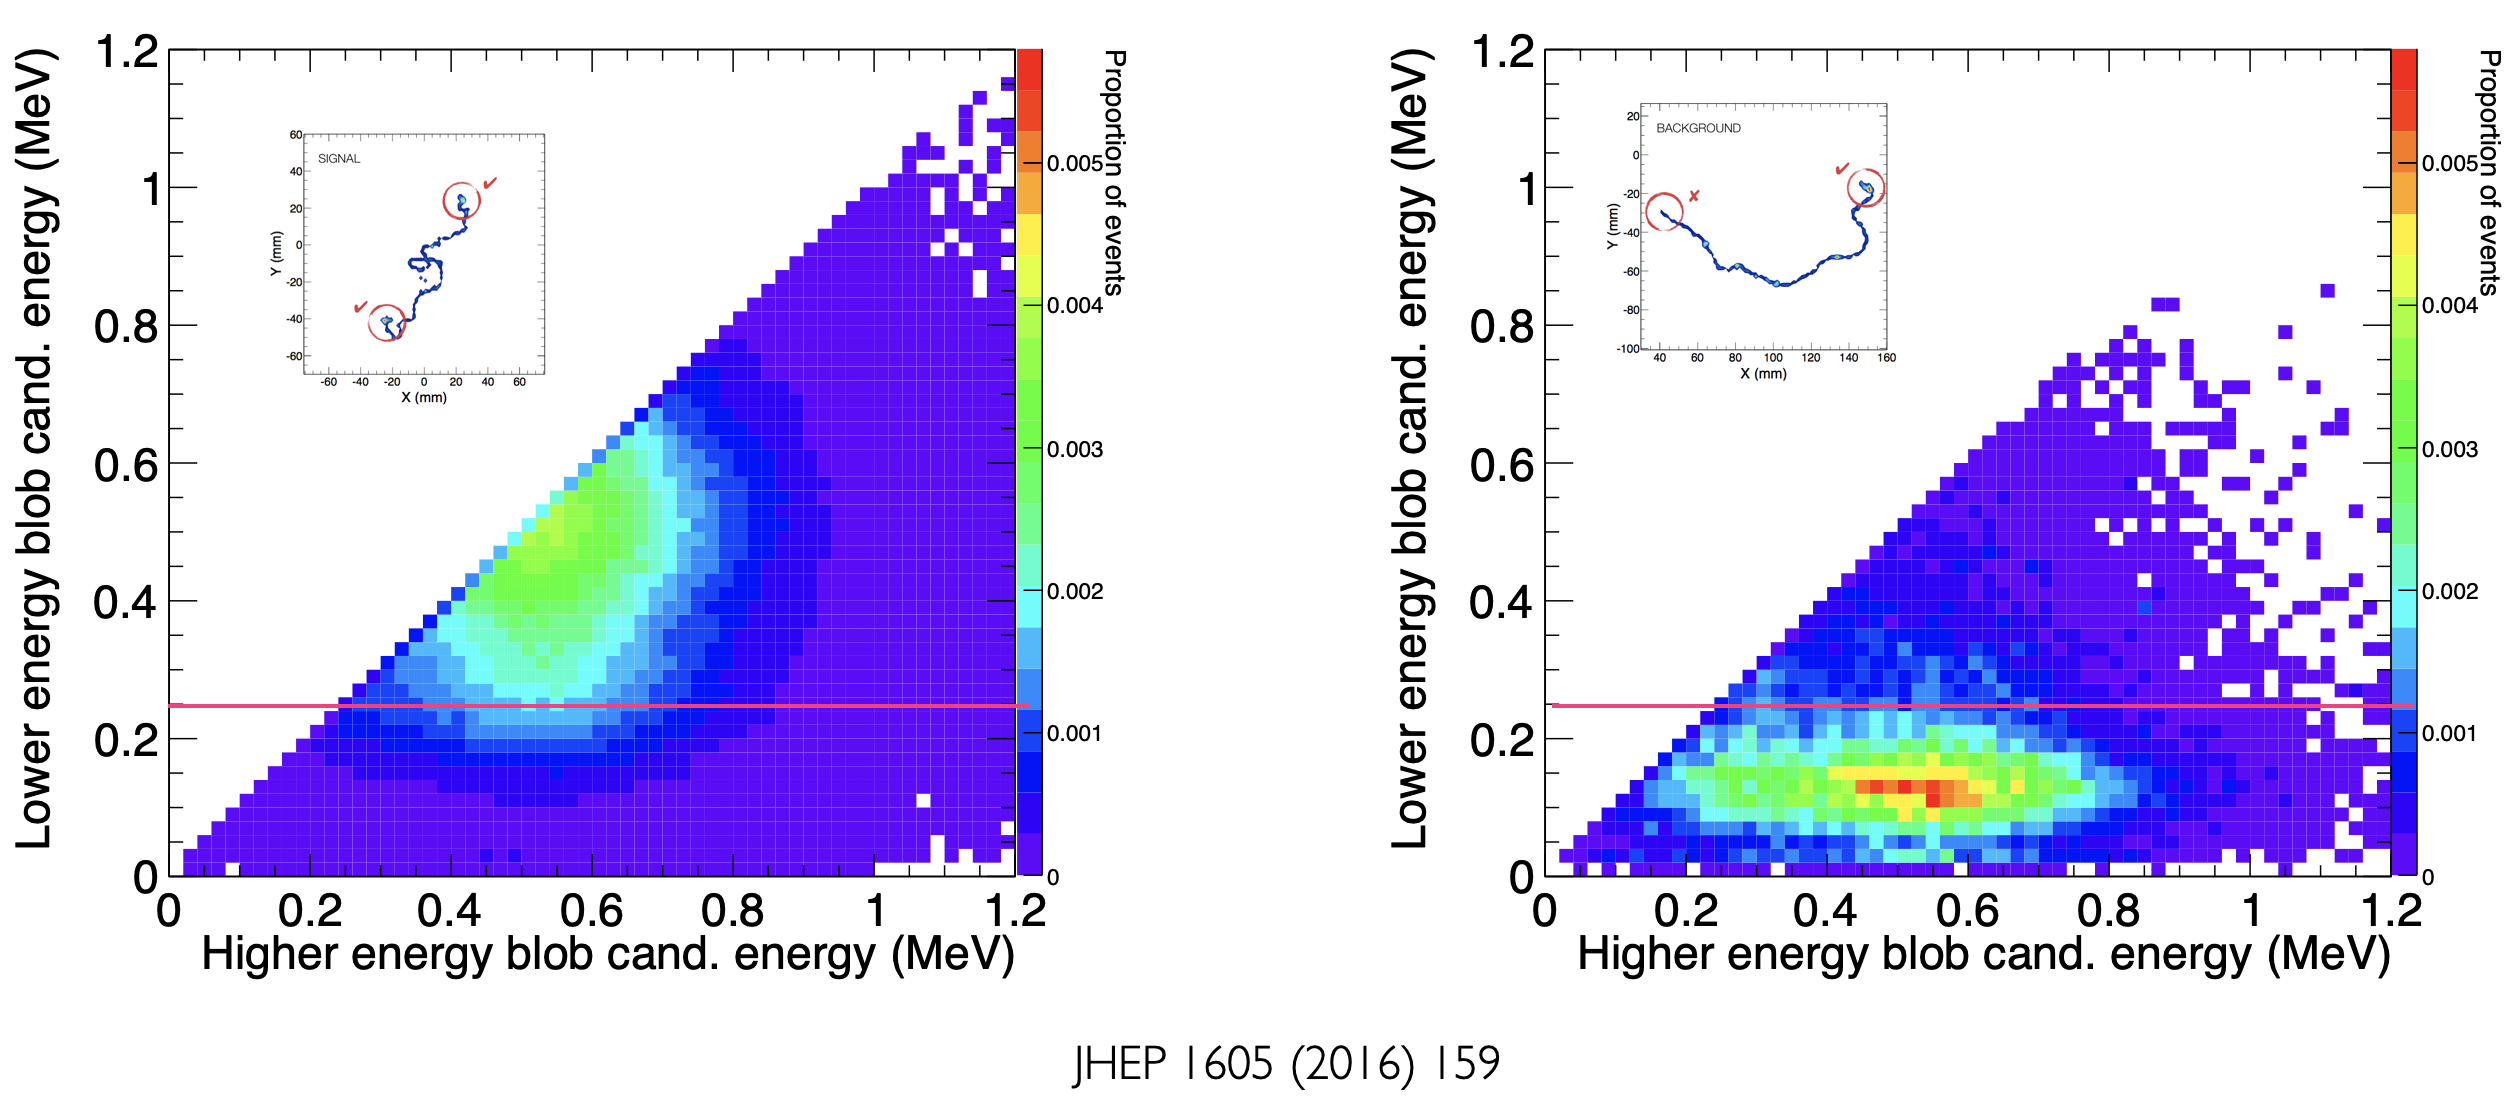
\includegraphics[scale=0.30]{topoNew.png}
 %\column{0.40\textwidth}

%$\bullet~$ After deconvolution, we can recover a clean topological signature (1e vs 2e), in spite of diffusion (these are real data electrons and double electrons from the 1.6 MeV double escape peak of \TL) 
 %\end{columns}
%\end{frame}

\begin{frame}{Energy Spectrum}
\begin{columns}
\column{0.60\textwidth}
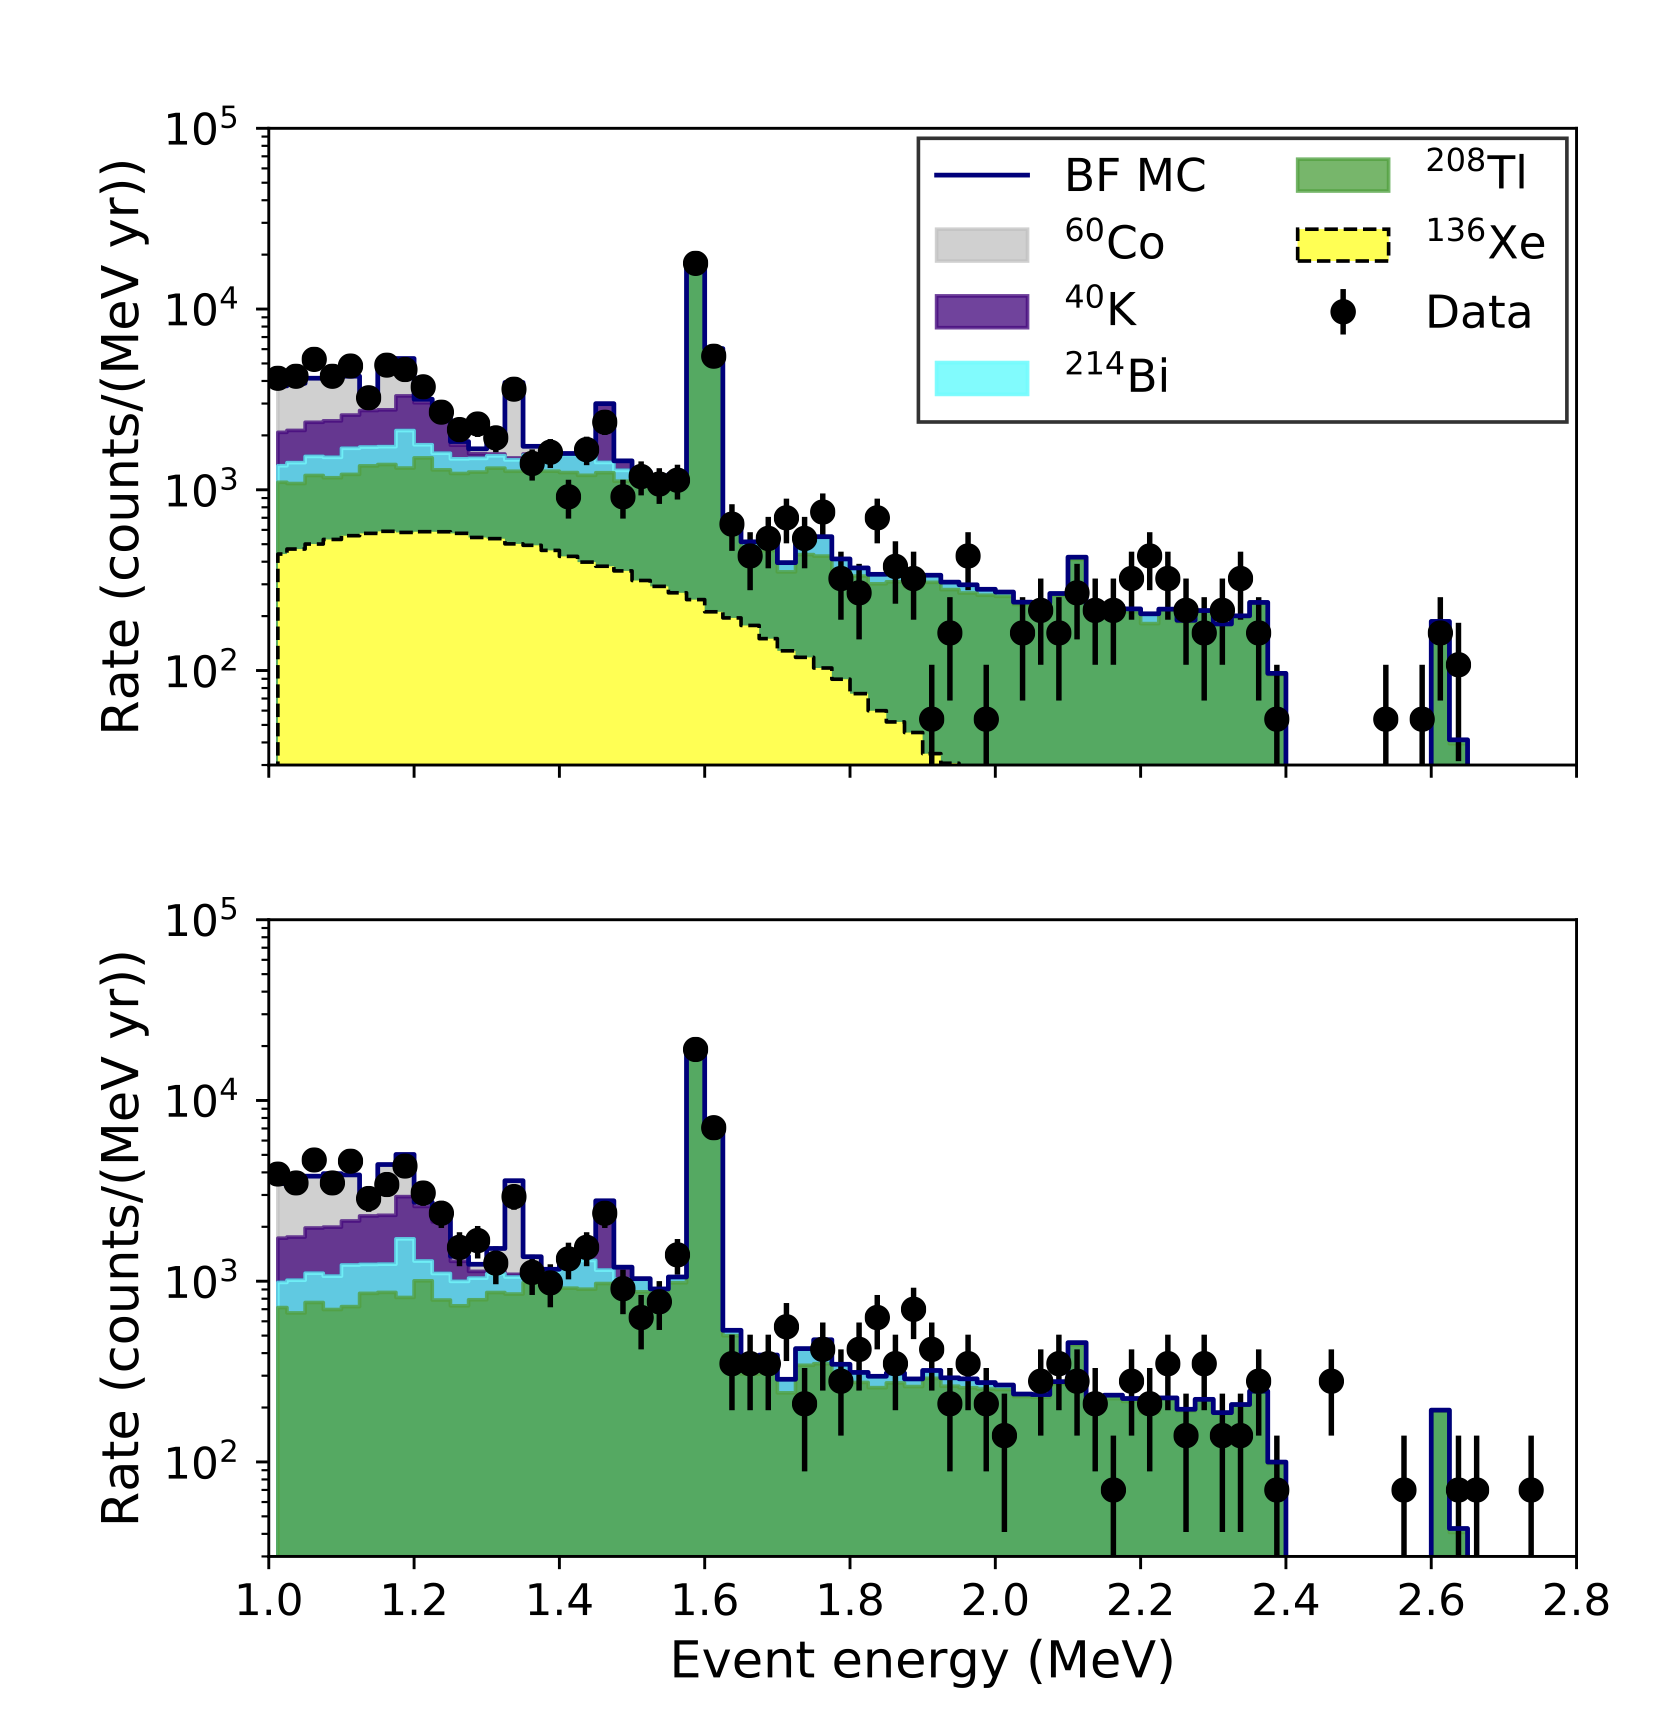
\includegraphics[scale=0.26]{newSpectrum.png}
\column{0.40\textwidth}

$\bullet~$ Energy spectrum measured by NEXT-White. A Xenon TPC like NEXT can run with depleted xenon (no \XE) and with enriched xenon (90\% of \XE) and compared results, thus reducing very much the dependence with the Monte Carlo. 

$\bullet~$ Notice the hole around \qbb, where a putative signal may show up. 
 \end{columns}
\end{frame}

%\begin{frame}{\bbtnu\ mode}
%\begin{columns}
%\column{0.60\textwidth}
%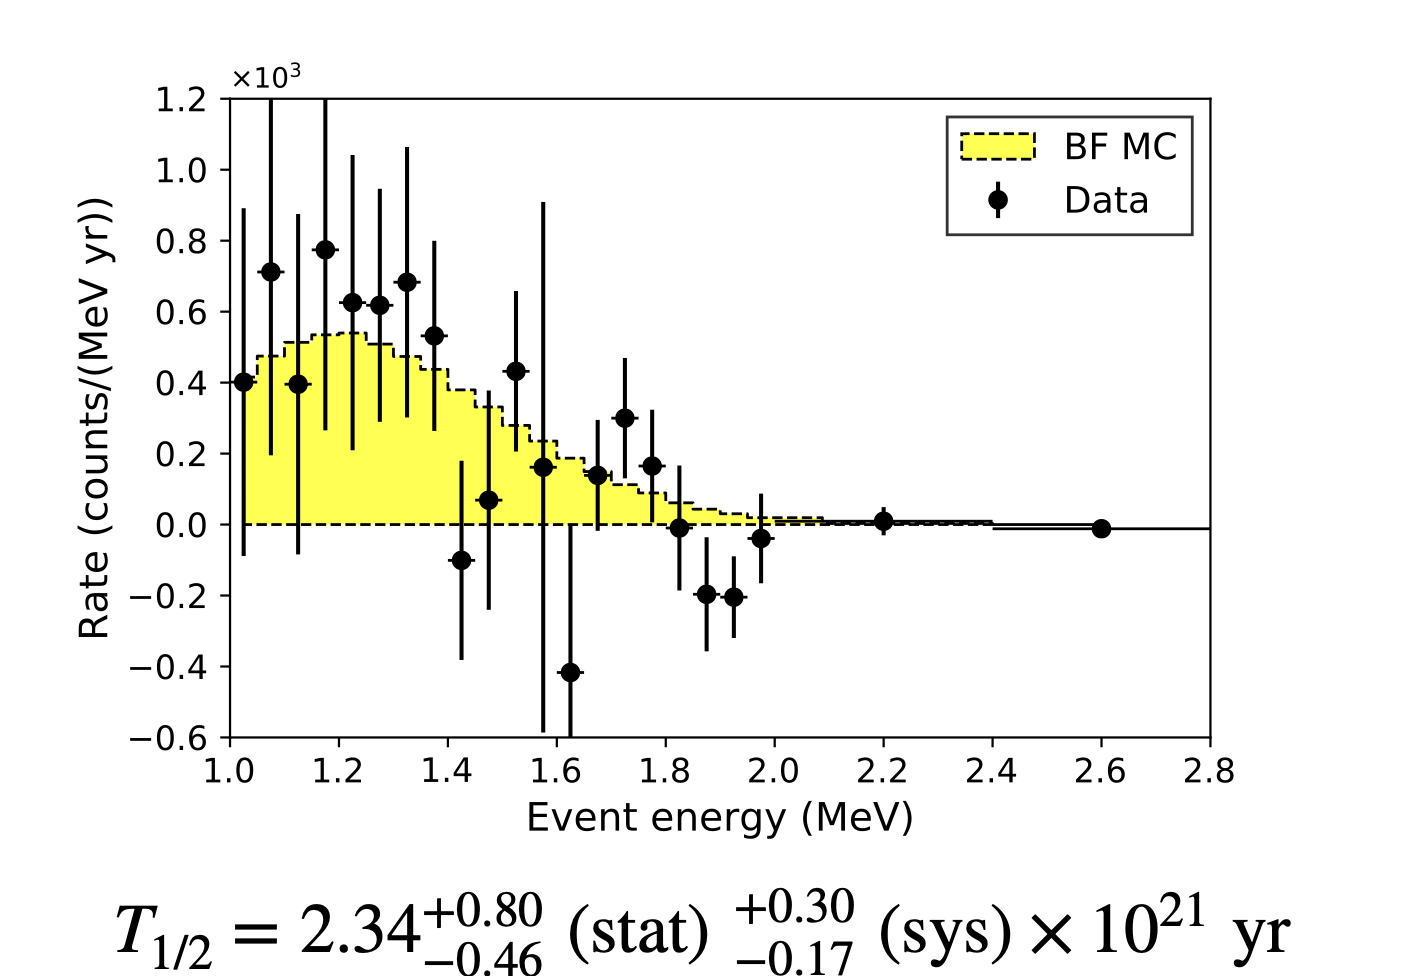
\includegraphics[scale=0.36]{bb2nu.png}
%\column{0.40\textwidth}
%
%$\bullet~$ Although NEXT-White is a relatively small detector (5 kg of active volume), it has been able to measure the \bbtnu\ mode (St. Gotthard TPC, with a similar mass couldn't do it, due to backgrounds). 
%
%$\bullet~$ In particular, in NEXT-White has been possible to measure the \bbtnu\ mode using direct subtraction between the data with enriched and depleted xenon. 
% \end{columns}
%\end{frame}

%%%

\begin{frame}{Status of NEXT-100/N100U}

$\bullet$ Begin operations at 5 bar (low pressure run) in 2024.

$\bullet$ LPR will carry on until summer 2025, with the goal of measuring detector performance (energy resolution, topological signature, calibrations).


$\bullet$ High pressure run (13 bar) in starts in summer 2025 and extends until early 2028, with the goal of measuring backgrounds, perform a high statistical measurement of the \bbtnu\ signal and perform a search for \bbonu\ events. 

$\bullet$ Upgrade in the first half of 2028 (NEXT-100 becomes N100U). 

$\bullet$ N100U operates until 2030 (reduced background budget, enhanced sensitivity).

\end{frame}

\begin{frame}{The NEXT program (first 20 years)}

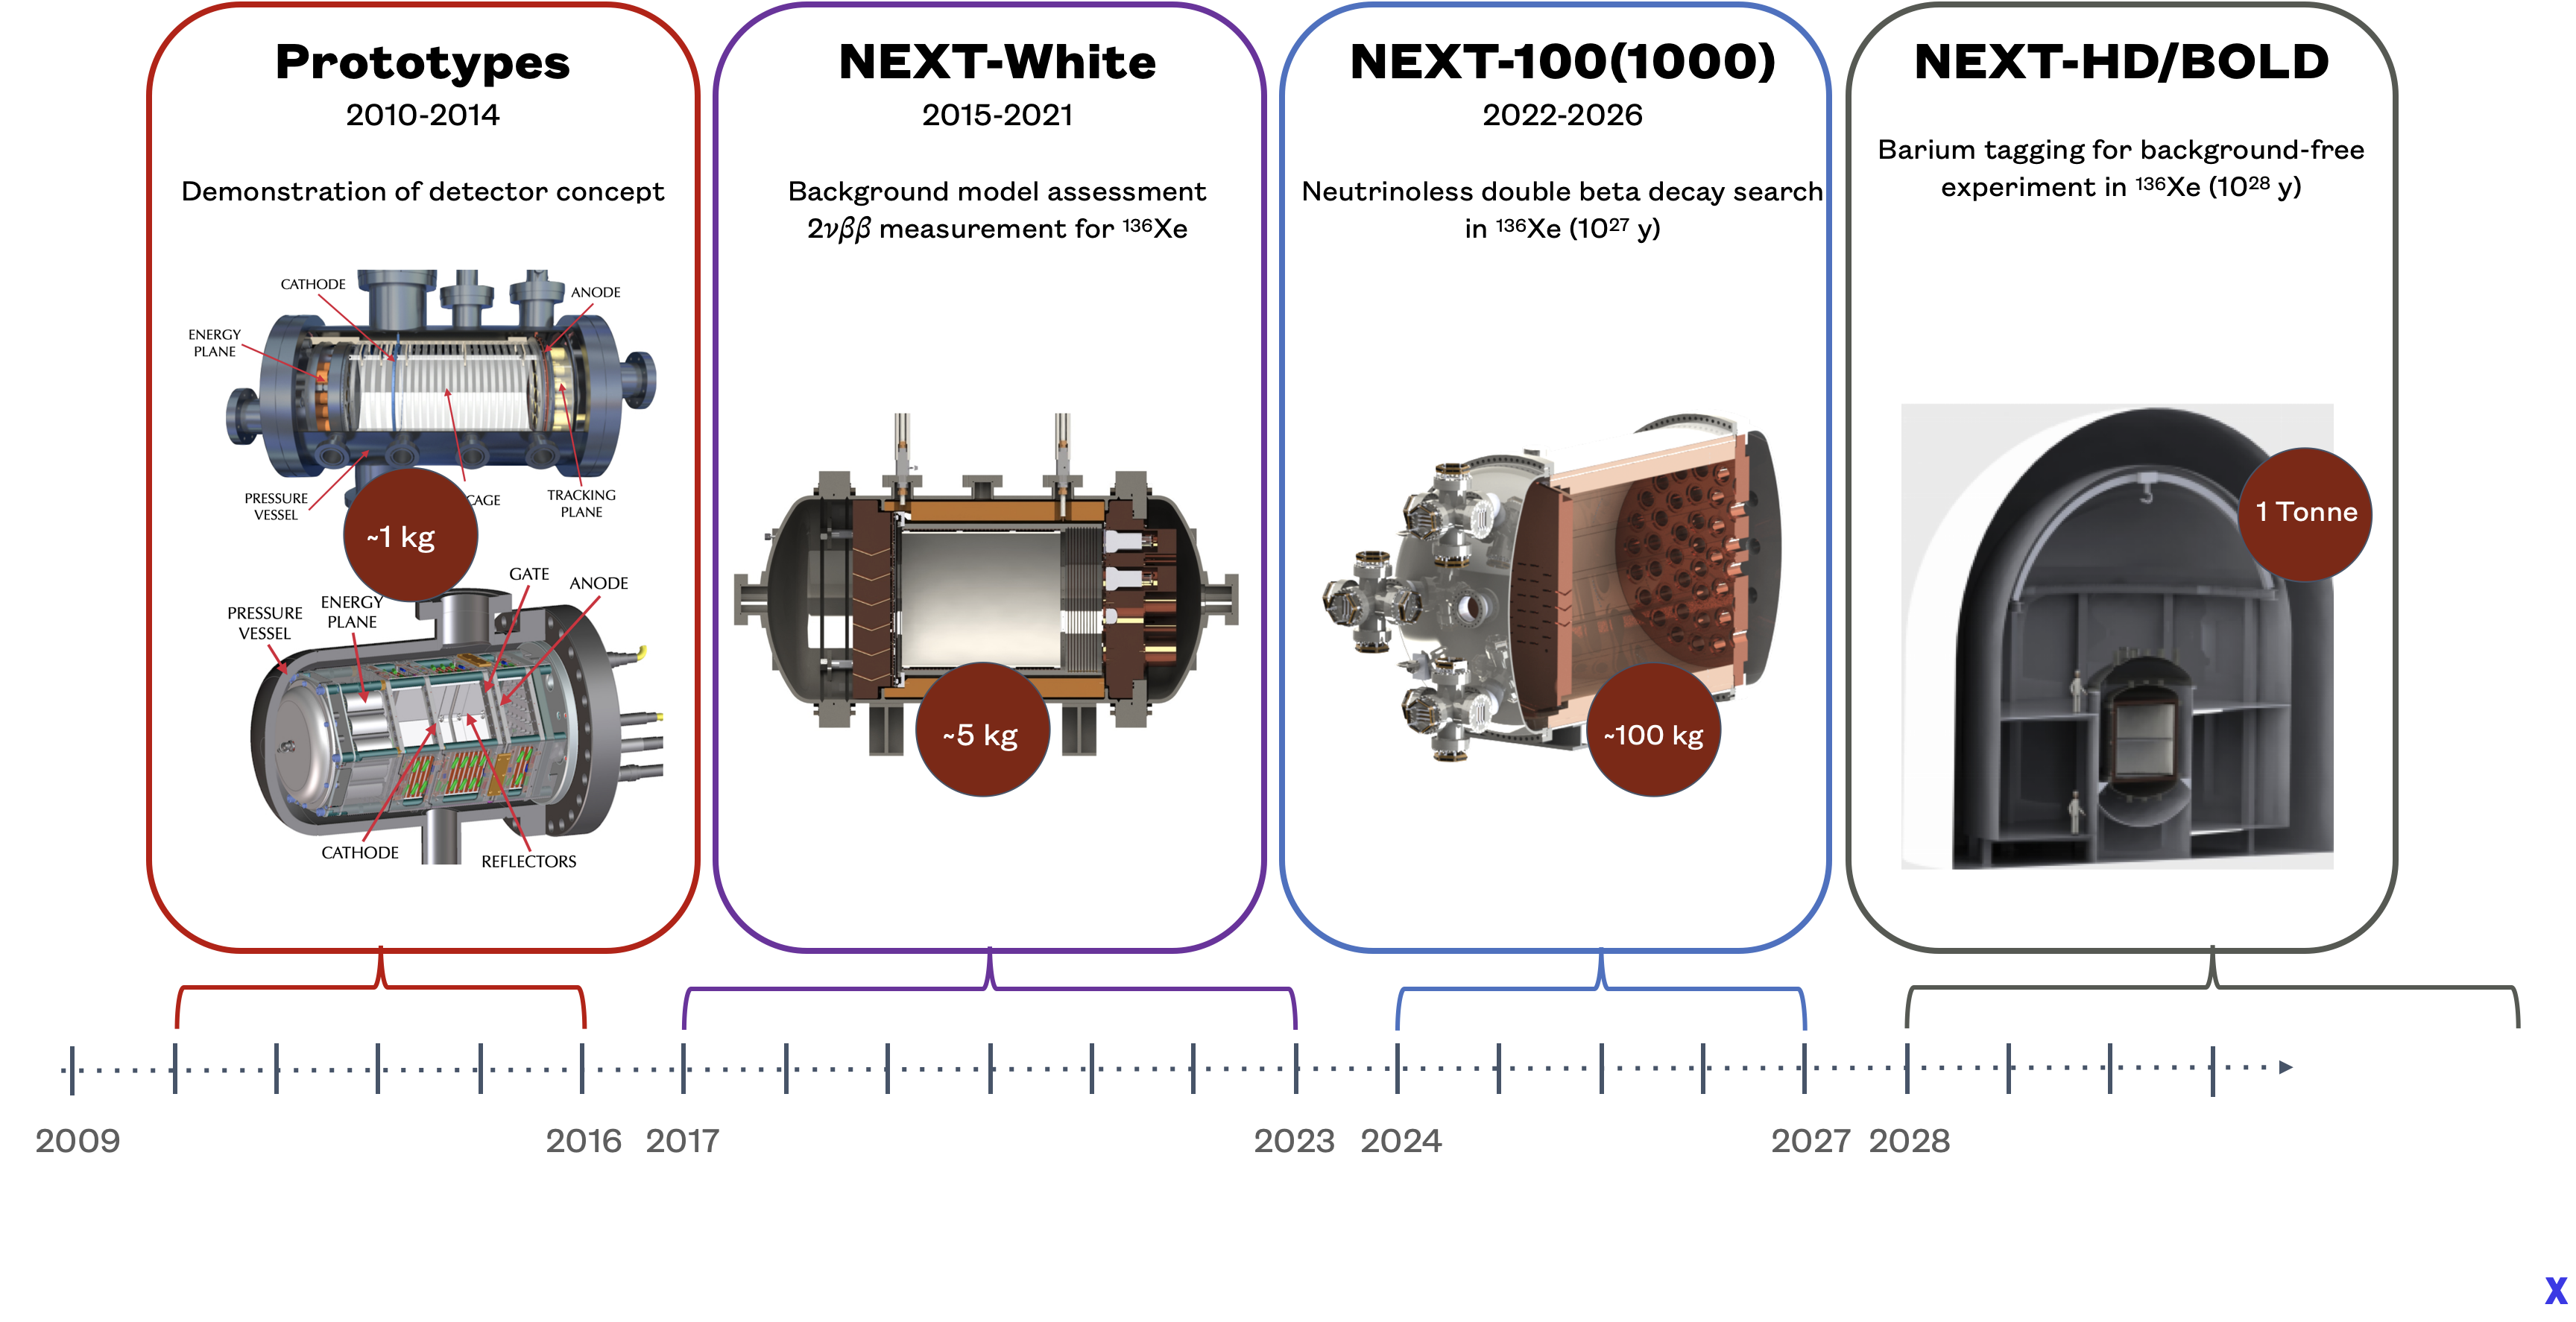
\includegraphics[scale=0.23]{nextprogram.png}

\end{frame}

\begin{frame}{N100U}
\begin{columns}
\column{0.60\textwidth}
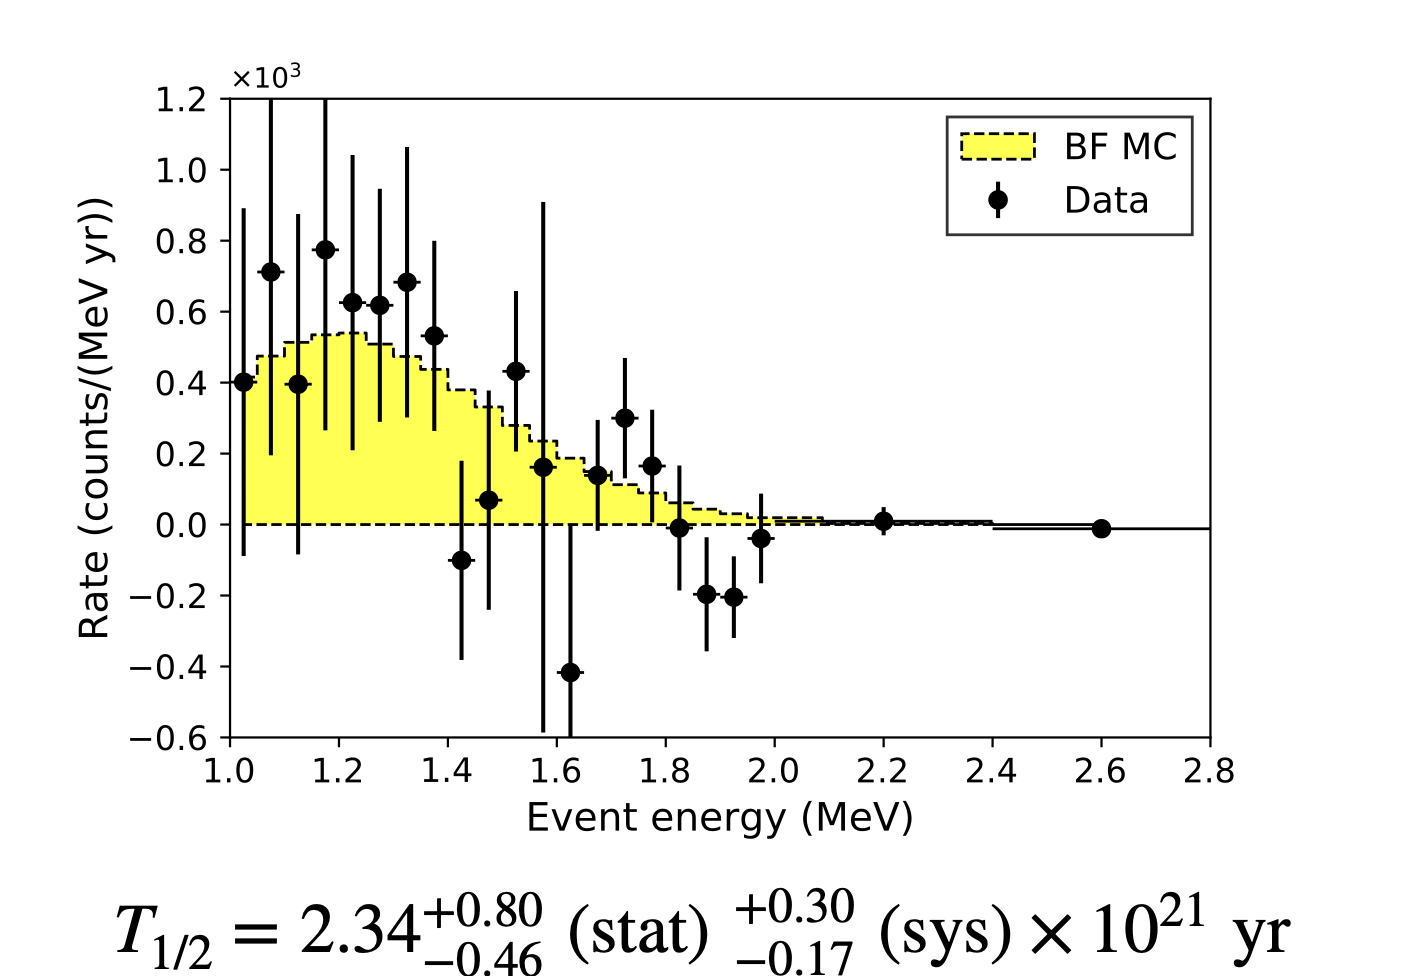
\includegraphics[scale=0.36]{bb2nu.png}
\column{0.40\textwidth}
\end{columns}
\end{frame}



%%\begin{frame}{Sailing to Ithaca}
%%\begin{colum
%%%%


\begin{frame}{NEXT-HD}
\begin{columns}
\column{0.50\textwidth}
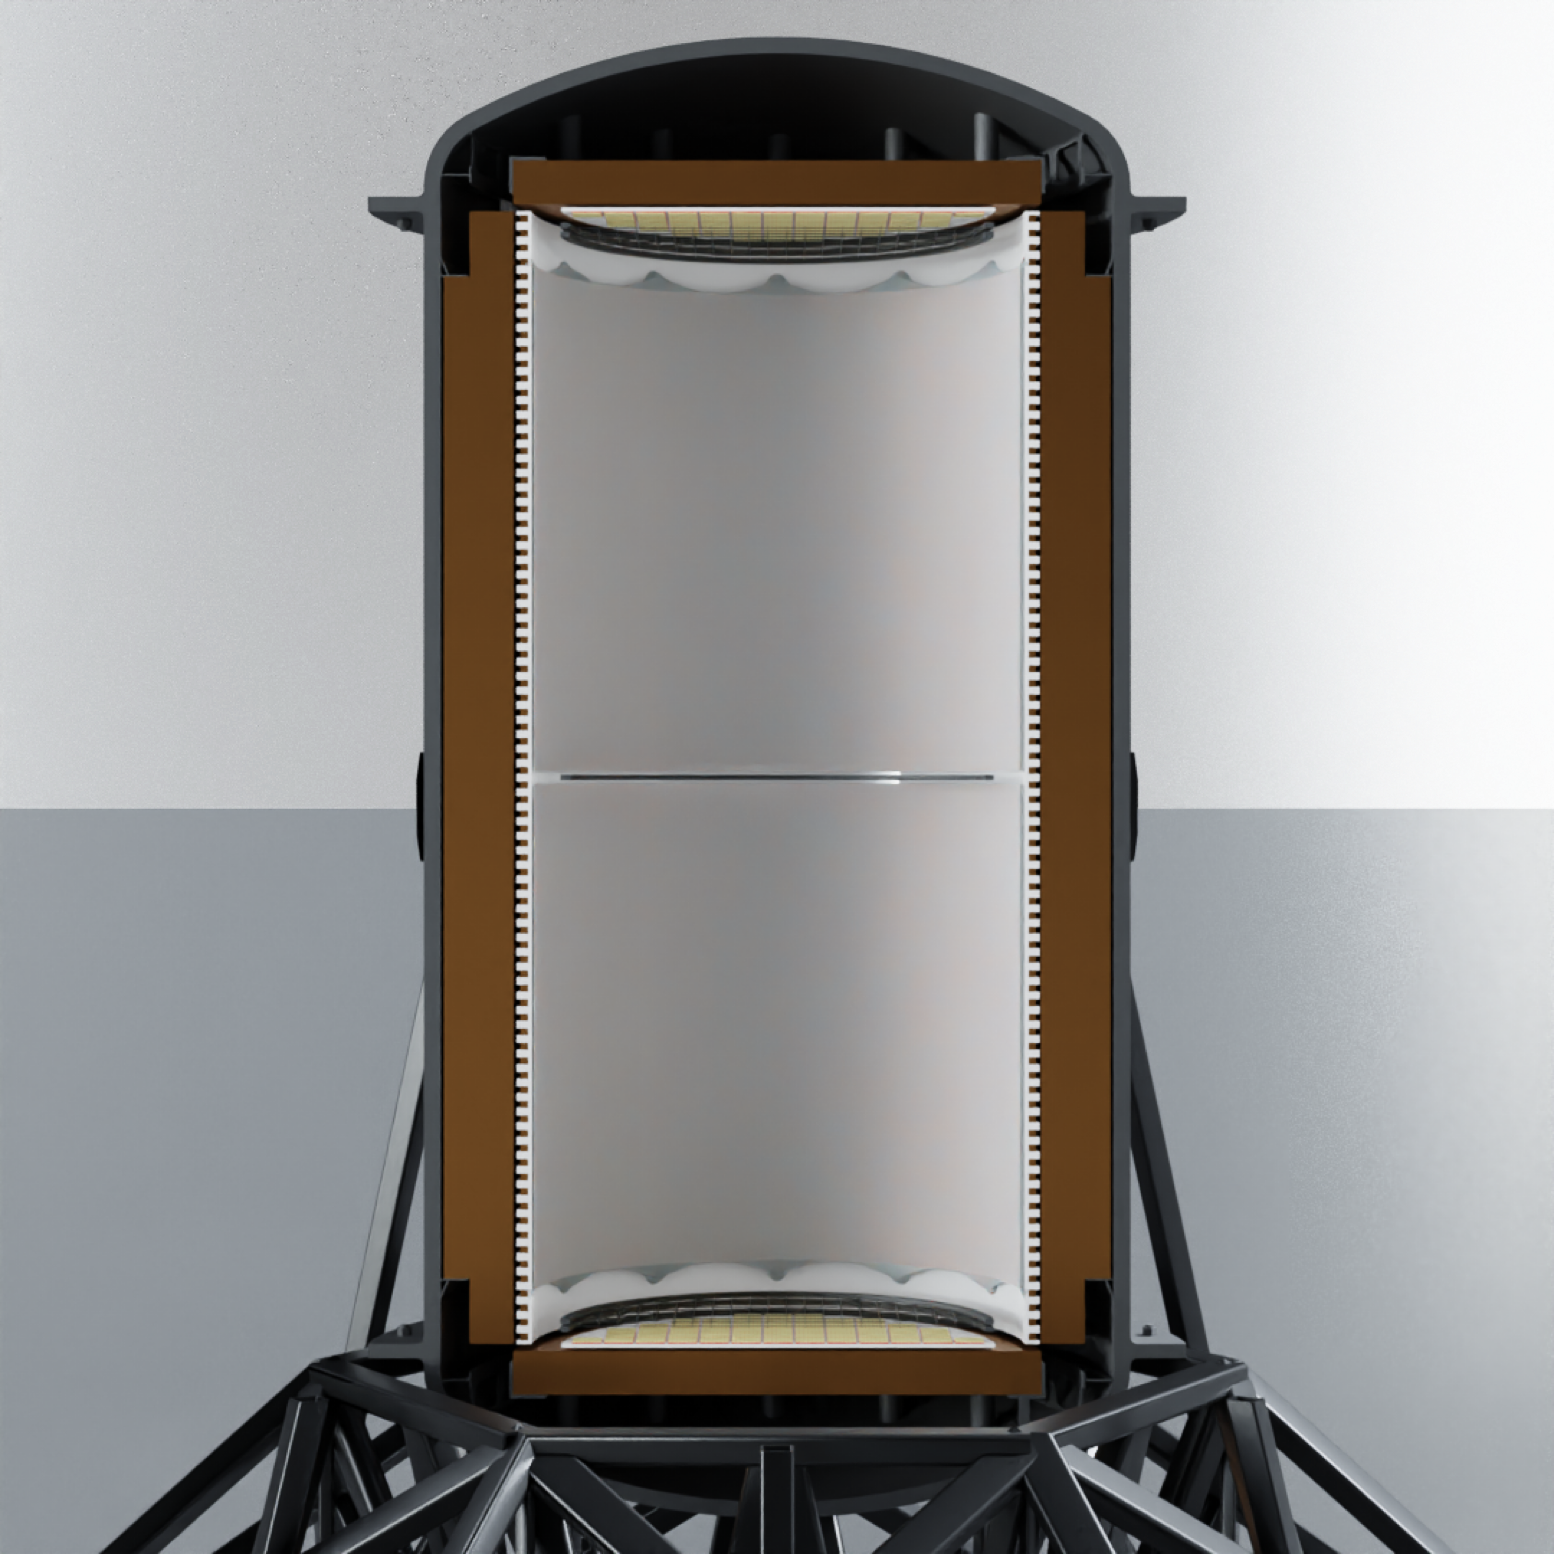
\includegraphics[scale=0.28]{nextHD.png}

\column{0.50\textwidth}

$\bullet~$ {\bf Scale up dimensions}: A symmetric detector of $2 \times 1.5$~m length and $2.2$~m diameter, ``doubling size of NEXT-100'',  holds 1 tonne at 15 bar and allows operational voltages in the same range than those used by NEXT-100 (thus, minimising risk).

$\bullet~$ {\bf Eliminate PMTs}, which introduce a substantial background and are difficult to operate at high pressure (also, PMTs do not allow a symmetric detector). 

$\bullet~$ {\bf Vertical orientation} simplifies mechanics. 

\end{columns}
\end{frame}
  
%  \begin{frame}{Barrel Fiber Detector}
%\begin{columns}
%\column{0.50\textwidth}
%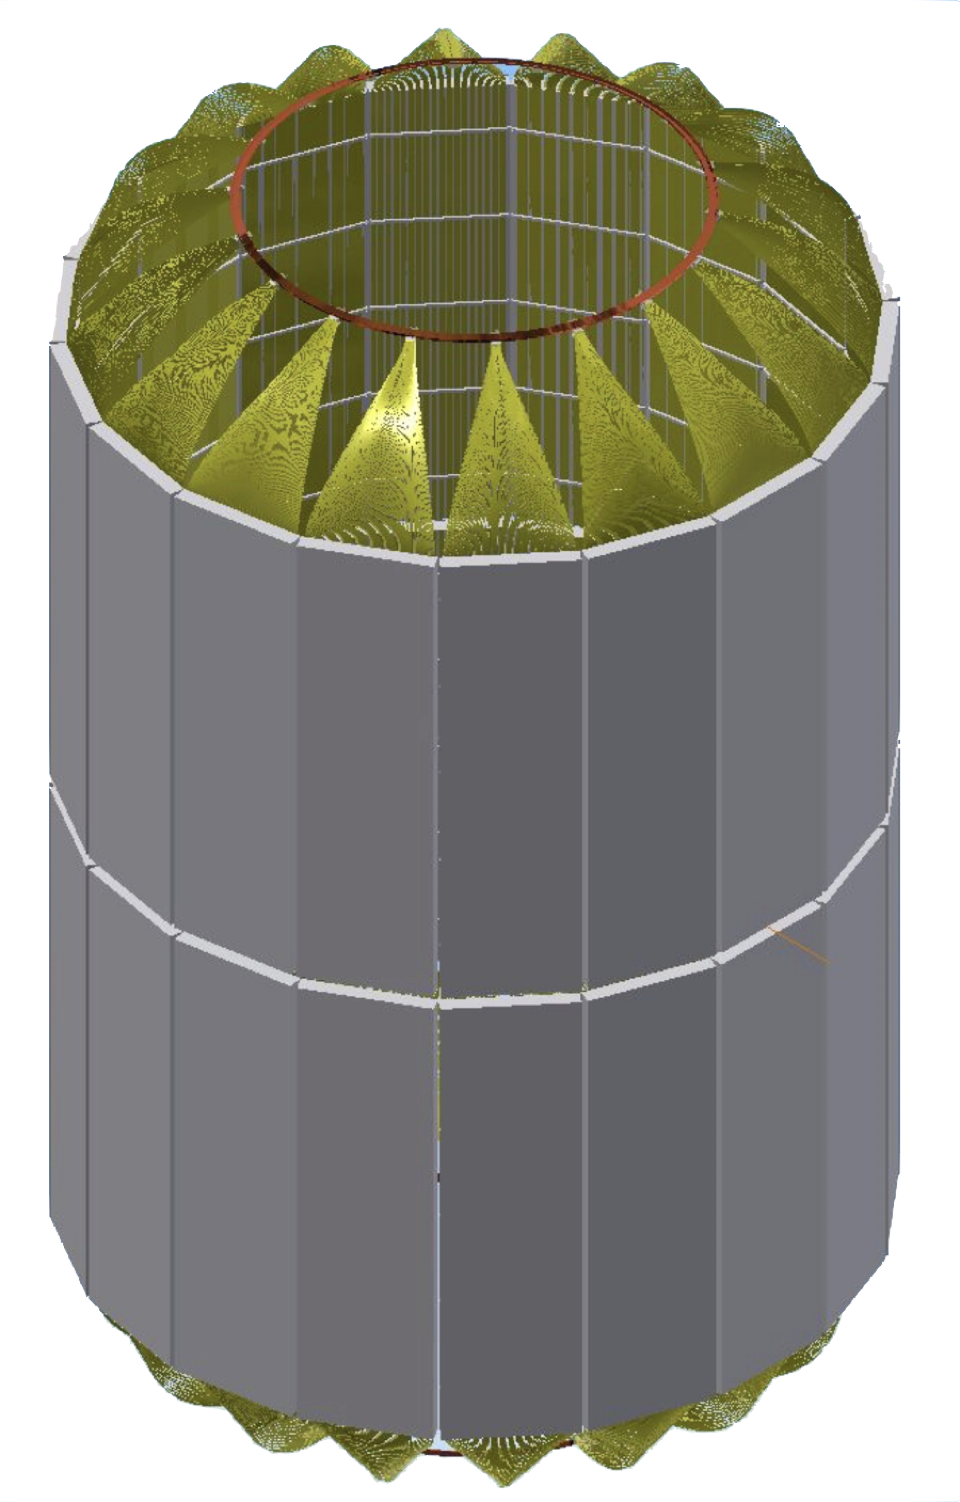
\includegraphics[scale=0.28]{cad.png}
%
%\column{0.50\textwidth}
%
%$\bullet~$ Measure the energy and \so\ with a Barrel Fibre Detector, read out by (cooled) SiPMs.
%
%$\bullet~$ Reduces background budget, simplifies mechanics and should allow improve energy resolution (smoother energy map). Improve energy resolution reduces all backgrounds. With 0.5\% FWHM, most backgrounds are reduced by a factor 2 and \BI\ by a factor 4. 
%
%\end{columns}
%\end{frame}


\begin{frame}{NEXT-HD sensitivity}

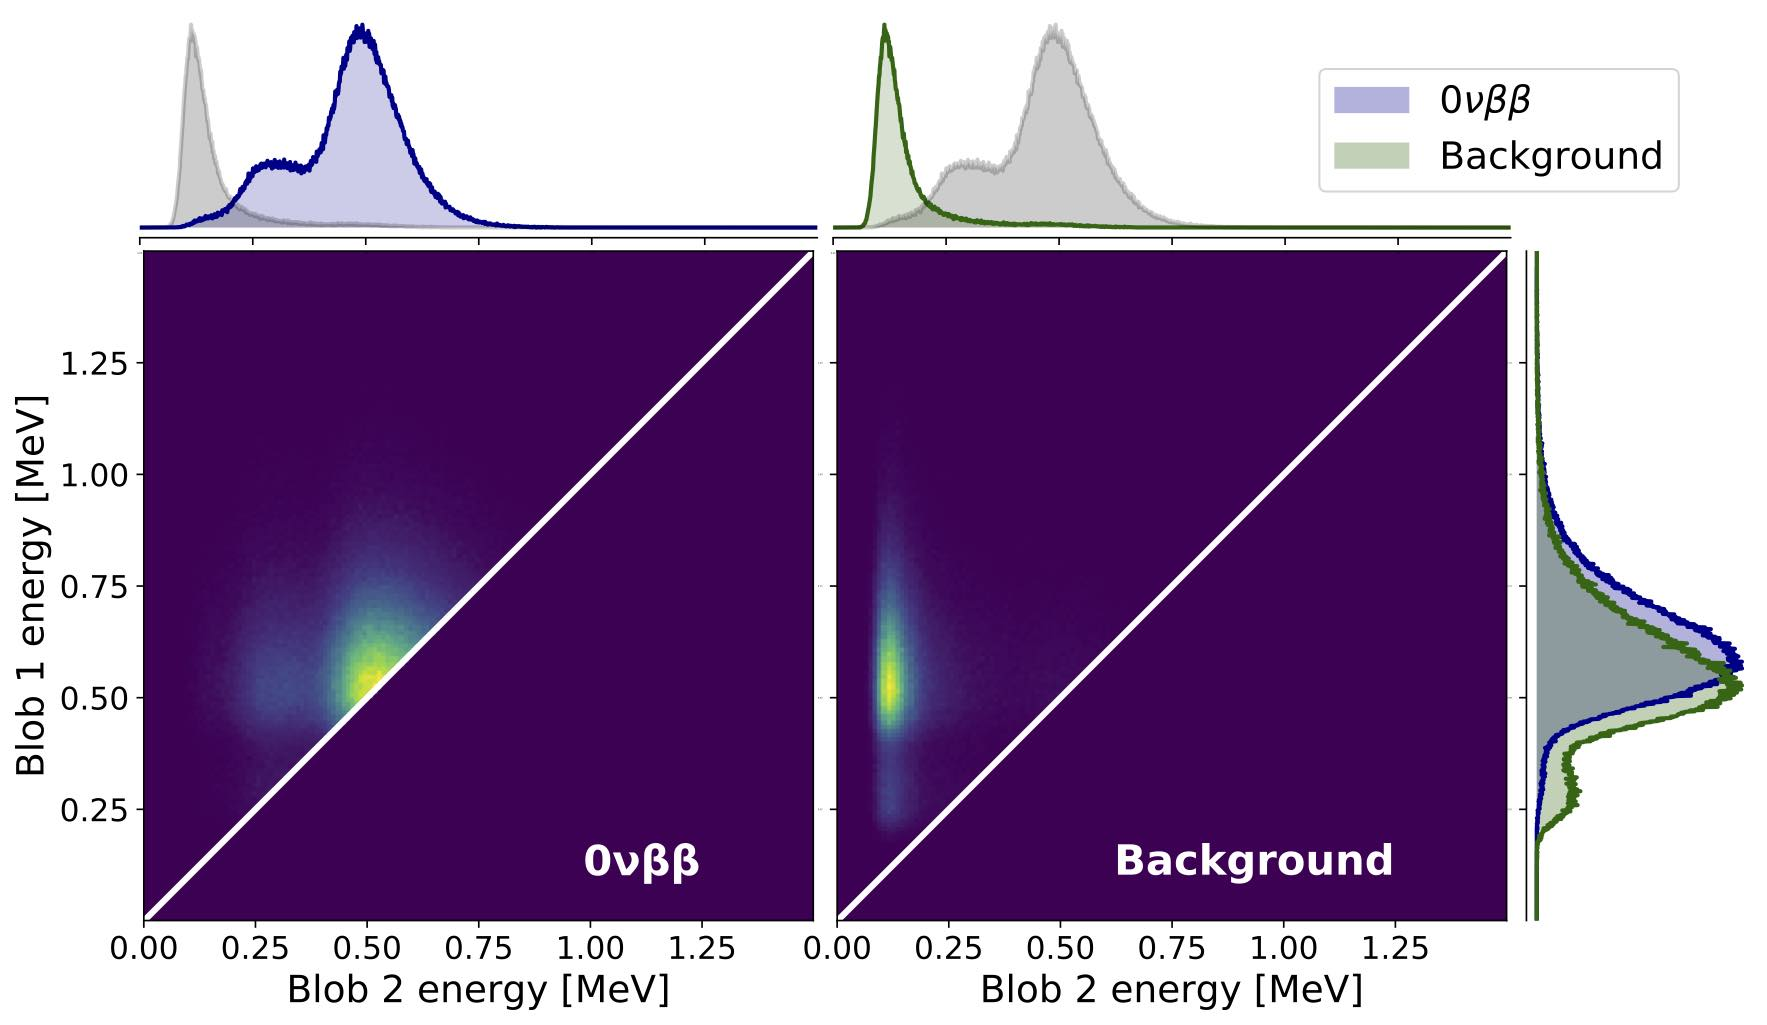
\includegraphics[width=0.55\textwidth]{BlobComparison.jpg}
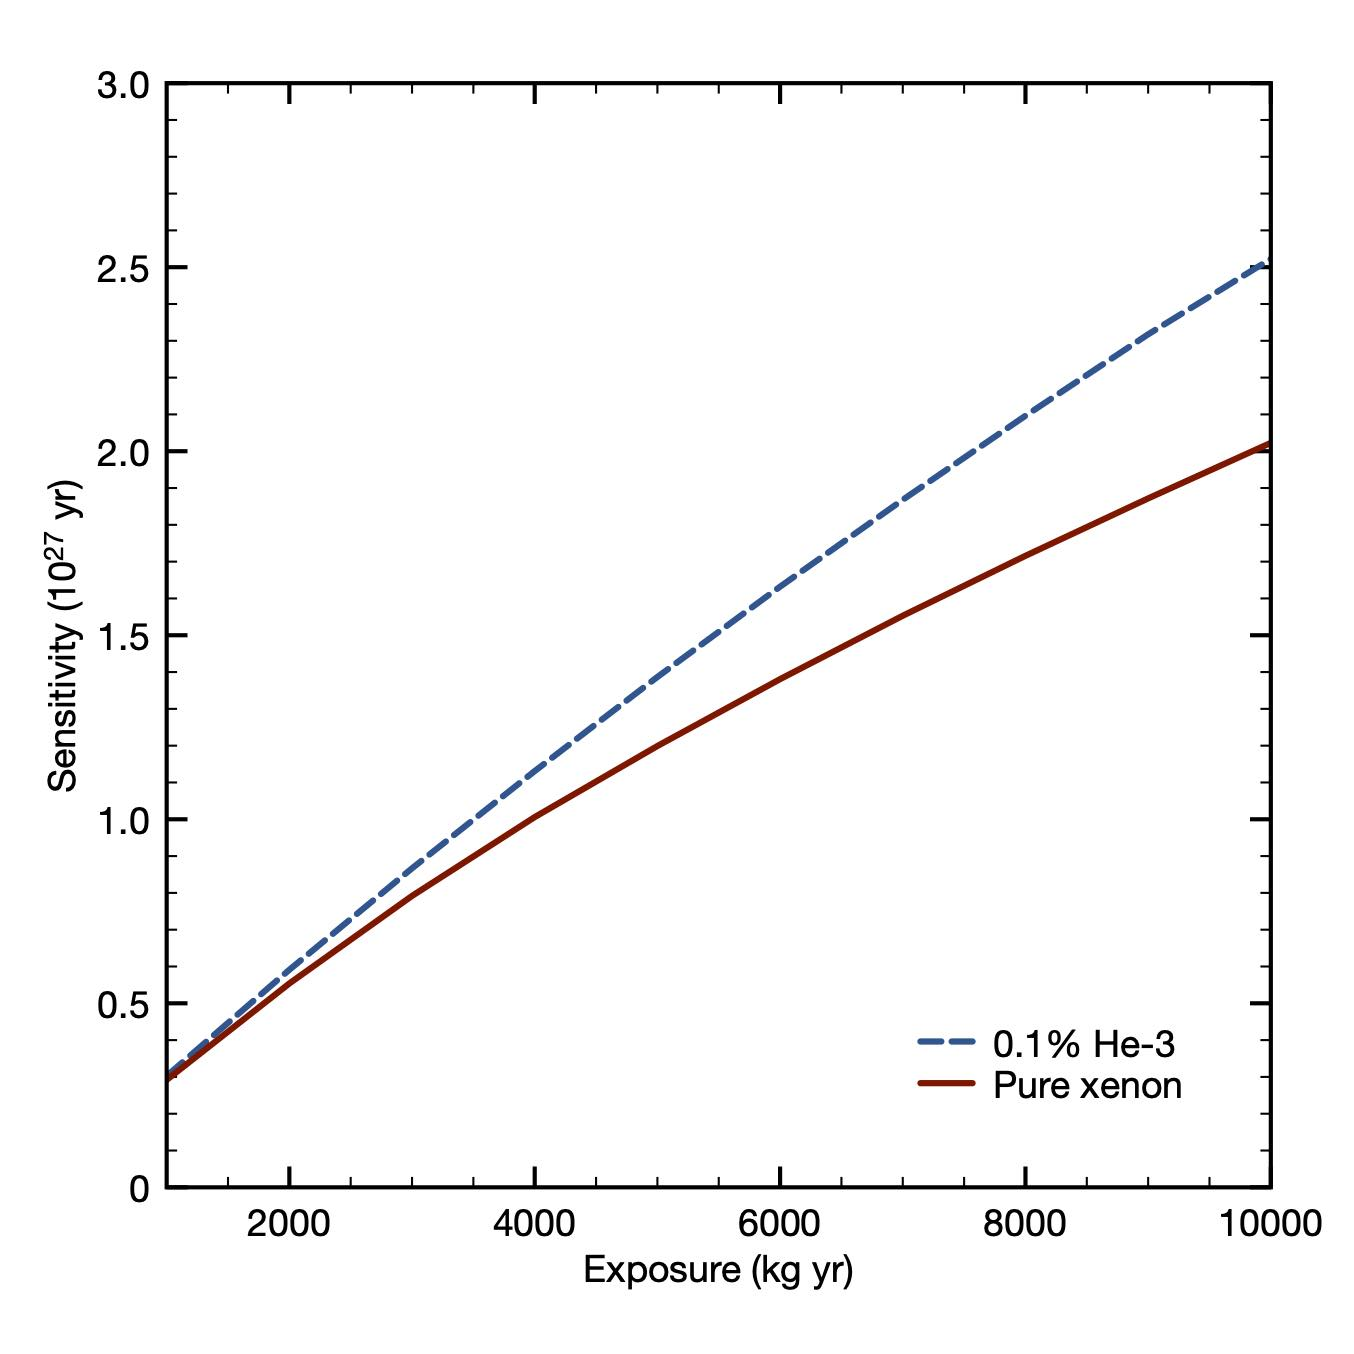
\includegraphics[width=0.40\textwidth]{sensitivity_nexthd_lsc.jpg}
\end{frame}

\begin{frame}{Barium Tagging}

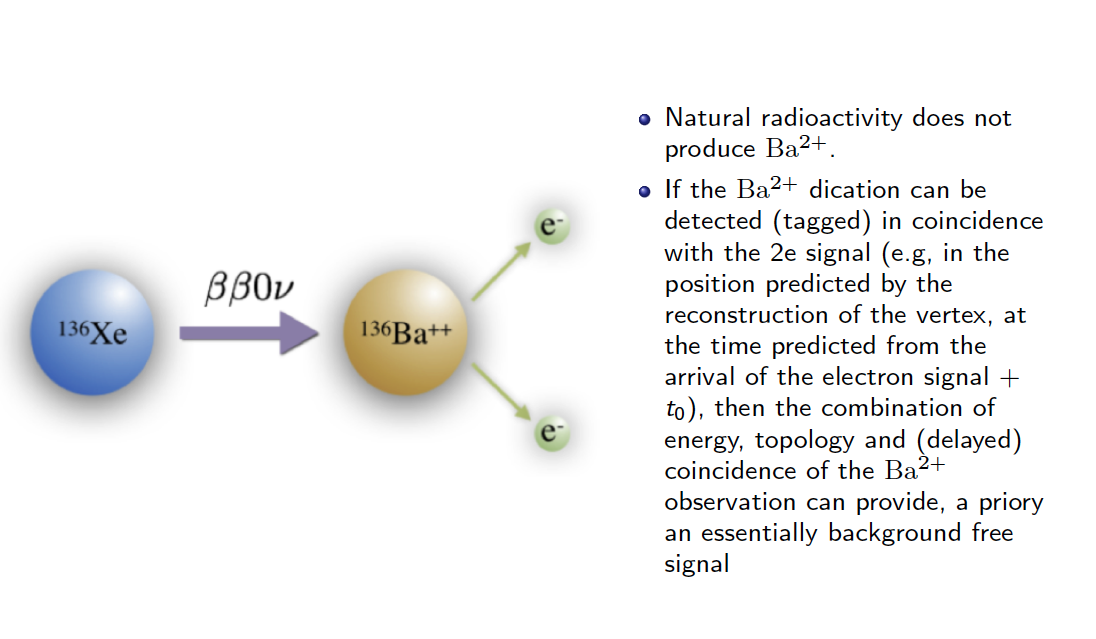
\includegraphics[width=0.90\textwidth]{Ba2pCartoon.png}

\end{frame}

\begin{frame}{Molecular sensors}
\begin{columns}
\column{0.50\textwidth}

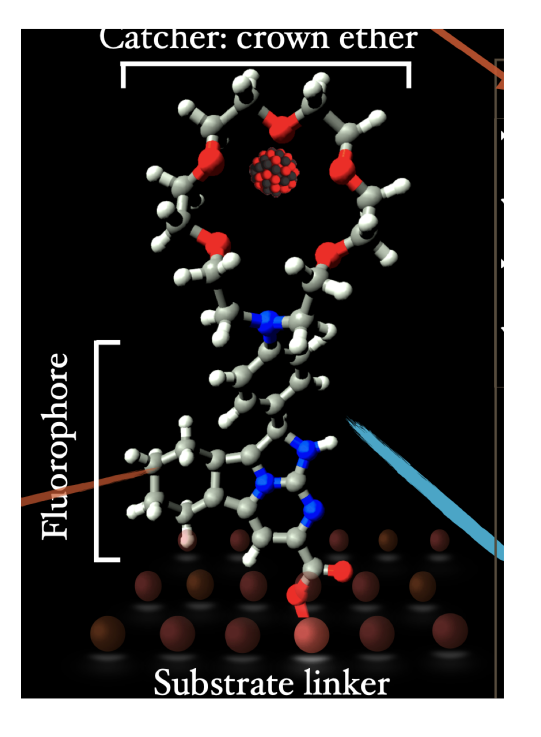
\includegraphics[width=0.70\textwidth]{molecularI.png}

\column{0.50\textwidth}
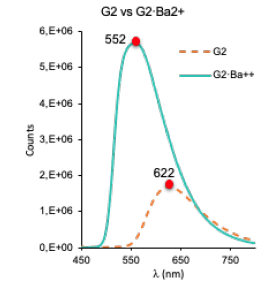
\includegraphics[width=0.80\textwidth]{g2.png}
\end{columns}
\end{frame}

\begin{frame}{NEXT-BOLD}
\begin{columns}
\column{0.50\textwidth}

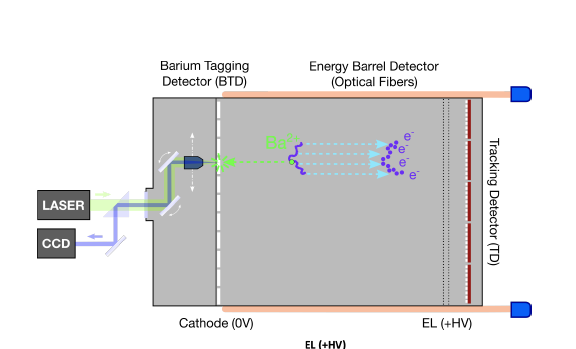
\includegraphics[width=0.99\textwidth]{nextBold.png}

\column{0.50\textwidth}
\includegraphics[width=0.99\textwidth]{boldPrototypes.png}
\end{columns}
\end{frame}

\begin{frame}{NEXT-BOLD}
\includegraphics[width=0.85\textwidth]{ba2Cern.png}
\end{frame}


\begin{frame}{NEXT at CERN: DRD1}


\begin{itemize}
\item The NEXT Collaboration, through one of our partner institutions, Universitat Politecnica de Valencia, co-developed the Scalable Readout System (SRS) for the RD51 Collaboration together with CERN and IFIN-HH Bucharest, under the leading of Hans Muller. This development resulted in agreement for exploitation of jointly owned intellectual property
(KN2288/KT/PH/203A) and the licence agreement for production and sale (agreement KR2680/KT/PH/203L). SRS has sold over 1 MCHF through the CERN stores, turning into a technical and scientific success.
\item SRS is being used as readout and DAQ for NEXT-100.
\item  In 2021, a successor for SRS, named SRSe, was proposed in the Snowmass MPGD white paper ”Trigger extensions for the Scalable Readout System SRS-e”. 
\item NEXT-UPV is heavily involved in the development of the high-level concentrator module (eFEC), one of the major elements of SRS-e
\end{itemize}

\end{frame}

\begin{frame}{NEXT at CERN: DRD2}

\begin{itemize}

\item NEXT is heavily involved in DRD2. Two NEXT members have leadership roles in DRD2, which covers the detector development for (liquid) noble element detectors. Roxanne Guenette (NEXT IB Chair) is spokesperson of the collaboration and is steering the scientific strategy of the detector R\&D. Justo Martin-Albo is Leader of the Work Package 2.2: Higher efficiency wavelength shifter and light collection, which attempt to increase the amount if VUV light collected by light detection systems. 
\item Among the DRD2 activities that NEXT members are involved in, there is Granular Light readout (for VUV), which relates to the development of dense silicon planes for energy and tracking in NEXT-HD.
\item  Furthermore, DRD2 is leading Work Package for Radiopurity \&
background mitigation, which includes the cooperation of national laboratories to develop new radio assay techniques and new materials with low-radioactivity for detector construction. 
\item All of these activities directly address some of the NEXT challenges and there is clear synergy between the NEXT activities and the DRD2 ones, where all being at CERN would allow for higher impact.
\end{itemize}
\end{frame}

\begin{frame}{NEXT at CERN: Software}

\begin{itemize}
\item We are collaborating with the CERN-Julia group (https://hepsoftwarefoundation.org/activities/juliahep.html) in the development of software and analysis tools using the Julian language. 
\item We are also active Geant4 developers 
\item We use the CERN cluster 
We have been using CERN computing services for many years. We use CERN computers heavily in our Monte Carlo productions. We would like to continue using those services (at the same level than now). 
\end{itemize}

\end{frame}
\begin{frame}{NEXT at CERN: R\&D in new instrumentation}


\begin{columns}
\column{0.50\textwidth}

\includegraphics[width=0.95\textwidth]{fatGem.png}

\column{0.50\textwidth}

\begin{itemize}
\item NEXT-HD/BOLD will have a diameter of 2.5 m, to compare with 1 m for NEXT-100. 
\item It is very hard to develop EL structures based on wires or meshes for those diameters. 
\item We are exploring the development of modular EL structures based on acrylic, similar to the "Fat Gems" developed at USC and CERN (collaboration with R. de Oliveira).
\end{itemize}
\end{columns}
\end{frame}



\begin{frame}{NEXT as CERN recognised experiment}

\begin{itemize}
\item We collaborate with CERN in a wide range of topics, ranging from software development to R\&D.  
\item We think that CERN beams (Isolde) could be a great asset for the NEXT-BOLD project (although we are late with respect to our original schedule we hope to move forward this project in the next two years). 
\item Ton-scale R\&D benefits at various levels from the expertise at CERN.
\item At the same time we are very active in various R\&D and bring our expertise to several CERN-based projects.
\item Our requests are small. We need modest computing support for Monte Carlo production and even more modest (temporary) office space. We benefit from human capital at CERN (experts at Isolde, R. Oliveira expertise, software groups) etc. We contribute with our own expertise to the projects in the lab.
\end{itemize}


\end{frame}


%\begin{frame}{Use Xe/He mixtures}
%\begin{columns}
%\column{0.50\textwidth}
%\includegraphics[scale=0.15]{xeHe.png}
%
%\column{0.50\textwidth}
%
%$\bullet~$ Reduces transverse diffusion by a factor 5 (thus the name, ``High Definition" NEXT).
%
%$\bullet~$ Combined with topology reconstruction with DNNs, should allow improving background rejection by a factor 2-3. 
%
%$\bullet~$ Addition of ${}^{3}He$ (high rate of capture of neutrons, 0.1 \% is enough) or deeper location to reduce the impact of \XES. 
%
%$\bullet~$ Deeper location also suppresses $\mu$ induced background. 
%
%\end{columns}
%\end{frame}
%
%\begin{frame}{Backgrounds in NEXT-HD}
%\begin{columns}
%\column{0.60\textwidth}
%\includegraphics[scale=0.40]{bkgndHD.png}
%\includegraphics[scale=0.40]{RadioHD.png}
%
%
%\column{0.40\textwidth}
%
%$\bullet~$ \TL\ and \BI\ contribute in the same amount. Dominant contribution is the ICS. R\&D to produce large amounts of ultra-pure radioactive copper is a must. 
%
%$\bullet~$ Deeper location to reduce non-radioactive backgrounds. \XES\ becomes subdominant if operating at LNGS (negligible at SNOLAB) 
%
%$\bullet~$ According to simulations a background rate below 1 cts/yer in the ROI can be achieved. 
%
%\end{columns}
%\end{frame}



\end{document}